%--------------------------------------------------------------------------------------------------
% ips-phd-thesis-eng-ieee.tex v1.2 (see the end of the file for modification history)
% Version 1.2 released 2015/04/13
%
% A template for creating a PhD thesis in English using the APA 6th edition reference formatting
% with several accompanying files.
% By Tea Tušar <tea.tusar@ijs.si>
%
% IMPORTANT NOTE: Biber must be used as the backhand for processing bibliographies, not bibtex!
%
% To compile this template, you need to run the following sequence of commands:
% 1. pdflatex  ips-phd-thesis-eng-ieee
% 2. biber     ips-phd-thesis-eng-ieee
% 3. makeindex ips-phd-thesis-eng-ieee (optional, if you want an index)
% 4. pdflatex  ips-phd-thesis-eng-ieee
% 5. pdflatex  ips-phd-thesis-eng-ieee
%--------------------------------------------------------------------------------------------------
\documentclass[phd,eng,ieee]{ipsthesis}
%
%--------------------------------------------------------------------------------------------------
%
% PREAMBULE
%--------------------------------------------------------------------------------------------------
%
% Files with bibliographies
\addbibresource{references_books.bib}
\addbibresource{references_cca.bib}
\addbibresource{references_crosslingual.bib}
\addbibresource{references_datasets_resources.bib}
\addbibresource{references_ER.bib}
\addbibresource{references_lsi.bib}
\addbibresource{references_mcca.bib}
\addbibresource{references_mine.bib}
\addbibresource{references_multiview_related.bib}
\addbibresource{references_optimization.bib}
\addbibresource{references_projects.bib}
\addbibresource{references_stats.bib}
\addbibresource{references_textmining.bib}
%
% Define here all other packages and commands you need for your thesis, for example:
\usepackage{color}
\usepackage{longtable}
\usepackage{algorithmic}
\usepackage{subcaption}
\usepackage{graphicx}
\usepackage{amsmath}

\newcommand{\RR}{\mathbb{R}}
\newcommand{\X}{\mathbb{X}}
\newcommand{\Y}{\mathbb{Y}}
\newcommand{\NN}{\mathbb{N}}
\newcommand{\sym}{\mathbb{S}}
\newcommand{\dataset}{{\cal D}}
\newcommand{\fracpartial}[2]{\frac{\partial #1}{\partial  #2}}
\newcommand\Prefix[3]{\vphantom{#3}#1#2#3}


%\usepackage{theorem}
\newtheorem{lemma}[theorem]{Lemma}
\newtheorem{proposition}[theorem]{Proposition}
\newtheorem{corollary}[theorem]{Corollary}
\newtheorem{assumption}[theorem]{Assumption}
\newtheorem{conjecture}[theorem]{Conjecture}

\newenvironment{notation}[1][Notation]{\begin{trivlist}
\item[\hskip \labelsep {\bfseries #1}]}{\end{trivlist}}

\newcommand{\abs}[1]{\lvert#1\rvert}
\newcommand{\norm}[1]{\lVert#1\rVert}



%--------------------------------------------------------------------------------------------------
%
% DOCUMENT
%--------------------------------------------------------------------------------------------------
\begin{document}
%--------------------------------------------------------------------------------------------------
%
% The cover page and spine are created separately using two .doc files provided by IPS.
%--------------------------------------------------------------------------------------------------
%
% FRONT MATTER
%--------------------------------------------------------------------------------------------------
%
\frontmatter
%
\selectlanguage{american}
\pagestyle{fancy}
%
% Title pages
%--------------------------------------------------------------------------------------------------
%
% INPUT FOR THE TITLE PAGES
%--------------------------------------------------------------------------------------------------
%
% Author
\author{Jan Rupnik}
%
% Title in English (use \protect\\ instead of \\ to create a line break)
\titleEnglish{Multi-View Canonical Correlation Analysis}
%
% Title in Slovene (use \protect\\ instead of \\ to create a line break)
\titleSlovene{Kanonična Korelacijska Analiza  za Več Množic Spremenljivk}
%
% Supervisor (title and name, affiliation)
\supervisorOne{Prof.\ Dunja Mladenić}{Artificial Intelligence Laboratory, Jožef Stefan Institute, Ljubljana, Slovenia}
%
% Co-supervisor (title and name, affiliation), optional
\supervisorTwo{Prof.\ John Shawe-Taylor}{Department of Computer Science, University College London, Gower Street, London WC1E 6BT, United Kingdom}
%
% Co-supervisor (title and name, affiliation), optional
%\supervisorThree{Prof.\ Name Surname3}{Institution3, Place, Country}
%
% Evaluation board chairman (title and name, affiliation)
\evaluationBoardChairman{Prof.\ Name SurnameA}{InstitutionA, Place, Country}
%
% Evaluation board member #1 (title and name, affiliation)
\evaluationBoardMemberOne{Prof.\ Name SurnameB}{InstitutionB, Place, Country}
%
% Evaluation board member #2 (title and name, affiliation)
\evaluationBoardMemberTwo{Prof.\ Name SurnameC}{InstitutionC, Place, Country}
%
% Date
\month{December}
\year{2015}
%
\maketitle 
%
% Dedication (optional)
%--------------------------------------------------------------------------------------------------
%
% INPUT FOR THE DEDICATION
%--------------------------------------------------------------------------------------------------
\dedication{To ...}
\makededication 
%
% Acknowledgments
%--------------------------------------------------------------------------------------------------
%
\chapter*{Acknowledgments}
\pdfbookmark[0]{Acknowledgments}{Acknowledgments}
%--------------------------------------------------------------------------------------------------

I would like to express great appreciation to my PhD supervisor Prof. Dunja
Mladenić and co-supervisor Prof. John Shawe-Taylor for their guidance and advice
throughout my studies. Special thanks go to Primož Škraba for his invaluable advice and contributions to my work.
I would also like to thank Marko Grobelnik for providing inspiration and encouragement for my research work.

Assistance provided by my collaborators Andrej Muhič, Blaž Fortuna, Gregor Leban
and Sabrina Guettes was greatly appreciated. It was my great pleasure working with you.
I would also like to thank my friends from UCL: Tom Diethe, David Roi Hardoon and Zakria Hussain
for great company and discussions during my visits to UCL.

My gratitude goes to the members of my doctoral committee, Prof. Nada Lavrač, Prof.
Bor Plestenjak and Prof. Nicolò Cesa-Bianchi, for their valuable comments and
remarks.

Finally, I wish to thank Zala, my parents Darja and Erik and my sister Nika
for their support and encouragement.

\rule{0.5\textwidth}{.4pt}

The author gratefully acknowledges funding by the projects
SMART (IST-5-033917-STP), X-LIKE (ICT-257790-STREP), MultilingualWeb (PSP-2009.5.2 Agr.\# 250500),
TransLectures (FP7-ICT-2011-7), PlanetData (ICT-257641-NoE), RENDER (ICT-257790-STREP), XLime (FP7-ICT-611346),
and META-NET (ICT-249119-NoE). 
%
% English abstract
%--------------------------------------------------------------------------------------------------
% 
\chapter*{Abstract}
\pdfbookmark[0]{Abstract}{Abstract}
%--------------------------------------------------------------------------------------------------

The English abstract should not take up more than one page.
%
% Slovene abstract, switch to slovene
\selectlanguage{slovene}
%--------------------------------------------------------------------------------------------------
%
\chapter*{Povzetek}
\pdfbookmark[0]{Povzetek}{Povzetek}
%--------------------------------------------------------------------------------------------------

Metode, ki temeljijo na matrični faktorizaciji, predstavljajo pomemben pristop k analizi vzorcev
in podatkovnemu rudarjenju. Naloge, ki jih lahko prevedemo na matrične razcepe, vključujejo izbiranje 
s sodelovanjem (ang. {collaborative filtering}), vstavljanje manjkajočih podatkov (ang. \emph{missing data imputation}), 
zmanjševanje dimenzij (ang. \emph{dimensionality reduction}, odstranjevanje šuma (ang. \emph{denoising}, vizualizacija
podatkov (ang. \emph{data visualization}) in eksploratorna analiza podatkov (ang. \emph{exploratory data analysis}).

V pričujoči disertaciji se ukvarjamo z \emph{večpogledno učenjem} (ang. \emph{multiview learning}), kjer
predpostavljamo, da imamo na podatke dva ali več \emph{pogledov} (ang. \emph{views}), kar konkretneje
pomeni, da imamo za vsako podatkovno instanco na voljo dve ali več množic značilk (ang. \emph{feature sets}),
ki predstavljajo različne poglede na nek objekt. Primer podatkovne množice primerne za večpogledno učenje
je množice parov slik in tekstovnih opisov, ki ustrezajo slikam. Predpostavljamo, da lahko slike in besedila
predstavimo kot objekte v dveh vektorskih prostorih, katerih dimenzije ustrezajo značilkam za analizo
slik oziroma besedil. V tem primeru iščemo vzorce (predstavljene kot funkcionale) v prostoru slik
in tekstovnem prostoru, ki so paroma močno povezani (na primer visoko korelirani vzdolž učne množice).

Kanonična Korelacijks Analiza (KKA) predstavlja enega izmed najpomembnejših pristopov za analizo
podatkov, kjer sta na voljo dva pogleda oziroma dve množici spremenjlivk. V pričujočem delu
preučujemo dve posplošitvi metode KKA za analizo poljubnega števila množic značilk: metoda
Vsote Korelacij (VKOR) (ang. \emph{Sum Of Correlations}) metode Vsote Kvadratov Korelacij (VKKOR).
Optimizacijski problem povezan s posplošitvijo VKOR se pojavi tudi v drugih problemih, med drugim
v teoriji regulacije, nalogah slepega ločevanja signalov (ang. \emph{Blind Source Signal Separation})
in analizi meritev funkcionalne magnetne resonance na skupinah subjektov.

Omenjeni posplošitvi VKOR in VKKOR preučimo z večih vidikov. Prvi prispevek k znanosti predstavlja
dokazano konvergentni algoritem za iskanje večih množic nelinearnih vzorcev, 
ki temelji na iterativni metodi za reševanje multivariatnih problemov lastnih vrednosti (ang. 
\emph{multivariate eigenvalue problems}). Dokažemo, da je problem KKRO v splošnem NP-težek,
kar nas privede do analize konveksne relaksacije in prevedbe na optimizacijsko nalogo
semidefinitnega programiranja (SDP) (ang. \emph{Semidefinite Programming}). Na podlagi
SDP formulacije predstavimo številne nove spodnje meje za vrednost globalno optimalne
rešitve. Čeprav so meje izračunjlive v polinomskem času, je njihov izračun v praksi
lahko težaven. Zato predstavimo pristop, ki temelji na zmanjšanju števila spremenljivk s
pomočjo naključnih projekcij. Predstavimo tudi aplikacijo posplošitev KKA na problemu
učenja jezikovno neodvisne mere podobnosti, kjer naletimo na problem manjkajočih
učnih podatkov. Pokažemo, da določena struktura manjkajočih podatkov pripelje do
poenostavitve optimizacijskega problema KKRO, ki ga prevedemo računsko manj zahteven 
problem lastnih vrednosti. Pokažemo, kako lahko uporabimo jezikovno neodvisno mero podobnosti
za medjezično povezovanje gruč dokumentov. Pristop uporabimo v sistemu za globalno analizo
tokov novic v večih jezikih.



\selectlanguage{american}
%
% Contents
\maketoc
%
% List of figures (required if the thesis contains figures)
\makelof
%
% List of tables (required if the thesis contains tables)
\makelot
%
% List of algorithms (required if the thesis contains algorithms)
\makeloa
%
% Abbreviations (optional)
%--------------------------------------------------------------------------------------------------
%
\chapter{Abbreviations}
%--------------------------------------------------------------------------------------------------
%
% A command that adjusts the of vertical positioning in the abbreviations and symbols chapters
\chapteradjust
% Correct the width of columns (23pt and 377pt) to fit your needs (they should sum up to 400pt).
% Use \cr instead of \\ to break lines.
\begin{longtable}{@{}p{53pt}@{\hspace{2pt} \dots \hspace{5pt}}p{347pt}@{}}
CCA & Canonical Correlation Analysis \cr
MCCA & Multiview Canonical Correlation Analysis \cr
KCCA & Kernel Canonical Correlation Analysis \cr
SUMCOR & Sum of Correlations \cr
SSCOR & Sum of Squared Correlations \cr
LSI & Latent Semantic Indexing \cr
SVD & Singular Value Decomposition \cr
TSVD & Truncated Singular Value Decomposition \cr
PCA & Principal Component Analysis \cr
CG & Conjugate Gradient \cr
SDP & Semidefinite Programming \cr
fMRI & functional Magnetic Resonance Imaging \cr
i.i.d & independently and identically distributed \cr
QCQP & Quadratically Constrained Quadratic Program \cr
%MEP & Multivariate Eigenvalue Problem \cr
BQO & Binary Quadratic Optimization \cr
TF & Term Frequency \cr
IDF & Inverse Document Frequency \cr
TFIDF & Term Frequency Inverse Document Frequency \cr
GB & Gigabyte \cr
GCCA & Generalized Canonical Correlation Analysis \cr
dim & dimension \cr
CCAR & Canonical Correlation Analysis Regression \cr
CL-VSM & Cross-Lingual Vector Space Model \cr
JPLSA & Joint Probabilistic Latent Semantic Analysis \cr
CPLSA & Coupled Probabilistic Latent Semantic Analysis \cr
PLTM & Polylingual Topic Models \cr
CPLSA & Coupled Probabilistic LSA \cr
PCLLSA & Probabilistic Cross-Lingual LSA  \cr
CL-ESA & Cross-Lingual Explicit Semantic Analysis \cr
OPCA & Oriented Principal Component Analysis \cr
% language abbreviations

\end{longtable} 
%
% Symbols (optional)
%--------------------------------------------------------------------------------------------------
%
\chapter{Symbols}
%--------------------------------------------------------------------------------------------------
%
% A command that adjusts the vertical positioning in the abbreviations and symbols chapters
\chapteradjust
% Correct the width of columns (10pt and 390pt) to fit your needs (they should sum up to 400pt).
% Use \cr instead of \\ to break lines.
\begin{longtable}{@{}p{40pt}@{\hspace{2pt} \dots \hspace{5pt}}p{360pt}@{}}
$\RR$	& real numbers \cr
$\RR^{m \times n}$	& matrices with $m$ rows and $n$ columns \cr
$\NN$	& natural numbers \cr
$\sym_{+}^n$ & space of symmetric positive semidefinite $n$-by-$n$ matrices \cr
$\sym_{++}^n$ & space of symmetric positive definite $n$-by-$n$ matrices \cr
$\vec{1}_k$ & column vector with $k$ dimensions with all coefficients equal to $1$ \cr
$\rho$ & correlation coefficient \cr
$\mu_X$ & empirical mean of a column sample matrix $X$ \cr
$Cov(\cdot, \cdot)$ & covariance function that takes two aligned sample matrices as input \cr
$\kappa(\cdot, \cdot)$ & kernel function \cr
$\norm{\cdot}_F$ & Frobenius norm \cr
$\norm{\cdot}_1$ & operator norm corresponding to $\ell_1$ norm \cr
$\phi(\cdot)$ & feature map from a set to a Hilbert space \cr

\end{longtable} 
%
% Glossary (optional)
%--------------------------------------------------------------------------------------------------
%
\chapter{Glossary}
%--------------------------------------------------------------------------------------------------

\emph{Correlation coefficient} measures the degree of linear dependence between two univariate random variables.\\
\emph{Canonical Correlation Analysis} is a way of measuring the linear relationship between two multidimensional variables.\\
\emph{Principal Component Analysis} is a dimensionality reduction technique based on maximization of variance.\\
\emph{Singular Value Decomposition} is a factorization of a real of complex matrix.\\
\emph{Vector Space Model} is a representation of textual data in a vector space, based on counting the occurrences of words, which correspond
to vector space dimensions.\\
\emph{Latent Semantic Indexing} is a text analysis technique based on the singular value decomposition of the corpus matrix.\\
\emph{$k$-means Clustering} is grouping algorithm that groups objects into groups according to their similarity.\\
\emph{Symmetric positive semidefinite matrix} is symmetric matrix with nonnegative eigenvalues.\\
\emph{Semidefinite programming} is a subfield of convex optimization concerned with the optimization of a linear objective function over the intersection of the cone of positive semidefinite matrices with an affine space.\\
\emph{Dual Representation} expresses vectors as linear combinations over the training set.\\
\emph{Hilbert space} is a vector space equipped with an inner product.\\
\emph{Kernel functions} provide a way to manipulate data as though it were projected into a higher dimensional space.\\
\emph{Kernel methods} are a class of algorithms for pattern analysis, based on embeddings into a Hilbert space.\\

%--------------------------------------------------------------------------------------------------
%
% MAIN MATTER
%--------------------------------------------------------------------------------------------------
%
\mainmatter
%
% Introduction
%--------------------------------------------------------------------------------------------------
%
\chapter{Introduction}
%--------------------------------------------------------------------------------------------------

\emph{Pattern analysis} is the process of finding structure or regularity in a set of data. For example,
if each data instance represents a point in a vector space, we might be interested in the following question: does the dataset lie
in a lower dimensional subspace (does it admit a more compact representation)? In this case, the subspace represents a pattern (structure or regularity)
discovered in the data. Principal Component Analysis provides a solution to such a question.

This thesis deals with finding patterns in datasets that exhibit a \emph{multi-view} aspect: that is, for
each instance of data there are two or more representations (views) available. We refer to such datasets as
\emph{aligned} (multi-view) datasets. As an example of a two-view dataset, consider a dataset where each instance is represented by a visual image and
a textual description. Another example is a \emph{parallel multi-lingual corpus},
where given $n$ languages, each data instance consists of $n$ documents, one for each language and the documents are related by being
translations of each other. The patterns that we are interested in represent regularities within each view
that have associated regularities in other views. For example, when dealing with text, a type of pattern that is often of interest
is a distribution over words from a fixed vocabulary, referred to as a \emph{topic vector}. Given a collection of documents
in a single language, a typical problem is to find relevant topic vectors that summarize the document collection. The multi-view
variant of the problem then corresponds to finding sets of multiple representations of topic vectors (one per language).
Methods that extract such multi-representation patterns represent the main subject of the thesis.

There are several possible applications of such an analysis. The patterns themselves can be of interest
for explorative analysis. For example, given an aligned dataset of fMRI brain scans and visual images that were
shown to the subjects as scans were taken, we can investigate how the brain functions by looking at
relationships between brain activation regions and patterns in visual images.
Another example of application is to use the multi-view patterns as maps into a
representation independent space. For example, representing visual images and textual descriptions in the same
space can be used for cross-modal information retrieval, where one searches for images relevant to a query text,
(or documents relevant to a given image) by using standard information retrieval techniques. 
In addition, the optimization problem related to one of the generalizations of Canonical Correlation Analysis (CCA) that we
study appears in applications that range from control theory, blind source separation to multiple subject fMRI analysis.

\section{Overview and Questions Addressed}

We will now provide a high-level overview of the results presented in the thesis and highlight the related work
that motivated or enabled the results, all of which is summarized in Figure~\ref{fig:position_of_work}.
Canonical Correlation Analysis (CCA)~\cite{Hotelling}, a well established method that looks for patterns in two-view
datasets, has been extended by other authors in several ways: a nonlinear extension was proposed in~\cite{FBMJ}, which
was later applied to text in~\cite{vinokourov2002inferring}. It has been extended to more than two sets of variables
in~\cite{Horst}, where a formulation called \emph{Sum of Correlations} (SUMCOR) was presented, together with an iterative
algorithm to finding local solutions, known as the \emph{Horst's algorithm}. Results on global optimality of a subset
of SUMCOR problems was established in~\cite{GlobalMEP} and~\cite{GlobalMEP2}. Several alternative generalizations
of CCA were proposed in~\cite{Kettenring}, where the most relevant extension to the thesis is the
\emph{Sum of Squared Correlations} (SSCOR).

The thesis starts with two questions:
\begin{itemize}
\item How can we extend the Horst's algorithm to handle nonlinear patterns and how to find several sets of canonical vectors? Does the extension provably converge?
\item What is the computational complexity of the SUMCOR problem formulation?
\end{itemize}
We present an extension that is closely related to~\cite{FBMJ} and show that it does converge to local solutions. We prove that in
general the computational complexity of the SUMCOR problem is NP-hard.
 In light of these results, several questions arose:
\begin{itemize}
\item Can we find a convex relaxation of the problem?
\item Can we obtain computationally tractable bounds on the SUMCOR objective?
\end{itemize}
We show how to relax the problem to an instance of a Semidefinite Programming (SDP), whose solutions yield
computable bounds on global optimality. The results related to SUMCOR complexity and SDP relaxations
are available in~\cite{DBLP:journals/corr/abs-1302-0974} and submitted for publication.

Applying the theory to practice opened up the following questions:
\begin{enumerate}
\item How to apply the SDP bounds to high dimensional data?
\item How can one use the methods to perform cross-lingual document analysis?
\item How does one handle missing data?
\end{enumerate}
We addressed the questions in the following way:
\begin{enumerate}
\item We proposed a preprocessing step that reduces the number
of variables in the SDP derived from a SUMCOR problem instance which makes the relaxation computationally tractable. 

\item We present the methodology for building cross-lingual similarity functions and apply it
to the task of cross-lingual cluster linking. The application is relevant to global analysis of high-volume
multi-lingual news streams.

\item We address the problem of missing data in our application to cross-lingual text mining for datasets where
data was missing in a structured way and show that under certain assumptions, the SSCOR problem formulation
can be reduced to a low-dimensional eigenvalue problem. The results related to SSCOR reduction and
cross-lingual applications are available in~\cite{rupnikJAIR}.
An alternative application of the SSCOR reformulation to cluster linking is published in~\cite{Belyaeva201564}.
\end{enumerate}
\begin{figure}[t]
\centering
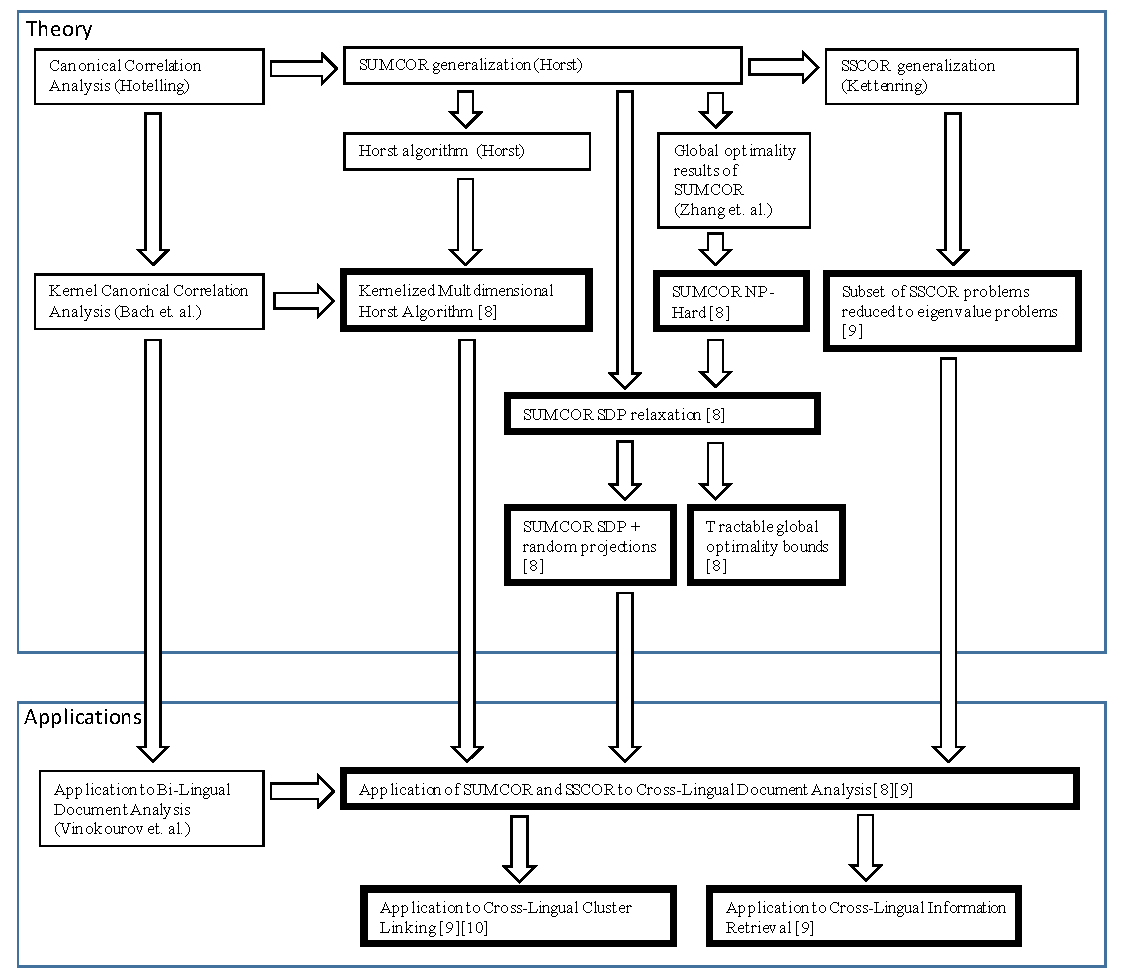
\includegraphics[width=1\textwidth]{figures/position_of_work.pdf}
\caption[The main contributions and related work]{The main contributions, represented by text boxes with thick border, are
positioned with respect to the related work.}
\label{fig:position_of_work}
\end{figure}

\section{Scientific Contributions}

We now list the main scientific contributions of the thesis and their references:
\begin{itemize}
\item A novel algorithm based on the Horst's algorithm that can extract several sets of nonlinear patterns ~\cite{DBLP:journals/corr/abs-1302-0974}
\item A proof that in general the Sum of Correlations problem is NP-hard ~\cite{DBLP:journals/corr/abs-1302-0974}
\item A semidefinite programming relaxation of the SUMCOR problem and
several new bounds on global optimization of the SUMCOR problems~\cite{DBLP:journals/corr/abs-1302-0974}
\item A novel approach to apply the SDP bounds on high-dimensional data~\cite{DBLP:journals/corr/abs-1302-0974}
\item A novel approach to building cross-lingual similarity functions and its application to cross-lingual information retrieval and cross-lingual cluster linking~\cite{rupnikJAIR}\cite{Belyaeva201564}
\item Addressing the missing data problem, a novel reduction of a subset of SSCOR problems to eigenvalue problems~\cite{rupnikJAIR}
\end{itemize}

\section{Thesis Structure}

The rest of the thesis is structured as follows. Chapter~\ref{chap:notation} introduces notation and some
definitions. For background we describe three pattern analysis methods that are the most relevant
for the thesis and explain how they can be adapted for analysis of nonlinear patterns in Chapter~\ref{chap:background}. Chapter~\ref{chap:extensions}
introduces a central problem of the thesis: generalizations of Canonical Correlation Analysis (CCA) and the original
contributions that extend the method to nonlinear and higher-dimensional setting. In Chapter~\ref{chap:relaxations}
we prove the result on the complexity of a particular generalization and study global optimality guarantees based
on semidefinite relaxations. Chapter~\ref{chap:crosslingual} discusses an application of multiview learning
to building cross-lingual similarity models. We show how a particular structure of the data can be exploited
to express a particular generalization of CCA as an eigenvector problem. Chapter~\ref{chap:applications} then
shows how the cross-lingual similarity measures can be used to perform cross-lingual cluster linking, relevant
for large scale monitoring of global news in multiple languages. In Chapter~\ref{chap:experiments} several experiments
are presented both on synthetic and real datasets. Finally, Chapter~\ref{chap:conclusions} concludes the thesis
and discusses possible future directions. 

%--------------------------------------------------------------------------------------------------
%
\chapter{Notation and definitions}\label{chap:notation}

We first introduce the notation we use throughout the thesis:
\begin{itemize}
\item Column vectors are denoted by lowercase letters, e.g. $x$ and matrices are denoted by uppercase letters, e.g. $X$.
\item Subscripts are used to enumerate vectors or matrices, e.g. $x_1, x_2$, $X_1$, except in the
special case of the identity matrix, $I_n$ and the zero matrix $0_{k,l}$. In these cases, the subscripts denote row and column dimensions.
\item We use superscripted symbol $T$ for vector and matrix transpose, e.g. $x^T$
\item Let $\norm{v}$ or $\norm{v}_2$ denote the $\ell_2$ norm of the vector $v$ and $\norm{A}_F$, $\norm{A}_1$ and $\norm{A}_2$ to denote the Frobenious norm and operator norms induced by $1$-norm and $2$-norm respectively.
\item MATLAB notation~\cite{golub}
\begin{itemize}
\item The $i$-th element of vector $x$ is denoted by $x(i)$ and the matrix entry in the $i$-th row and $j$-th column is denoted by $X(i,j)$.
\item The $i$-th row of matrix $X$ is denoted by $X(i,:)$ and the $j$-th column by $X(:,j)$.
 matrix elements, rows and columns {(e.g. ${X(i,j), X(i,:), X(:,j)}$)}
\item Matrix concatenation: $[A B]$ represents horizontal concatenation and $[A; B]$ represents vertical concatenation.
\item $diag(v)$ denotes a diagonal matrix whose diagonal entries correspond to vector $v$.
\item $\vec{1}_k$ denotes a column vector with $k$ elements all equal to $1$.
\end{itemize}
\item Spaces
\begin{itemize}
 \item $\RR^n$ denotes the $n$-dimensional real vector space
 \item $\RR^{n\times m}$ denotes the $(n \cdot m)$-dimensional vector space used when specifying
 matrix dimensions.
 \item $\NN$ denotes the natural numbers.
 \item $\sym_n^{+}$ denotes the space of symmetric positive definite $n$-by-$n$ matrices.
\end{itemize}
\item Random vectors are denoted by calligraphic letters, e.g. $\mathcal{X}$ and $\mathcal{X} \in \RR^n$ denotes their dimension.
\end{itemize}


\section{Sample data sets and the multiview assumption}
The following definitions will be relevant for our discussion of kernel versions of the methods relevant to this thesis.

\begin{definition}\label{def:notation:sample_dataset}
A \emph{sample dataset} with $\ell$ samples and $n$ dimensions is a set
$$ S := \lbrace x_1, \ldots, x_\ell \rbrace, $$
 where $x_i \in \RR^n$ are  generated independently and identically distributed (i.i.d.) according to
an underlying distribution. 
\end{definition}

\begin{definition}\label{def:notation:sample_matrix}
A \emph{$n\times\ell$ sample matrix} based on a dataset $S$ with $\ell$ samples and $n$ dimensions is obtained by horizontal concatenation:
$$ X := \left[ x_1 \cdots x_\ell \right]. $$ 
\end{definition}

\begin{definition}\label{def:notation:multiview_dataset}
A \emph{multiview sample dataset} with $\ell$ samples and $m$ views is a set:
$$ S = \big\{ \left( x_1^{(1)},\ldots, x_1^{(m)} \right), \ldots, \left( x_\ell^{(1)}, \ldots, x_\ell^{(m)} \right) \big\}, $$
 where $x_i^{(j)} \in \RR^{n_j}$ corresponds to the $j$-th view of the $i$-th sample. We assume that each sample point was generated independently and identically distributed (i.i.d.)
  according to an underlying distribution with a specific structure.
   We assume that the samples represent different views of an underlying object, that is, the observed random vectors
  are functions of an unobserved random vector:
$$ \left( \mathcal{X}^{(1)}, \ldots, \mathcal{X}^{(m)} \right) = \left( f_1(\mathcal{O}), \ldots, f_m(\mathcal{O}) \right).$$  
\end{definition}

\begin{definition}\label{def:notation:multiview_aligned_matrices}
A \emph{multiview aligned matrices} based on a dataset $S$ with $\ell$ samples and $m$ views is a set sample matrices, where the $i$-th view
matrix is obtained by horizontal concatenation:
$$ X_i := \left[ x_1^{(i)} \cdots x_\ell^{(i)} \right]. $$
In general, we will say that two matrices are aligned, if their columns form observation vector pairs, related to a multiview dataset.
\end{definition}

\begin{definition}\label{def:notation:multiview_stacked_matrix}
A \emph{multiview stacked matrix} based on a dataset $S$ with $\ell$ samples and $m$ views is a matrix obtained by 
vertically concatenating the multiview aligned matrices:
$$ X := \left[ X_1; \cdots X_m; \right].$$
\end{definition}

\begin{definition}\label{def:notation:centered_matrix}
The sample matrix is centered if its rows sum to zero.
\end{definition}

\begin{definition}\label{def:notation:empirical_mean}
Given a $n\times\ell$ sample matrix $X$, the \emph{empirical mean} $\mu_X \in \RR^n$ is computed as:
$$ \mu_X(i) = \frac{1}{\ell} \sum_j X(i,j).$$
\end{definition}

\begin{definition}\label{def:notation:empirical_covariance}
Given a sample matrix $X \in n \times \ell$
 the empirical covariance is defined as:
$$ Cov(X) := \frac{1}{n-1}(X - \mu_{X} \cdot \vec{1}_\ell^T)\cdot(X - \mu_{X} \cdot \vec{1}_\ell^T)^T.$$
\end{definition}

\begin{definition}\label{def:notation:empirical_variance}
\emph{Empirical variance} $Var(X)$ is defined as the empirical covariance for single dimensional sample matrices, that is, when $n$ equals $1$.
\end{definition}

\begin{definition}\label{def:notation:empirical_cross_covariance}
Given two aligned sample matrices $X_1 \in n_1 \times \ell$ and $X_2 \in n_2 \times \ell$ 
 the empirical cross-covariance is defined as:
$$ Cov(X_1, X_2) := \frac{1}{n-1}(X_1 - \mu_{X_1} \cdot \vec{1}_\ell^T)\cdot(X_2 - \mu_{X_2} \cdot \vec{1}_\ell^T)^T.$$
\end{definition}


\section{Kernel methods}
The following definitions will be relevant for our discussion of kernel versions of the methods relevant to this thesis. For definitions
of standard concepts from topology we refer the reader to standard texts~\cite{bourbaki1998general}.

\begin{definition}\label{def:notation:metric_space}
A \emph{metric space} is an ordered pair $(M,d)$, where $M$ is a set and $d: M \times M \rightarrow \RR$ is a \emph{metric} on $M$, i.e., 
a function which satisfies for all $x,y,z \in M$:
$$d(x,y) \geq 0$$ 
$$d(x,y) = 0 \Longleftrightarrow x = y$$
$$d(x,y) = d(y,x)$$
$$d(x,z) \leq d(x,y) + d(y,z)$$
\end{definition}

\begin{definition}\label{def:notation:cauchy_sequence}
Let $X$ be a metric space equipped with a metric $d: X \times X \rightarrow \RR$. A \emph{Cauchy sequence} is a sequence
of elements $x_1, x_2, x_3, \ldots$ if for every $\epsilon > 0$ there is a positive integer $N$ such
that for all $m,n > N$:
$$ d(x_m, x_n).$$
\end{definition}

\begin{definition}\label{def:notation:complete_space}
A metric space $X$ is complete, if every Cauchy sequence of elements in $X$ converges to an element of $X$.
\end{definition}

\begin{definition}\label{def:notation:separable_space}
A topological space $H$ is \emph{separable} if it contains a countable dense subset; that is, there
exists a sequence ${x_n}_{n=1}^{\infty}$ such that every nonempty open subset of the space contains at least
on element of the sequence.
\end{definition}

\begin{definition}\label{def:notation:hilbert_space}
A \emph{Hilbert Space} $H$ is an inner product space that both \emph{separable} and \emph{complete}. 
\end{definition}

\begin{definition}\label{def:notation:kernel_function}
Let $V \subset \RR^n$. A \emph{kernel} is a function $\kappa: V \times V \rightarrow \RR$ that satisfies:
$$ \kappa(x,y) = \lbrace \phi(x), \phi(y) \rbrace, $$
where $\phi: V \rightarrow H$ is a function from $V$ to a Hilbert space.
\end{definition}

\begin{definition}\label{def:notation:kernel_matrix}
Given a sample matrix $n\times\ell$ $X$ and a kernel function $\kappa$, we define a \emph{kernel matrix} $K \in \RR^{\ell \times \ell}$ as:
$$ K(i,j) := \kappa(x_i, x_j).$$ 
\end{definition}
%--------------------------------------------------------------------------------------------------
%
\chapter{Background}\label{chap:background}
%--------------------------------------------------------------------------------------------------

The central subjects in the thesis revolve around statistical approaches to finding structure in one, two or more sets of variates. We will
introduce two methods that find structure in a single set of variates: $k$-means clustering and Singular Value Decomposition (SVD) for dimensionality reduction, which is closely related to Principal Component Analysis (PCA). We will then present Canonical Correlation Analysis (CCA), a method for studying two sets of variates. We will also briefly cover kernel method extensions of the methods.


\section{$k$-means Decomposition}\label{chap:background:kmeans}

The $k$-means algorithm~\cite{kmeans} is perhaps the most well-known and widely-used clustering algorithm. In spirit of analysis on multiview methods that is to be presented, we will formulate $k$-means as a matrix factorization problem. Given a $n \times \ell$ sample matrix (Definition~\ref{def:notation:sample_matrix})
the goal is to find a best rank $k$ approximation under additional constraints:

\begin{equation}\label{eq:background:kmeans:opt}
\begin{aligned}
& \underset{C \in \RR^{n \times k}, P \in \RR^{\ell \times k}}{\text{minimize}}
& & \norm{X - C \cdot P^T}_F^2, \\
& \text{subject to}
& & P(i,j) \in \{0,1\}, \quad \forall i,j \\
& & & \sum_j P(i, j) = 1, \quad \forall i.
\end{aligned}
\end{equation}

The interpretation of the additional constraints on matrix $P$ is that they force each sample vector
(column in $X$) to select precisely one column of $C$ to approximate it and the objective function
corresponds to minimizing a sum of squared errors made by approximating points with centroids.

The matrix $C$ in Equation~\ref{eq:background:kmeans:opt} is uniquely defined given $P$, since for any given set
of points in $\RR^n$, the point that minimizes the sum of squared distances to the set is the mean. Since each
column of $P$ selects a subset of columns of $X$, $C$ can be expressed as:
\begin{equation}\label{eq:background:kmeans:centroids}
\begin{aligned}
 C := X\cdot P diag(\vec{1}_\ell^T \cdot P)^{-1} P^T,
\end{aligned}
\end{equation}
where the inverse of the diagonal matrix corresponds dividing by the set size when computing the mean ($\vec{1}_\ell^T \cdot P$ counts
the number of points assigned to each of the $k$ clusters). In addition, given $C$, the assignment $P$ that
minimizes the sum of squared errors can be found by:
\begin{equation}\label{eq:background:kmeans:assignments}
\begin{aligned}
P(i, j^*) = 1,\quad \textnormal{where}\quad j^* = argmin_j \norm{X(:,i) - C(:,j)}
\end{aligned}
\end{equation}

A popular approach~\cite{kmeans} to solving the problem in Equation~\ref{eq:background:kmeans:opt} is to start with an initial assignment and alternate between updating $C$ given $P$ and vice
versa. The approach is widely used in practice, even though it is susceptible to finding local minima. In general, the problem is known to be NP-hard~\cite{aloise2009np}.

\section{Singular Value Decomposition}\label{chap:background:svd}

The second factorization based approach that is relevant to our work is based on the Truncated Singular Value Decomposition~\cite{golub} (TSVD). It is closely
related Principal Component Analysis~\cite{Pearson1901On} (PCA), a well established approach to dimensionality reduction.

Given a $n \times \ell$ sample matrix (Definition ~\ref{def:notation:sample_matrix})
the goal is to find a best rank $k$ approximation under additional constraints:

\begin{equation}\label{eq:background:svd:opt}
\begin{aligned}
& \underset{U \in \RR^{n \times k}, S \in \RR^{k \times k}, V \in \RR^{\ell \times k}}{\text{minimize}}
& & \norm{X - U \cdot S \cdot V^T}_F, \\
& \text{subject to}
& & U^TU = I_k \\
& & & V^TV = I_k \\
& & & S = diag(\sigma), \quad \sigma \in \RR^k, \quad \sigma(i) \geq 0.
\end{aligned}
\end{equation}

The method of PCA is based on a low rank decomposition of the empirical covariance matrix, computed based on the sample matrix. The main
idea is to find a subspace that accounts for as much as variability in the data as possible. The first principal component is defined
as the one-dimensional subspace that maximizes the variance of the data when projected onto it. Formally, it solves the following problem:
\begin{equation}\label{eq:background:pca:single}
\begin{aligned}
& \underset{u \in \RR^{n}}{\text{maximize}}
& & Var(u^T \cdot X), \\
& \text{subject to}
& & \norm{u} = 1.
\end{aligned}
\end{equation}


The other principal vectors can be obtained by deflation~\cite{shawe-taylor04kernel}, or equivalently solving the eigenvalue problem:
\begin{equation}\label{eq:background:pca:opt}
\begin{aligned}
& \underset{U \in \RR^{n \times k}}{\text{minimize}}
& & \norm{Cov(X) - U \cdot \Lambda \cdot U^T}_F, \\
& \text{subject to}
& & U^TU = I_k \\
& & & \Lambda = diag(\lambda), \quad \lambda \in \RR^k.
\end{aligned}
\end{equation}

One of the main applications of PCA is as a dimensionality reduction technique, where the data is projected to the space
spanned by the normalized eigenvectors (also called principal vectors). In typical applications a truncated eigenvalue decomposition where
principal vectors with small eigenvalues are discarded (similar to truncated SVDs).

If the data matrix is centered, then the solution $U$ of TSVD and the eigenvector basis $U$ of PCA will coincide.


\section{Canonical Correlation Analysis}\label{chap:background:cca}

Canonical Correlation Analysis (CCA) ~\cite{Hotelling} is a general procedure for studying
relationships between two sets of random variables. It is based on analyzing the
cross-covariance matrix between two random vectors with the aim of identifying
linear relationships between them. We will start with intuitions and then give a formal presentation.

Roughly speaking, given two random vectors $\mathcal{X}^{(1)}$ and $\mathcal{X}^{(2)}$
we are interested in ``non-trivial'' pairs of functions $(f^{(1)},f^{(2)})$ such that
there is a ``dependence'' between $f^{(1)}(\mathcal{X}^{(1)})$ and $f^{(2)}(\mathcal{X}^{(2)})$.
The ``dependence'' we consider is linear (possibly in a Hilbert space). The ``non-triviality''
of the functions is a requirement that guards us against trivial solutions, such
as $f^{(1)}(x) := 0 \cdot x$, $f^{(2)}(y) := 0 \cdot y$ - that is,
$f^{(1)}(\mathcal{X}^{(1)})$ and $\mathcal{X}^{(1)}$ should share some information,
and analogously for $f^{(2)}(\mathcal{X}^{(2)})$ and $\mathcal{X}^{(2)}$. In other words,
$f^{(1)}$ and $f^{(2)}$ should not destroy the original signals. When we are interested
in more than one good pair of functions, for instance, a family of pairs $(f_i^{(1)},f_i^{(2)})$,
we typically require additional constraints to prevent non-trivial solutions by enforcing that
$f_i^{(1)}\left(\mathcal{X}^{(1)}\right)$ and $f^{(1)}_{j \neq i}\left(\mathcal{X}^{(1)}\right)$
share no information, and similarly for $f^{(2)}_i$. We are interested in essentially
different function pairs.

There are several possible applications of such an analysis. For example, a common scenario
involves analyzing objects $o \in \mathcal{O}$, where $\mathcal{O}$ is some underlying space,
which are not directly observable, but are only observable as images of transformations
$F^{(1)}: \mathcal{O} \rightarrow \RR^p$ and $F^{(2)}: \mathcal{O} \rightarrow \RR^q$. That is,
we do not have access to $o$ but only to $\left(F^{(1)}(o), F^{(2)}(o)\right)$. Then finding
function pairs $(f^{(1)}_i, f^{(2)}_i)$ so that $f^{(1)}_i(F^{(1)}(o))$ behave similarly as $f^{(2)}_i(F^{(2)}(o))$
can be interpreted as finding coupled parametrizations of image spaces of $F^{(1)}$ and $F^{(2)}$ which
agree on $\mathcal{O}$. This enables applications such as cross-modal information retrieval,
classification, clustering, etc. If $F^{(1)}$ encodes a visual image and $F^{(2)}$ encodes a
textual description of the scene, we can perform text input based search over a collection
of images, see~\cite{HardoonCCA}. Bi-lingual document analysis is another application,
see~\cite{vinokourov2002inferring},~\cite{mrpqr}. The pattern functions $(f^{(1)}_i, f^{(2)}_i)$
themselves can be interesting to study for exploratory purposes.

Formally, let
$$ S = \{ \left( F^{(1)}(o_1), F^{(2)}(o_1) \right), \ldots, \left( F^{(1)}(o_n), F^{(2)}(o_n) \right) \} $$
represent a sample of $n$ pairs drawn independently at random according to the underlying distribution,
where $F^{(1)}(x_i) \in \RR^p$ and $F^{(2)}(x_i) \in \RR^q$ represent feature vectors from $p$ and $q$-dimensional
vector spaces. Let $X^{(1)}=[F^{(1)}(o_1), \ldots, F^{(1)}(o_n)]$ and let $X^{(2)}=[F^{(2)}(o_1), \ldots ,F^{(2)}(o_n)]$ be the matrices
with observation vectors as columns (using MATLAB notation).

The idea is to find two vectors $w^{(1)} \in \RR^p$ and $w^{(2)} \in \RR^q$ so that the random variables
$w^{(1)T} \cdot \mathcal{X}^{(1)}$ and $w^{(2)T} \cdot \mathcal{X}^{(2)}$ are maximally correlated
($w^{(1)T}$ and $w^{(2)T}$ map the random vectors to random variables, by computing weighted
sums of vector components). By using the sample matrix notation $X^{(1)}$ and $X^{(2)}$ this problem can
be formulated as the following optimization problem:

\begin{equation}\label{eq:background:cca:original}
\begin{aligned}
& \underset{w^{(1)} \in \RR^{p}, w^{(2)} \in \RR^{q}}{\text{maximize}}
& & \frac{w^{(1)T} Cov(X^{(1)},X^{(2)}) w^{(2)}}{\sqrt{w^{(1)T} Cov(X^{(1)}) w^{(1)}} \sqrt{w^{(2)T} Cov(X^{(2)}) w^{(2)}}},
\end{aligned}
\end{equation}
where $Cov(X^{(1)})$ and $Cov(X^{(2)})$ are empirical estimates of variances of $\mathcal{X}^{(1)}$ and $\mathcal{X}^{(2)}$
respectively and $Cov(X^{(1)},X^{(2)})$ is an estimate for the covariance matrix as defined
in Definition~\ref{def:notation:empirical_covariance} and Definition~\ref{def:notation:empirical_cross_covariance}.
The optimization problem can be reduced to a generalized eigenvalue problem~\cite{HardoonCCA}:
\begin{align}\label{eq:background:cca:eigen}
\begin{bmatrix}
    0       & Cov(X^{(1)},X^{(2)}) \\
    Cov(X^{(2)},X^{(1)})& 0
\end{bmatrix}
\cdot
\begin{bmatrix}
    w^{(1)} \\
    w^{(2)}
\end{bmatrix}
=\\
\lambda
\cdot
\begin{bmatrix}
    Cov(X^{(1)},X^{(1)}) & 0 \\
    0 &  Cov(X^{(2)},X^{(2)})
\end{bmatrix}
\cdot
\begin{bmatrix}
    w^{(1)} \\
    w^{(2)}.
\end{bmatrix}
\end{align}

If the matrices $Cov(X^{(1)})$ and $Cov(X^{(2)})$ are not invertible, the problem is ill posed.
One can use a regularization technique by replacing $Cov(X^{(1)})$ with $(1- \tau)Cov(X^{(1)}) + \tau I$,
where $\tau \in [0,1]$ is the regularization coefficient and $I$ is the identity matrix (and analogously for $Cov(X^{(2)})$),
see~\cite{shawe-taylor04kernel} for details.
A single canonical variable is usually inadequate in representing the original random vector and typically one
looks for $k$ projection pairs $(w^{(1)}_1, w^{(2)}_1),\ldots,(w^{(1)}_k, w^{(2)}_k)$, so that $w^{(1)}_i$ and $w^{(2)}_i$ are
highly correlated and $w^{(1)}_i$ is uncorrelated with $w^{(1)}_j$  for $j \neq i$ and analogously for $w^{(2)}$.

The formulation in Equation~\ref{eq:background:cca:eigen} can be reformulated as a symmetric eigenvalue
problem and solved efficiently. In case the dimensions of the problem $p$ and $q$ are large and
observation vectors are sparse, one can consider an iterative method, for example Lanczos
algorithm~\cite{LAL}). Alternatively, if the number of observation vectors $n$ is not prohibitively
large, one can reformulate the problem to its dual representation which can be combined with a ``kernel trick''~\cite{FBMJ}
to yield nonlinear version of CCA, which will be discussed in the next section.

\section{Kernel methods}\label{chap:background:kernels}
The methods discussed so far looked for patterns expressed in the same space as the sample dataset. We now discuss how we can extend the methods to finding nonlinear patterns by using the framework of kernel methods.
To look for nonlinear patterns in the original space, one first uses a nonlinear map $\phi$ to map the input data into a Hilbert space, where linear patterns are then extracted. If the Hilbert space is high dimensional the strategy might be computationally intractable.
Let $\phi$ denote a feature map and $\kappa$ its kernel function as defined in Definition~\ref{def:notation:kernel_function}, that is:
$$ \kappa(x,y) = \lbrace \phi(x), \phi(y) \rbrace.$$
If evaluating the kernel is feasible, then certain methods can be solved efficiently, even
if $\phi$ is a map to an infinite dimensional space. If in a given method the data and model parameters interact only through inner products, then
we can attempt to reformulate the problem in terms of kernel matrices.

The general approach to kernelization of a method is to try to express the solution in a dual basis, that is, the basis spanned by the training instances.
The following two theorems provide an alternative characterization of kernels and relate the kernel functions with implicit feature maps. For an extended
treatment of the concepts and the proofs we refer the reader to~\cite{shawe-taylor04kernel}.

\begin{theorem}\label{thm:background:kernel_function}
A function $\kappa: X \times X \rightarrow \RR$, which is either continuous or has a finite domain
is a kernel function if and only if its kernel matrix is symmetric and positive semidefinite on any finite set of points.
\end{theorem}

\begin{theorem}\label{thm:background:representer}
Given a kernel function $\kappa: X \times X \rightarrow \RR$ we can reconstruct the implicit Hilbert space $H$ and the feature map $\phi$ as:
$$ H := \{ \sum_{i=1}^k \alpha_i \kappa(x_i, \cdot): k \in \NN, x_i \in X \},$$
$$ \phi(x) := \kappa(x, \cdot), $$ and the inner product is defined as:
$$ \langle \phi(x), \phi(y) \rangle := \kappa(x,y).$$
\end{theorem}

\subsection{Kernel $k$-means}

Instead of working directly with columns of $X$ we now work with $\phi(X(:,i)$ for a $\phi$ that corresponds to a choice of kernel $\kappa$.
Applying the iterative procedure described in Section~\ref{chap:background:kmeans} to the input space mapped by $\phi$ involves computing squared distances between columns $X(:,i)$ and centroids, which can be expressed as:
$$ \norm { \phi(X(:,i) - \frac{1}{|S_k|} \sum_{j \in S_k} \phi(X(:,j)) }^2,$$
where $S_k$ denotes the set of indices of points currently assigned to centroids $k$.
Since $\norm{x - y}^2 = \langle x-y, x-y \rangle = \langle x,x \rangle - 2 \langle x, y \rangle + \langle y, y \rangle$
the above quantity can be expressed using kernel evaluations as:
$$ \kappa\left(X(:,i),X(:,i)\right) - 2 \frac{1}{|S_k|} \sum_{j \in S_k} \kappa\left(X(:,i), (X(:,j) \right) + \frac{1}{|S_k|^2} \sum_{j,\ell \in S_k} \kappa\left( X(:,j), X(:,\ell) \right).$$

Using Theorem~\ref{thm:background:representer}, a new point $x$ is mapped to $\kappa(x, \cdot)$ and assigned the cluster that
minimizes
$$ argmin_k \norm{ \kappa(x,\cdot) - \frac{1}{|S_k|} \sum_{i \in S_k} \kappa\left(X(:,i), \cdot\right)}^2.$$
Again, computing the cluster assignment can be fully specified through kernel evaluations.

\subsection{Kernel PCA}

We will assume that the data is centered to simplify presentation.
The solution to PCA is expressed as an eigenvector decomposition of the covariance matrix. There is a direct correspondence between
the eigen-decompositions of the scaled covariance $(\ell - 1) Cov(X)$ and the Gram matrix $K = X^T X$.
If $(v, \lambda)$ is an eigenvector-eigenvalue pair for $K$, then $(X v, \lambda)$ is an eigenvalue pair for $(\ell - 1) Cov(X)$:
$$ (\ell - 1) Cov(X) X v = X X^T X v = X K v = \lambda X v.$$
Since $\norm{X v} = \sqrt{v^T X^T X v} = \sqrt{ \lambda v^T v } = \sqrt{\lambda}$,
the solutions to the original problem are expressed as linear combinations over the training examples of the form $\sqrt{\lambda}X v$.
Motivated by this correspondence, the kernel methods approach thus analyzes the spectrum of the kernel matrix, given a kernel function.

Since the kernel matrix is symmetric and positive-definite, the eigenvectors form an orthonormal set in the Hilbert space and
can thus be used as a projection. The normalized eigenvector $v$ (with an associated $\lambda$) is expressed the Hilbert space:
$$ \sqrt{\lambda} \sum_i v(i) \phi(X(:,i))$$
which means that projecting a new point $\phi(x)$ in the kernel PCA coordinates is computed as:
$$P(\phi(x))_i := \sqrt{\lambda} \sum_i v(i) \kappa(x, X(:,i)).$$

The centering assumption is not needed, as centering can be implemented as an operation on the kernel matrix, as we will
present in Section~\ref{chap:extensions:implementation}.

\subsection{Kernel CCA}

We will now present how to apply kernel methods to CCA and obtain the method known as Kernel CCA (KCCA).
The idea is to express the optimization problem in its dual form, where we express the solutions as
linear combinations of their corresponding training instances. All the interactions with the data
will be expressed through inner products, which will make the problem compatible with nonlinear feature
maps based on their respective kernels.

Let us express the vectors $w^{(1)}$ and $w^{(2)}$ in Equation~\ref{eq:background:cca:eigen} in their
dual form by using new coordinate vectors $\alpha^{(1)} \in \RR^\ell$ and $\alpha^{(2)} \in \RR^\ell$
so that:
$$w^{(1)} = X^{(1)} \alpha^{(1)},$$
$$w^{(2)} = X^{(2)} \alpha^{(2)}.$$
Assuming that the data is centered, the original optimization problem in Equation~\ref{eq:background:cca:original}
is expressed as:
\begin{equation}\label{eq:background:cca:original}
\begin{aligned}
& \underset{\alpha^{(1)} \in \RR^{\ell}, \alpha^{(2)} \in \RR^{\ell}}{\text{maximize}}
& & \frac{\alpha^{(1)T} K^{(1)} K^{(2)} \alpha^{(2)}}{\sqrt{\alpha^{(1)T} K^{(1)}K^{(1)} \alpha^{(1)}} \sqrt{\alpha^{(2)T} K^{(2)}K^{(2)} \alpha^{(2)}}}.
\end{aligned}
\end{equation}

Applying the Lagrangian multiplier technique one can arrive at the dual form of the generalized eigenvalue
problem:
\begin{align}\label{eq:background:cca:dualeigen}
\begin{bmatrix}
    0               & K^{(1)} K^{(2)} \\
    K^{(2)},K^{(1)} & 0
\end{bmatrix}
\cdot
\begin{bmatrix}
    \alpha^{(1)} \\
    \alpha^{(2)}
\end{bmatrix}
= \\
\lambda
\cdot
\begin{bmatrix}
    K^{(1)} K^{(1)} & 0 \\
    0 &  K^{(2)} K^{(2)}
\end{bmatrix}
\cdot
\begin{bmatrix}
    \alpha^{(1)} \\
    \alpha^{(2)}.
\end{bmatrix}
\end{align}

To prevent overfitting, one can regularize the variances $(1-\tau) Cov(X^{(1)}) + \tau I_p$ and $(1-\tau) Cov(X^({2})) + \tau I_q$.
The corresponding regularized dual variances are expressed as: $(1-\tau) K^{(1)}K^{(1)} + \tau K^{(1)}$ and $(1-\tau) K^{(2)}K^{(2)}+ \tau K^{(2)}$
can then replace the diagonal blocks of the right side of Equation~\ref{eq:background:cca:dualeigen}.


%--------------------------------------------------------------------------------------------------
%
\chapter{Relaxations and Bounds}\label{chap:relaxations}
%--------------------------------------------------------------------------------------------------
The current chapter focuses on the optimization aspect of the SUMCOR problem.
We present our results on the computational complexity of the
SUMCOR problem formulation, as well as several global optimality bounds.

\section{NP-Hardness}\label{chap:relaxations:nphard}
In this section, we prove that the optimization problem~\ref{eq:qcqp} is not only
non-convex but NP-hard in general. We present a reduction from a general binary quadratic
optimization problem.

Let $A \in \RR^{m\times m}$.
The binary quadratic optimization problem (BQO) is stated as:
\begin{equation}\label{eq:binqp}
\tag{BQO}
\begin{aligned}
& \underset{x \in \RR^m}{\text{max}}
& & x^T A x  \\
& \text{subject to}
& & x\left(i\right)^2 = 1, \quad\forall i =1,\ldots,m.\\
\end{aligned}
\end{equation}
Many hard combinatorial optimization problems (e.g. the
maximum cut  problem and the maximum clique problem~\cite{Garey:1990:CIG:574848})
can be reduced to BQO \cite{Goemans95improvedapproximation}, which is known to be NP-hard.

We reduce a general instance of a  BQO problem to an
instance of the problem (\ref{eq:qcqp}). That means that despite the special
structure of the problem (\ref{eq:qcqp}) (maximizing a positive-definite quadratic
form over a product of spheres), it still falls into the class of problems that
are hard (under the assumption that $P \neq NP$).
We begin with a general instance of BQO and through a set of simple transformations, obtain a specific
instance of (\ref{eq:qcqp}), with a block structure $b = \left(1,\ldots,1\right)$.
More concretely, we will show that any BQO is equivalent to a BQO problem whose assoicated
matrix is a correlation matrix (positive definite with ones on the diagonal), which is an
instance of a the problem (\ref{eq:qcqp}.

Consider a BQO with a corresponding generic matrix $A \in \RR^{m\times m}$. Since $x^T A x = x^T
\frac{\left(A + A^T\right)}{2} x$, we can assume that the matrix $A$ is
symmetric. The binary constraints imply that for any diagonal
matrix $D$ the quantity $x^T D x = \sum_i D\left(i,i\right)$ is
constant. This means that for $c > 0$ large enough, we can
replace the objective with an equivalent objective $x^T \left(A + c
\cdot I\right) x$ which is a positive-definite quadratic form. Setting $c := \norm{A}_1 + 1$
guarantees that $A + c\cdot I$ is positive definite, since it is strictly diagonally dominant.
From now on, we assume that the matrix $A$ in the BQO is symmetric and
positive-definite.  Let $g = \max_i{A\left(i,i\right)}$ and let $D \in
\RR^{m\times m}$ be the diagonal matrix with elements
$D\left(i,i\right) = g - A\left(i,i\right)$. The BQO is then equivalent to
\begin{equation}\label{eq:binqpcor}
\begin{aligned}
& \underset{x \in \RR^m}{\text{max}}
& & x^T \frac{\left(A + D\right)}{g} x  \\
& \text{subject to}
& & x\left(i\right)^2 = 1,  \quad\forall i =1,\ldots,m.\\
\end{aligned}
\end{equation}
The matrix $\frac{\left(A + D\right)}{g}$ is a correlation matrix since it
is a symmetric positive-definite with all diagonal entries
equal to $1$. The optimization problem corresponds to a problem
of maximizing a sum of pairwise correlations between univariate
random variables (using block structure notation: $b\left(i\right) = 1,
\forall i = 1,\ldots, m$). This shows that even the simple case
of maximizing the sum of correlations where the optimal axes are
known and only directions need to be determined, is NP-hard.

With a fixed number of views, the complexity is polynomial, which follows from
 recent results on the computational complexity of quadratic maps \cite{Grigoriev}. The degree of the polynomial is asymptotically
equal to the product\footnote{The number of local solutions to our problem of
interest is established in \cite{Chu}.} $\prod_{i=1}^m n_i$, where $n_i$ is
the dimensionality of the $i$-th view. In many applications (text mining, fMRI
analysis) where the $n_i$'s are large, the computational cost becomes prohibitive
even with $m=3$.

\section{Semidefinite Programming Relaxation}\label{chap:relaxations:sdp}
The Horst algorithm is scalable and often works well in
practice (see Chapter~\ref{chap:experiments}).
However, it may not converge to a globally optimal
solution. We show how to use a relaxation of the problem to obtain
candidate solutions for the original problem. The relaxation
transforms the problem into a  semidefinite program and we
prove  lower bounds which relates the extracted SDP solution
quality and the optimal QCQP objective value. We also present
a set of upper bounds on the optimal QCQP objective value in Section~\ref{chap:relaxations:upperbounds}.
These can serve as certificates of optimality (or closeness to
optimality) for the local solutions (obtained by the local iterative approach for example).

In this section, we relax the formulation \ref{eq:qcqp} to an SDP problem.
Let $A \in \sym_{++}^{N \times N}$ and $B_1, \ldots, B_m \in \S_{+}^{N \times N}$ be matrices
which share the block structure $b := \left(n_1, \ldots, n_m\right), \sum_i b\left(i\right) = N$.
The blocks $B_i^{(k,l)} \in \RR^{n_k \times n_l}$ for $i,k,l = 1,\ldots,m$ are defined as:
$$
B_i^{(k,l)} := \left\{
     \begin{array}{l l}
       I_{n_i} & : k = i, l = i\\
       0_{k,l} & : \textnormal{otherwise}
     \end{array}
   \right.,
$$
where $I_{n_i} \in \RR^{n_i \times n_i}$ is an identity matrix and $0_{k,l} \in \RR^{k \times l}$ is
a matrix with all entries equal to zero. Since $x^T A x = \mathrm{Tr}\left( A x x^T\right)$, (\ref{eq:qcqp})
can be rewritten as:

\begin{equation}\label{eq:qcqp2}
\tag{QCQP2}
\begin{aligned}
& \underset{x \in \RR^n}{\text{max}}
& &\mathrm{Tr}\left(A x x^T\right) \\
& \text{subject to}
& &\mathrm{Tr}\left(B_i x x^T\right) = 1,  \quad\forall i =1,\ldots,m.\\
\end{aligned}
\end{equation}

Substituting the matrix $x x^T$ with a positive semidefinite matrix $X \in \sym_{+}^{n}$ constrained to have rank one:

\begin{equation*}
\begin{aligned}
& \underset{X \in \sym_{+}^n}{\text{maximize}}
& &\mathrm{Tr}\left(A X\right) \\
& \text{subject to}
& &\mathrm{Tr}\left(B_i X\right) = 1,  \quad\forall i =1,\ldots,m\\
& & &\mathrm{rank}\left(X\right) = 1.
\end{aligned}
\end{equation*}

Omitting the rank-one constraint, we obtain a semi-definite program in standard form:

\begin{equation}\label{eq:sdp}
\tag{SDP}
\begin{aligned}
& \underset{X \in \sym_{+}^n}{\text{max}}
& &\mathrm{Tr}\left(A X\right) \\
& \text{subject to}
& &\mathrm{Tr}\left(B_i X\right) = 1,  \quad\forall i =1,\ldots,m.\\
\end{aligned}
\end{equation}

\bolded{Remark.}
If the solution of the problem (\ref{eq:sdp}) is rank-one, i.e. $X$ can be expressed as $X = y \cdot y^T$,
then $y$ is the optimal solution for (\ref{eq:qcqp}).

\noindent\textbf{Low Rank Solutions}
We use the solutions of the SDP relaxation to extract solutions to
the original QCQP problem. In the process, we obtain a bound which relates
the global SDP bound and the optimal value of QCQP, giving a measure of
the quality of the extracted solution. If the solution is
rank-one, then the relaxation is exact. Here we consider the case where the solutions are
 low rank (close to rank-one).

Let $X^*$ be a solution to (\ref{eq:sdp}) and $x^{*}$ be the solution
to (\ref{eq:qcqp}).
A straightforward way to extract a feasible solution to the problem
(\ref{eq:qcqp}) from $X^*$ is to project its leading eigenvector to
the set of constraints.  The following inequality always holds:
 $$\mathrm{Tr}\left(A X^{*}\right) \geq \mathrm{Tr}\left(A \cdot x^{*} \cdot x^{*T}\right).$$
The quality of the solution depends on how loose this inequality is,
or rather how close the matrix $X^*$ is to rank-one (Proposition~\ref{thm:rank2sdp_solution}).
These depend on the spectral properties of matrix
$X$ and matrix $A$.

The projection of a vector $y \in \RR^N, \norm{y^{(i)}} \neq 0$ to the
feasible set of (\ref{eq:qcqp}) is given by map $\pi\left(\cdot\right) : \RR^N \rightarrow \RR^N$:
$$\pi\left(y\right) := \left(\frac{y^{(1)}}{\norm{y^{(1)}}}, \ldots, \frac{y^{(m)}}{\norm{y^{(m)}}}\right)^T.$$

We require the following technical assumption:
\begin{assumption}\label{thm:assumption1}
Let $b = \left(n_1,\ldots,n_m\right)$ denote the block structure and $ \sum_i n_i = N $.
Let $X^*$ be the solution to the problem (\ref{eq:sdp}). Let $x_k$ denote the $k$-th
eigenvector of $X^*$. The assumption is the following:
$$\norm{x_1^{(i)}} > 0, \forall i = 1,\ldots, m.$$
\end{assumption}

\begin{remark} The assumption ensures that the projection to the feasible set,
$\pi(\cdot)$, is well defined. In our experiments, this was always
the case, but does not hold in general as one can find counterexamples, for example, let $m = 2$ and define:
$$
A = \begin{bmatrix}
  1 & 0 \\
  0 & 1
 \end{bmatrix},
B_1 = \begin{bmatrix}
  1 & 0 \\
  0 & 0
 \end{bmatrix},
B_2 = \begin{bmatrix}
  0 & 0 \\
  0 & 1
 \end{bmatrix}.
$$
All symmetric positive definite matrices that satisfy the constraints are of the form:
$$
X = \begin{bmatrix}
  1 & \epsilon \\
  \epsilon & 1
  \end{bmatrix},
$$ where $\epsilon < 0$, and attain the same value $\mathrm{Tr}\left(A X \right) = 2$, which is thus optimal.
Since this also holds for $X = I$ where the leading eigenvector can be defined as $x_1 = [0 1]^T$, which is in
contrast with the assumption. This counterexample has a specific structure: the zeros on the off-diagonal of $A$
mean that the views are completely independent and the problem is in some sense a trivial multi-view problem.
It is possible that the assumption holds under additional conditions, for example, that the
matrix is not block diagonalizable under the problem's block structure. 
  
\end{remark}


The following lemma depends on the projection
operator and thus relies on the assumption.

\begin{lemma}
Let $b = \left(n_1,\ldots,n_m\right)$ denote the block structure and $ \sum_i n_i = N $.
Let $X^*$ be the solution to (\ref{eq:sdp}) for which Assumption \ref{thm:assumption1} holds.
Let $\alpha_i := \frac{1}{\norm{x_1^{(i)}}}$.
If $X^*$ can be expressed as:
$$X^* = \lambda_1  x_1 x_1^T + \lambda_2 x_2 x_2^T,$$
where $\norm{x_1}=1$, $\norm{x_2}=1$, $\langle x_1, x_2 \rangle$ and $\lambda_1 > 1 >  \lambda_2$, then
$$\lambda_1 \leq \alpha_i \alpha_j  \leq \frac{\lambda_1}{1 - \lambda_2}.$$
\end{lemma}

\begin{proof}
The constraints in problem (\ref{eq:sdp}) are equivalent to:
$$\lambda_1 \norm{x_1^{(i)}}^2 + \lambda_2 \norm{x_2^{(i)}}^2 = 1, \forall i = 1,\ldots, m.$$
Since $\lambda_2 < 1$ and $\norm{x_2^{(i)}}^2 \leq 1$,
we see that $0 \leq \lambda_2 \norm{x_2^{(i)}}^2  < 1$.
Consequently:
$$  0 < \frac{1- \lambda_2}{\lambda_1} < \norm{x_2^{(i)}}^2 \leq \frac{1}{\lambda_1}.$$
From $\alpha_i = \frac{1}{x_1^{(i)}}$ it follows that
$$ \sqrt{\lambda_1} \leq \alpha_i \leq \sqrt{\frac{\lambda_1}{1-\lambda_2}},$$
and finally:
$$ \lambda_1 \leq \alpha_i \alpha_j \leq \frac{\lambda_1}{1-\lambda_2}, \forall i,j = 1,\ldots,m.$$
\end{proof}

\begin{proposition}\label{thm:rank2sdp_solution}
Let $b = \left(n_1,\ldots,n_m\right)$ denote the block structure and $ \sum_i n_i = N $.
Let $X^*$ be the solution to (\ref{eq:sdp}) and $x^{*}$ be the solution to  (\ref{eq:qcqp}).
Let $x_k$ denote the $k$-th eigenvector of $X^*$, $\alpha_i := \frac{1}{\norm{x_1^{(i)}}}$,
$\psi := \mathrm{Tr}\left(A X^{*}\right)$, and $\phi := \mathrm{Tr}\left(A \cdot x^{*} \cdot x^{*T}\right)$.
If $X^*$ can be expressed as
$$X^* = \lambda_1  x_1 x_1^T + \lambda_2 x_2 x_2^T,$$
where $x_1$ and $x_2$ have unit length and $\lambda_1 > 1 >  \lambda_2$,
 then: $$\psi - \pi\left(x_1\right)^T A \pi\left(x_1\right) \leq \left(\frac{1}{1-\lambda_2} -1\right)  m^2 + \lambda_2 \norm{A}_2.$$
\end{proposition}

\begin{proof}
First we note that: $$\psi \geq \phi \geq \pi\left(x_1\right)^T A \pi\left(x_1\right).$$
We can expand the left hand side in terms of the two eigenvectors. Grouping the
elements by the vector terms and using basic manipulations we arrive at the result.
\[
\begin{array}{rcl}
\psi - \pi\left(x_1\right)^T A \pi\left(x_1\right) & = & \lambda_1 \sum_{i,j} x_1^{(i)T} A^{(i,j)} x_1^{(j)T}  \\
& & + \lambda_2\sum_{i,j} x_2^{(i)T} A^{(i,j)} x_2^{(j)T} - \sum_{i,j} \alpha_i \alpha_j x_1^{(i)T} A^{(i,j)} x_1^{(j)T}   \\
&\leq & \sum_{i,j} (\lambda_1 - \alpha_i \alpha_j) x_1^{(i)T} A^{(i,j)} x_1^{(j)T}  + \lambda_2 \norm{A}_2 \\
&\leq & -\sum_{i,j} (\lambda_1 - \alpha_i \alpha_j)\cdot |x_1^{(i)T} A^{(i,j)} x_1^{(j)T}| +  \lambda_2 \norm{A}_2 \\
&\leq & \left(\frac{\lambda_1}{1-\lambda_2} - \lambda_1 \right)\cdot \sum_{i,j}  \frac{1}{\alpha_i \alpha_j} +  \lambda_2 \norm{A}_2 \\
&\leq & \left(\frac{\lambda_1}{1-\lambda_2} - \lambda_1 \right)\cdot \frac{m^2}{\lambda_1} +  \lambda_2 \norm{A}_2 \\
&= & \left(\frac{1}{1-\lambda_2} - 1 \right)\cdot m^2 +  \lambda_2 \norm{A}_2.
\end{array}
\]
\end{proof}

A similar bound can be derived for the general case, provided that the solution to problem (\ref{eq:sdp}) is close to rank-one.
\begin{proposition}
Let $b = \left(n_1,\ldots,n_m\right)$ denote the block structure and $ \sum_i n_i = N $.
Let $X^*$ be the solution to the problem (\ref{eq:sdp}) and $x^{*}$ the solution to the problem (\ref{eq:qcqp}).
Let $x_k$ denote the $k$-th eigenvector of $X^*$,
$\alpha_i := \frac{1}{\norm{x_1^{(i)}}}$ and
$\psi := \mathrm{Tr}\left(A X^{*}\right)$.
If $X^*$ can be expressed as
$$X^* = \lambda_1  x_1 x_1^T + \lambda_2 x_2 x_2^T + \cdots + \lambda_n x_n x_n^T,$$
where each $x_i$ has unit length and $\lambda_1 > 1 >  \underset{i=2,\ldots, n}{\sum} \lambda_i$,
 then:
\begin{align*}
\psi &- \pi\left(x_1\right)^T A \pi\left(x_1\right) \\ &\leq  \left(\frac{1}{1- \underset{i=2,\ldots, n}{\sum} \lambda_i} -1\right)  m^2 + \left(\underset{i=2,\ldots, n}{\sum} \lambda_i\right) \norm{A}_2.
\end{align*}
\end{proposition}

\section{Upper Bounds on QCQP}\label{chap:relaxations:upperbounds}
We now present several upper bounds on the optimal QCQP objective
value based on the spectral properties of the QCQP matrix $A$. We then bound the
values of the SDP solutions and present two constant relative accuracy
guarantees.

\noindent\textbf{$\mathbf{L_2}$ Norm Bound}
We show an  upper bound on the objective of (\ref{eq:qcqp}) based on the largest eigenvalue
of the problem matrix $A$.

\begin{proposition}
The objective value of (\ref{eq:qcqp}) is upper bounded by $m \cdot \norm{A}_2$.
\end{proposition}
\begin{proof}
The problem (\ref{eq:qcqp}) remains the same if we add a redundant constraint $x^T x = m$
obtained by summing the constraints $\sum_{i= 1}^{m} \left(x^{(i)T}x^{(i)} - 1\right) = 0$.
We then relax the problem by dropping the original constraints to get:
\begin{equation}\label{eq:evp}
\begin{aligned}
& \underset{x \in \RR^{N}}{\text{max}}
& & x^T A x\\
& \text{subject to}
& &x^{T} x = m.
\end{aligned}
\end{equation}
Since $\norm{A}_2 = \text{max}_{\norm{x}_2 = 1} x^T A x$, it follows that the optimal
objective value of the problem (\ref{eq:evp}) equals $m \cdot \norm{A}_2 $.
\end{proof}

\noindent\textbf{Bound on possible SDP objective values}
The next lemma establishes two simple bounds on the optimal value of the SDP problem.
\begin{lemma}\label{eq:lemsdp}
Let $X^*$ be the solution to the problem (\ref{eq:sdp}) and let $\psi := \mathrm{Tr}\left(A X^{*}\right)$. Then
$$m \leq \psi \leq m^2.$$
\end{lemma}
\begin{proof}
Express $X^*$ as:
$$X^* =  \underset{i=1,\ldots, N}{\sum} \lambda_i x_i x_i^T,$$
where each $x_i$ has unit length and $\lambda_1 \geq \ldots \geq \lambda_N \geq 0$.
The lower bound follows from the fact that $\psi$ upper bounds the optimal objective
value of problem (\ref{eq:qcqp}) which is lower bounded by $m$. The lower bound corresponds
to the case of zero sum of correlations.

To prove the upper bound, first observe that the constraints in (\ref{eq:sdp})
imply that $\underset{i=1,\ldots, N}{\sum}\lambda_i = m$.
Let $y \in \RR^{N}$ and $\norm{y} = 1$.
Let $z := \left(\norm{y^{(1)}}, \ldots, \norm{y^{(m)}}\right)^T.$
Observe that $\norm{z} = 1$ and that $\norm{z z^T}_2 = 1$.
Define $e \in \RR^m, e\left(i\right) = 1,  \forall i=1,\ldots,m$.
We now bound $\norm{A}_2$:
\begin{align*}
  y^T A y &= \sum_{i, j = 1,\ldots,m} y^{(i)T} A^{(i,j)} y^{(j)} = \\
& = \sum_{i, j = 1,\ldots,m} \norm{y^{(i)}} \norm{y^{(j)}} \frac{y^{(i)T}}{\norm{y^{(i)}}} A^{(i,j)} \frac{y^{(j)}}{\norm{y^{(j)}}} \leq \\
&\leq \sum_{i, j = 1,\ldots,m} \norm{y^{(i)}} \norm{y^{(j)}} = \\
&= e^T (z z^T) e \leq \norm{e}\cdot \norm{z z^T}_2 \cdot \norm{e} = m.
\end{align*}
We used the fact that $\frac{y^{(i)T}}{\norm{y^{(i)}}} A^{(i,j)} \frac{y^{(j)}}{\norm{y^{(j)}}}$
is a correlation coefficient and thus bounded by $1$.
The upper bound follows:
$$\mathrm{Tr}\left(A X^{*}\right) = \mathrm{Tr}\left(A  \underset{i=1,\ldots, N}{\sum} \lambda_i x^{(i)} x^{(i)T}\right) =$$
$$=  \underset{i=1,\ldots, N}{\sum} \lambda_i x^{(i)T} A x^{(i)} \leq \underset{i=1,\ldots, N}{\sum} \lambda_i \cdot m = m^2.$$
\end{proof}

\noindent\textbf{Constant Relative Accuracy Guarantee}
There exists a lower bound on the ratio between the objective values of the original
and the relaxed problem that is independent on the problem dimension. The bound is
based on the following result from \cite{Nesterov98globalquadratic} (Theorem 2.1).
The theorem refers to convex sets in Euclidean spaces \cite{Boyd:2004:CO:993483} and
concepts from general topology (\cite{bourbaki1998general}): closed sets,
bounded sets and set interior.
\begin{notation}
Let $\mathrm{Square}(\cdot)$ denote componentwise squaring: if
$y = \mathrm{Square}(x)$ then $y(i) = x(i)^2$ and let $\mathrm{diag}(X)$
denote the vector corresponding to the diagonal of $X$.
\end{notation}
\begin{definition}
$K \subset \RR^n$ is a \emph{convex cone} if it is closed under conic combinations:
$\alpha x + \beta y \in K$ for all $x \in K, y \in K, \alpha > 0, \beta > 0$.
A cone is \emph{pointed} if it contains the null vector (origin) $0_n$.
\end{definition}

\begin{theorem}[\protect{\cite[page 5]{Nesterov98globalquadratic}}]\label{thm:nesterov}
Let $A \in \RR^{N \times N}$ be symmetric and let $\mathcal{F}$ be a set with the following properties:
\begin{itemize}
\item $\mathcal{F} = \left\{ v \in K: B v = c  \right\},$ where $K$ is a convex closed pointed
cone in $\RR^N$ with non-empty interior, $B \in \RR^{k\times N}$, $c \neq 0_k$, and
$\left\{  v \in \mathrm{int}K : B v = c \right\} \neq \emptyset$.
\item $\mathcal{F}$ is closed, convex and bounded.
\item There exists a componentwise strictly positive $v \in \mathcal{F}$.

\end{itemize}
Denote:
\begin{align*}
\phi^* &=& \mathrm{max}\left\{  x^T A x : \mathrm{square}\left(x\right) \in \mathcal{F}  \right\},\\
\phi_* &=& \mathrm{min}\left\{  x^T A x : \mathrm{square}\left(x\right) \in \mathcal{F}  \right\},\\
\psi^* &=& \mathrm{max}\left\{  \mathrm{Tr}\left(A X\right): \mathrm{diag}\left(X\right) \in \mathcal{F}, X \in \sym_N^+  \right\},\\
\psi_* &=& \mathrm{min}\left\{  \mathrm{Tr}\left(A X\right): \mathrm{diag}\left(X\right) \in \mathcal{F}, X \in \sym_N^+  \right\},\\
\psi \left(\alpha\right) &=& \alpha \psi^* + \left(1-\alpha\right)\psi_*.
\end{align*}

Then
\begin{equation}\label{eq:sdpBound}
\begin{aligned}
\psi_* \leq \phi_* \leq \psi \left(1 - \frac{2}{\pi}\right) \leq \psi\left(\frac{2}{\pi}\right) \leq \phi^* \leq \psi^*.
\end{aligned}
\end{equation}
\end{theorem}

\begin{theorem}
Let
$x^{*}$ be the solution to the problem (\ref{eq:qcqp2}) and
$X^*$ be the solution to the problem (\ref{eq:sdp}).
Let $b = \left(n_1,\ldots,n_m\right)$ denote the block structure where $\sum_i n_i = N$.
Let $\phi^*:= \mathrm{Tr}\left(A \cdot x^{*} \cdot x^{*T}\right)$ and
$\psi^* := \mathrm{Tr}\left(A X^{*}\right)$.
Then $$\frac{2}{\pi} \psi^* \leq \phi^* \leq \psi^*.$$
\end{theorem}

\begin{proof}
First note that it follows from $A \in \sym_{+}^n$ that $\psi_* \geq
0$. This is a consequence of the fact that $\mathrm{Tr}\left(A X \right) \geq 0$, for any $X \in \sym_+^n$
(and therefore for the minimizer $X_*$). The positiveness of the trace can be deduced from:
$\mathrm{Tr}\left(A X \right) = \mathrm{trace}\left(C_A C_A^T C_X C_X^T \right) =
\mathrm{trace}\left(C_X^T C_A C_A^T C_X \right) = \norm{C_A^T C_X}_F^2 \geq 0 $,
where $A = C_A C_A^T$ and $X = C_X C_X^T$ are decompositions of $A$ and $X$, which exist since
symmetric matrices are diagonalizable and the eigenvalues are nonnegative.

We now show that the problems (\ref{eq:qcqp2}) and (\ref{eq:sdp}) can be reformulated
so that the Theorem~\ref{thm:nesterov} applies.

Note that the feasible sets in (\ref{eq:qcqp2}) and
(\ref{eq:sdp}) are defined in terms of equalities. Since the corresponding objective
functions are convex and the feasible sets are closed and bounded in
both cases, the corresponding optima must lie on their borders. For this reason, we can
replace the equality constraints with inequality constraints without loss of generality:
$x^{(i)T}x^{(i)} \leq 1$ in (\ref{eq:qcqp2}) and $\mathrm{Tr} \left(B_i X\right) \leq 1$
in (\ref{eq:sdp}).

Next, we add redundant constraints to the two problems respectively:
$\mathrm{Square}\left(x^{(i)}\right) \geq 0, \forall i = 1,\ldots,m$
and $X\left(j,j\right) \geq 0, \forall j = 1,\ldots, N$.

Define $\widetilde{\mathcal{F}} = \left\{x \in \RR^N | x^{(i)} \in \Delta^{n_i -1} \right\}$,
where $$\Delta^{k} = \left\{ x \in \RR^{k+1} | x\left(i\right) \geq 0, \forall i ~\mathrm{and}~ \sum_i x\left(i\right) = 1 \right\}.$$

$\widetilde{\mathcal{F}}$ is a product of standard simplices: $\widetilde{\mathcal{F}} = \prod_{i = 1}^m \Delta^{n_i -1}$. It follows that the set is closed, bounded and convex.

$\widetilde{\mathcal{F}}$ can be embedded in $\RR^{N+1}$ in order to obtain the desired conic
formulation. We now define the matrices referred to in the theorem:
\begin{align*}
K := \{ t\cdot \left[1~ x^T\right]^T &| t \geq 0, x \in \widetilde{\mathcal{F}} \}, \\
B := \left[1~ 0_N^T\right]^T,\quad c = 1,& \quad \mathcal{F} := K \cap \left\{x | B x = c \right\}.
\end{align*}
\begin{sloppypar}
Define $v = \left[v_1^T \ldots v_m^T\right]^T,$ where $v_i\left(j\right) = \frac{1}{n_i}$.
The vector $\left[1~ v^{T}\right]^T$ is strictly positive and lies in $\mathrm{int}\left(K\right) \cap \left\{x \in \RR^{N+1} | B x = c \right\}$.
Let $\widetilde{A} \in \RR^{N+1}$ be defined as $\widetilde{A}\left(1,i\right) = 0$,
$\widetilde{A}\left(i,1\right) = 0, \forall i$ and $\widetilde{A}\left(i,j\right) = A\left(i-1,j-1\right), \forall i,j > 1$.
\end{sloppypar}
The optimization problem (\ref{eq:qcqp2}) is equivalent (with
 the same optimal objective value) to:
\begin{equation*}
\begin{aligned}
& \underset{x \in \RR^{N+1}}{\text{max}}
& &\mathrm{Tr}\left(\widetilde{A} x x^T\right) \\
& \text{subject to}
& &\mathrm{Square}\left(x\right) \in \mathcal{F}.\\
\end{aligned}
\end{equation*}

The optimization problem (\ref{eq:sdp}) is likewise equivalent to the problem:
\begin{equation*}
\begin{aligned}
& \underset{X \in \sym_{+}^{N+1}}{\text{max}}
& &\mathrm{Tr}\left(\widetilde{A} X\right) \\
& \text{subject to}
& &\mathrm{diag}\left(X\right) \in \mathcal{F}.\\
\end{aligned}
\end{equation*}

Using the definition of $\psi\left(\alpha\right)$ and the fact that $\psi_* \geq 0$ it follows
that $\psi\left(\alpha\right) \geq \alpha \psi^* ,\forall \alpha \geq 0$. Substituting
$\alpha = \frac{2}{\pi}$ in (\ref{eq:sdpBound}) we get the desired result:
$$\frac{2}{\pi} \psi^* \leq \phi^* \leq \psi^*.$$
\end{proof}

Observe that the bound above relates the optimization problems (\ref{eq:qcqp}) and (\ref{eq:sdp})
and not (\ref{eq:qcqp0}) with its SDP relaxation. Let $\widetilde{\phi}$ denote the optimum value
of the objective function in (\ref{eq:qcqp0}) and let $\widetilde{\psi}$ denote the optimum value
of the objective function of the corresponding SDP relaxation. It is easy to see that
$2 \cdot \widetilde{\phi} + m = \phi$ and $2 \cdot \widetilde{\psi} + m = \psi$, which is a
consequence of transformations of the original problems to their equivalent symmetric
positive-definite problems. The $\frac{2}{\pi}$ constant relative accuracy bound becomes a bit
weaker in terms of the original problem and its relaxation. This fact is stated in the following corollary.
\begin{corollary}
The optimum values of the objective function in (\ref{eq:qcqp0}) and its corresponding relaxation,
denoted $\widetilde{\phi}$ and $\widetilde{\psi}$ respectively, are related by:
$$\widetilde{\phi} \geq \frac{2}{\pi} \widetilde{\psi} - \frac{(1 - \frac{2}{\pi}) m}{2}.$$
\end{corollary}

\noindent\textbf{Improved Bound on the Relative Accuracy}
We can exploit the additional structure of the problem to obtain a slightly better bound.
The result is based on applying Theorem 3.1 from \cite{Nesterov98globalquadratic}.
Define
$$\omega\left(\beta\right) := \beta \arcsin\left(\beta\right) + \sqrt{1 - \beta^2}.$$
The function $\omega\left(\beta\right)$ is increasing and convex with
$\omega\left(0\right) = 1$ and $\omega\left(1\right) = \frac{\pi}{2}$.

\begin{theorem}[\protect{\cite[page 7]{Nesterov98globalquadratic}}]\label{thm:nesterov2}
Denote

\begin{align*}
\tau^* &=&  \textnormal{max}\{ \langle \diag(A),v \rangle \colon v \geq, v \in \mathcal{F}  \}, \\ 
\tau_* &=& \textnormal{min}\{ \langle \diag(A),v \rangle \colon v \geq, v \in \mathcal{F}  \}, \\
\beta^* &=& \frac{\psi^* - \tau^*}{\psi^*-\psi_*} \in [0,1], \\
\beta_* &=& \frac{\tau_* - \psi_*}{\psi^*-\psi_*} \in [0,1], \\
\alpha^* &=& \textnormal{max}\{\frac{2}{\pi}\omega(\beta_*), 1 - \beta^* \}, \\
\alpha_* &=& \textnormal{min}\{1 - \frac{2}{\pi}\omega(\beta^*), \beta_* \}.
\end{align*}

The optimal values of the problems in Theorem \ref{thm:nesterov} satisfy the following relations:
\begin{align*}
\psi^* \geq \phi^* \geq \psi(\alpha^*), \\
\psi_* \leq \phi_* \leq \psi(\alpha^*). \\
\end{align*}
\end{theorem}


Applying the Theorem \ref{thm:nesterov2} we obtain the result:
$$ \max\left\{\frac{2}{\pi}\omega\left(\frac{m}{\psi^*}\right), \frac{m}{\psi^*} \right\}   \psi^* \leq \phi^* \leq \psi^*.$$

This results in a minor improvement of the default bound. For example, when $m = 3$ and
the fact that $\frac{m}{\psi^*} \geq \frac{1}{3}$ we obtain the following:
$$ \frac{2}{\pi} \psi^* \leq \frac{105}{100}  \cdot \frac{2}{\pi} \psi^* \leq \phi^* \leq \psi^*.$$


\section{Random Projections and Multivariate Regression}\label{chap:relaxations:practical}

Although SDP problems are convex and admit polynomial time solutions, their
applicability is difficult when the total number of features and the number of
instances are large. For example, the applications of multiview
learning to text analysis typically involve hundreds of thousands variables
and training instances, while typical SDP solvers can find solutions to relaxed forms of
QCQPs with up to a few thousand original variables.

To address this issue, we reduce the dimensionality of the feature vectors, resulting in
tractable SDP problem dimensions.

One way to analyze a general dataset (single view) is to
perform a singular value decomposition of the data matrix as
we introduced in Section~\ref{chap:background:svd}.
A set of singular vectors corresponding to the largest singular
values can be used to project the data into a lower-dimensional
subspace. If computing the basis is too expensive, one can generate a random
larger set of basis vectors that achieve similar reconstruction
errors. However, this random projection basis is not
informative in the same sense as the SVD basis is
(directions extracted by SVD reflect which directions are
prevalent in the data, as opposed to random directions).

When dealing with multiple views, a natural approach to
dimensionality reduction is to compute the TSVD of the multiview stacked matrix (introduced in Chapter~\ref{chap:notation}).
Using random projections to approximate the computation then seems like
a good strategy.

We experimentally observed that the number of random projections needed to approximate
the TSVD decomposition thus construct a multi-view aligned basis is prohibitively large -
while a relatively small number of random projections is needed to capture the variance in view, a large
number of random projections is needed to approximate all the cross-covariance matrices simultaneously.
Generating random subspaces with a fixed $k$ sequentially over each view is problematic, since
the probability of generating a subspace for the $m$-th view that is well correlated to the preceding
views decreases as $m$ increases.

Our approach is based on the following idea. Generate a set of random vectors for one view and use
Canonical Correlation Analysis Regression (CCAR)\cite{ccar} (a method similar to ridge regression)
to find their representatives in the other views. Repeat the procedure for each of the remaining views
to prevent bias to a single view. We hypothesize that restricting our search in the spaces spanned
by the constructed bases still leads to good solutions, which we will demonstrate in Chapter~\ref{chap:experiments}. 
The procedure is detailed in Algorithm~\ref{algorithm:rpgen}.

Let $m$ be the number of vector spaces corresponding to different
views and $n_i$ the dimensionality of the $i$-th vector
space. Let $X^{(i)} \in \RR^{n_i \times N}$ represent the aligned
data matrix for the $i$-th view.


\begin{algorithm}
\caption{Random projections basis generation}
\label{algorithm:rpgen}
{\bf Input:} $X^{(1)},\ldots X^{(m)}$, $\gamma$ - the regularization coefficient, $k$ - \# of projections/block
\begin{algorithmic}
\FOR{$i = 1$ to $m$}
\STATE $P_{(i,i)} :=$ random $n_i \times k$ matrix with elements sampled $i.i.d.$ from standard normal distribution.
\STATE Re-scale each column of $P_{(i,i)}$ so that its norm is equal to $\sqrt{\frac{n_i}{k}}$.
\FOR{$j = 1$ to $m$}
\IF {$j = i$}
 \STATE continue
\ENDIF
\STATE  $\alpha_{(i,j)} :=  \left(\left(1-\gamma\right) X^{(j)} X^{(j)T} + \gamma  I_j \right)^{-1}$
\STATE  $P_{(i,j)} :=  \alpha_{(i,j)} X^{(j)} X^{(i)T}  P_{(i,i)},$ where $I_j$ is the $n_j \times n_j$ identity matrix.
\ENDFOR
\ENDFOR
\\
\end{algorithmic}
{\bf Output:} matrices $P_{(i,j)} \;\text{for}\; i,j = 1,\ldots,m$
\end{algorithm}
\begin{sloppypar}
The matrices $P_{(i,1)}, \ldots, P_{(i,m)}$ form the bases of
vector spaces corresponding to $X^{(1)},\ldots, X^{(m)}$. By using horizontal
matrix concatenation we define the full basis for the $i$-th view:
\begin{equation}\label{eq:rp_projectors}
P_i := \left[P_{(1,i)}, \ldots, P_{(m,i)}\right].
\end{equation}
\end{sloppypar}

\bolded{Remark.}
The Algorithm \ref{algorithm:rpgen} is a heuristic dimensionality reduction step that tries to reduce the dimensionality of the space
without destroying the pairwise correlation structure. In practice we observed that a purely random projection requires a prohibitively 
high dimension in order to capture the highly correlated subspaces. For this reason, starting with a random subspace of a particular view,
we find its highly correlated `'counterparts" in the other views by performing independent pairwise analyses (similar to linear
regression).

\bolded{Summary.}
This chapter discussed the optimization aspects of the SUMCOR generalization. We first presented that the problem is NP-hard in general, which
motivated our results on global optimality bounds. We presented a SDP relaxation of the problem that yields bounds on the global solution
as well as candidate solutions to the original problem under certain assumptions. Although the bound can be computed in polynomial time, 
applying it on a large and high dimensional dataset is a challenge. To address this we presented a heuristic dimensionality reduction
step based on random projections, which simplifies the computations, which will be presented in Chapter \ref{chap:experiments}.

%--------------------------------------------------------------------------------------------------
%
\chapter{Cross-Lingual Document Similarity}\label{chap:crosslingual}
%--------------------------------------------------------------------------------------------------

Document similarity is an important component in techniques from text mining and natural language processing.
Many techniques use the similarity as a black box, e.g., a kernel in Support Vector Machines.
Comparison of documents (or other types of text snippets) in a monolingual setting is a
well-studied problem in the field of information retrieval~\cite{Salton88term-weightingapproaches}.
We first formally introduce the problem followed by a description of our novel approach.

\section{Problem Definition}\label{chap:crosslingual:problem}
We will first describe how documents are represented as vectors and how to compare documents in
a mono-lingual setting. We then define a way to measure cross-lingual similarity which is natural
for the models we consider.

\bolded{Document Representation.}
The standard vector space model~\cite{Salton88term-weightingapproaches} represents documents as
vectors, where each term corresponds to a word or a phrase in a fixed vocabulary. Formally,
document $d$ is represented by a vector $x \in \RR^n$, where $n$ corresponds to the size
of the vocabulary, and vector elements $x_k$ correspond to the number of times term $k$
occurred in the document, also called \emph{term frequency} or $TF_k(d)$.

For our document representation we applied a term re-weighting scheme that adjusts 
for the fact that some words occur more frequently in general. A term weight should correspond to the importance of the term for the given corpus. The common weighting scheme is called \emph{Term Frequency Inverse Document Frequency} ($TFIDF$) weighting. An \emph{Inverse Document Frequency} ($IDF$) weight for the dictionary term $k$ is defined as $\log\left( \frac{N}{DF_k} \right)$, where $DF_k$ is the number of documents in the corpus which contain term $k$ and $N$ is the total number of documents in the corpus. In the other part of our system, we computed TFIDF vectors on streams
of news articles in multiple languages. There the IDF scores for each language changed
dynamically - for each new document we computed the IDF of all news articles within
a ten day window. 

The $TFIDF$ weighted vector space model document representation corresponds
to a map $\phi : \text{text} \rightarrow \RR^n$ defined by:
$$\phi(d)_k = {TF}_k(d) \log\left( \frac{N}{{DF}_k}\right).$$

\bolded{Monolingual similarity.}
A common way of computing similarity between documents is \emph{cosine similarity},
$$\textnormal{sim}(d_1, d_2) = \frac{\langle \phi(d_1), \phi(d_2)\rangle}{\|\phi(d_1)\| \|\phi(d_2)\|},$$
where $\langle \cdot,\cdot \rangle$ and $\|\cdot\|$ are standard inner product and
Euclidean norm respectively. When dealing with two or more languages, one could ignore the language information
and build a vector space using the union of tokens over the languages. A cosine similarity
function in such a space can be useful to some extent, for example ``Internet'' or ``Bowie''
may appear both in Spanish and English texts and the presence of such terms in both an
English and a Spanish document would contribute to their similarity. In general however,
large parts of vocabularies may not intersect. This means that given a language pair,
many words in both languages cannot contribute to the similarity score. Such cases
can make the similarity function very insensitive to the data.

\bolded{Cross-Lingual Similarity.}
Processing a multilingual dataset results in several vector spaces with varying dimensionality,
one for each language. The dimensionality of the vector space corresponding to the $i$-th
language is denoted by $n_i$ and the vector space model mapping is denoted by
$\phi_i : \text{text} \rightarrow \RR^{n_i}$.
The similarity between documents in language $i$ and language $j$ is defined as a bilinear
operator represented as a matrix $S_{i,j} \in \RR^{n_i \times n_j}$:
$$\textnormal{sim}_{i,j}(d_1, d_2) = \frac{ \langle \phi_i (d_1), S_{i,j} \phi_j (d_2) \rangle }{\|\phi_i(d_1)\| \|\phi_j(d_2)\|},$$
where $d_1$ and $d_2$ are documents written in the $i$-th and $j$-th language respectively.
If the maximal singular value of $S_{i,j}$ is bounded by $1$, then the similarity scores
will lie on the interval $[-1, 1]$. We will provide an overview of the models in
Section~\ref{chap:crosslingual:models}, present related work in Section~\ref{chap:crosslingual:related} 
and then introduce additional notation in Section~\ref{chap:crosslingual:notation}.
Starting with Section~\ref{chap:crosslingual:kmeans} and ending with Section~\ref{chap:crosslingual:hublang} we will
describe some approaches to compute $S_{i,j}$ given training data.

\section{Cross-Lingual Models}\label{chap:crosslingual:models}
In this chapter we will describe several approaches to the problem of computing the
multilingual similarities introduced in Section~\ref{chap:crosslingual:problem}. We present four approaches:
a simple approach based on $k$-means clustering in Section~\ref{chap:crosslingual:kmeans}, a standard approach
based on singular value decomposition in Section~\ref{chap:crosslingual:LSI}, a related
approach called Canonical Correlation Analysis (CCA) in Section~\ref{chap:crosslingual:CCA} and finally a
new method, which is an extension of CCA to more than two languages in Section~\ref{chap:crosslingual:hublang}.

CCA can be used to find correlated patterns for a pair of languages, whereas the extended method
optimizes a Sum of Squared Correlations (SSCOR) between several language pairs, which was introduced
in~\cite{Kettenring}. The SSCOR problem is difficult to solve in our setting (hundreds of thousands
of features, hundreds of thousands of examples). To tackle this, we propose a method which consists
of two ingredients. The first one is based on an observation that certain datasets (such as Wikipedia)
are biased towards one language (English for Wikipedia), which can be exploited to reformulate a
difficult optimization problem as an eigenvector problem. The second ingredient is dimensionality
reduction using CL-LSI, which makes the eigenvector problem computationally and numerically tractable.

We concentrate on approaches that are based on linear maps rather than alternatives, such as machine
translation and probabilistic models, as discussed in the section on related work. We will start
by introducing some notation.

The thesis so far focused on the SUMCOR problem formulation, where two extensions were proposed in Chapter~\ref{chap:extensions} while
Chapter~\ref{chap:relaxations} presented results on the problem complexity and global optimality bounds. In contrast, this chapter focuses
on the SSCOR formulation. This is due to the fact that under an additional assumption (data is biased towards one view), 
the problem simplifies significantly (we could not derive a similar result for SUMCOR). At the end of the chapter we will comment further
on the SUMCOR formulation in light of the additional assumption which made SSCOR computationally tractable.

\section{Related Work}\label{chap:crosslingual:related}
In this section, we describe previous work described  in the literature. There are four main families of approaches to cross-lingual similarity:
translation and dictionary based, probabilistic topic models, matrix factorization and monolingual approaches.

\textbf{Translation and dictionary based}. The most obvious way to compare documents written in different languages is to use machine translation and perform monolingual similarity, see~\cite{multilingualBook}~and~\cite{plagiarism} for several variations of translation based approaches. One can use free tools such as Moses~\cite{moses} or translation services, such as Google Translate\footnote{https://translate.google.com/}. There are two issues with such approaches: they solve a harder problem than needs to be solved and they are less robust to training resource quality - large sets of translated sentences are typically needed. Training Moses for languages with scarce linguistic resources is thus problematic. The issue with using online services such as Google Translate is that the APIs are limited and not free. The operation efficiency and cost requirements make translation-based approaches less suited for our system. Closely related are works Cross-Lingual Vector Space Model (CL-VSM)~\cite{plagiarism} and the approach presented in~\cite{pouliquen2008story} which both compare documents by using dictionaries, which in both cases are EuroVoc dictionaries~\cite{eurovoc}. The generality of such approaches is limited by the quality of available linguistic resources, which may be scarce or non-existent for certain language pairs.

\textbf{Probabilistic topic models}. There exist many variants to modelling documents in a language independent way by using probabilistic graphical models. The models include:  Joint Probabilistic Latent Semantic Analysis (JPLSA)~\cite{platt2010translingual}, Coupled Probabilistic LSA (CPLSA)~\cite{platt2010translingual}, Probabilistic Cross-Lingual LSA (PCLLSA)~\cite{PCL_LSA} and Polylingual Topic Models (PLTM)~\cite{polyLDA} which is a Bayesian version of PCLLSA. The methods (except for CPLSA) describe the multilingual document collections as samples from generative probabilistic models, with variations on the assumptions on the model structure. The topics represent latent variables that are used to generate observed variables (words), a process specific to each language. The parameter estimation is posed as an inference problem which is typically intractable and one usually solves it using approximate techniques. Most variants of solutions are based on Gibbs sampling or Variational Inference, which are nontrivial to implement and may require an experienced practitioner to be applied. Furthermore, representing a new document as a mixture of topics is another potentially hard inference problem which must be solved.

\textbf{Matrix factorization}. Several matrix factorization based approaches exist in the literature. The models include: Non-negative matrix factorization based~\cite{nonnegfactor_lsi}, Cross-Lingual Latent Semantic Indexing CL-LSI~\cite{cl_lsi}~and~\cite{multilingualBook}, Canonical Correlation Analysis (CCA)~\cite{Hotelling}, Oriented Principal Component Analysis (OPCA)~\cite{platt2010translingual}. The quadratic time and space dependency of the OPCA method makes it impractical for large scale purposes. In addition, OPCA forces the vocabulary sizes for all languages to be the same, which is less intuitive. For our setting, the method in ~\cite{nonnegfactor_lsi} has a prohibitively high computational cost when building models (it uses dense matrices whose dimensions are a product of the training set size and the vocabulary size). Our proposed approach combines CCA and CL-LSI. Another closely related method is Cross-Lingual Explicit Semantic Analysis (CL-ESA)~\cite{ESA}, which uses Wikipedia (as do we in the current work) to compare documents. It can be interpreted as using the sample covariance matrix between features of two languages to define the dot product which is used to compute similarities.
The authors of CL-ESA compare it to CL-LSI and find that CL-LSI can outperform CL-ESA in an information retrieval, but is costlier to optimize over a large corpus (CL-ESA requires no training). We find that the scalability argument does not apply in our case: based on advances in numerical linear algebra we can solve large CL-LSI problems (millions of documents as opposed to the 10,000 document limit reported in~\cite{ESA}). In addition, CL-ESA is less suited for computing similarities between two large monolingual streams. For example, each day we have to compute similarities between 500,000 English and 500,000 German news articles. Comparing each German news article with 500,000 English news articles is either prohibitively slow (involves projecting all English articles on Wikipedia) or consumes too much memory (involves storing the projected English articles, which for a Wikipedia of size 1,000,000 is a 500,000 by 1,000,000 non-sparse matrix).

\textbf{Monolingual}. Finally, related work includes monolingual approaches that treat document written in different languages in a monolingual fashion. The intuition is that named entities (for example, ``Bowie'') and cognate words (for example, ``tsunami'') are written in the same or similar fashion in many languages. For example, the Cross-Language Character n-Gram Model (CL-CNG)~\cite{plagiarism} represents documents as bags of character $n$-grams. Another approach is to use language dependent keyword lists based on cognate words ~\cite{pouliquen2008story}. These approaches may be suitable for comparing documents written in languages that share a writing system, which does not apply to the case of global news tracking.

\textbf{Restttttttttt}
\cite{bicompare:16},

\cite{sharma2016cross},

\cite{pozniak2016optimization},

\cite{hieber2015bag},

\cite{sogaard2015inverted},

\cite{barron2014comparison},

\cite{faruqui-dyer:2014:EACL},

\cite{huang2013cross},

\cite{rinser2013cross},

\cite{SPITKOVSKY12.266},

\cite{sorg2012exploiting}


\section{Notation}\label{chap:crosslingual:notation}

The cross-lingual similarity models presented in this paper are based on comparable corpora.
A \emph{comparable corpus} is a collection of documents in multiple languages, with alignment
between documents that are of the same topic, or even a rough translation of each other.
Wikipedia is an example of a comparable corpus, where a specific entry can be described in multiple
languages (e.g., ``Berlin" is currently described in 222 languages). News articles represent
another example, where the same event can be described by newspapers in several languages.

More formally, a \emph{multilingual document} $d = (u_1,\ldots u_m)$ is a tuple of $m$ documents
on the same topic (comparable), where $u_i$ is the document written in language $i$. Note that
an individual document $u_i$ can be an empty document (missing resource) and each $d$ must contain
at least \textbf{two nonempty documents}. This means that in our analysis we discard strictly
monolingual documents for which no cross-lingual information is available. A comparable corpus
$D = {d_1, \ldots, d_s}$ is a collection of $s$ multilingual documents. By using the vector space
model, we can represent $D$ as a set of $m$ multiview aligned matrices:
$X_1,\ldots,X_m$, where $X_i \in \RR^{n_i \times s}$
is the matrix corresponding to the language $i$ and $n_i$ is the vocabulary size of language $i$.
Furthermore, let $X_i(:,\ell)$ denote the $\ell$-th column of matrix $X_i$ and the matrices respect
the document alignment - the vector $X_i(:,\ell)$ corresponds to the TFIDF vector of the $i$-th component
of multilingual document $d_\ell$. We use $N$ to denote the total row dimension of $X$, i.e.,
$N:= \sum_{i=1}^m n_i$. See Figure~\ref{fig:stacked_matrices} for an illustration of the introduced notation.
The dimensions of each view form a block structure $b := (b_1, \ldots, b_m)$ and we will use the parenthesis
notation $x^{(i)}$ to denote the $i$-th block according to that block structure.

\begin{figure}[tbp]
\centering
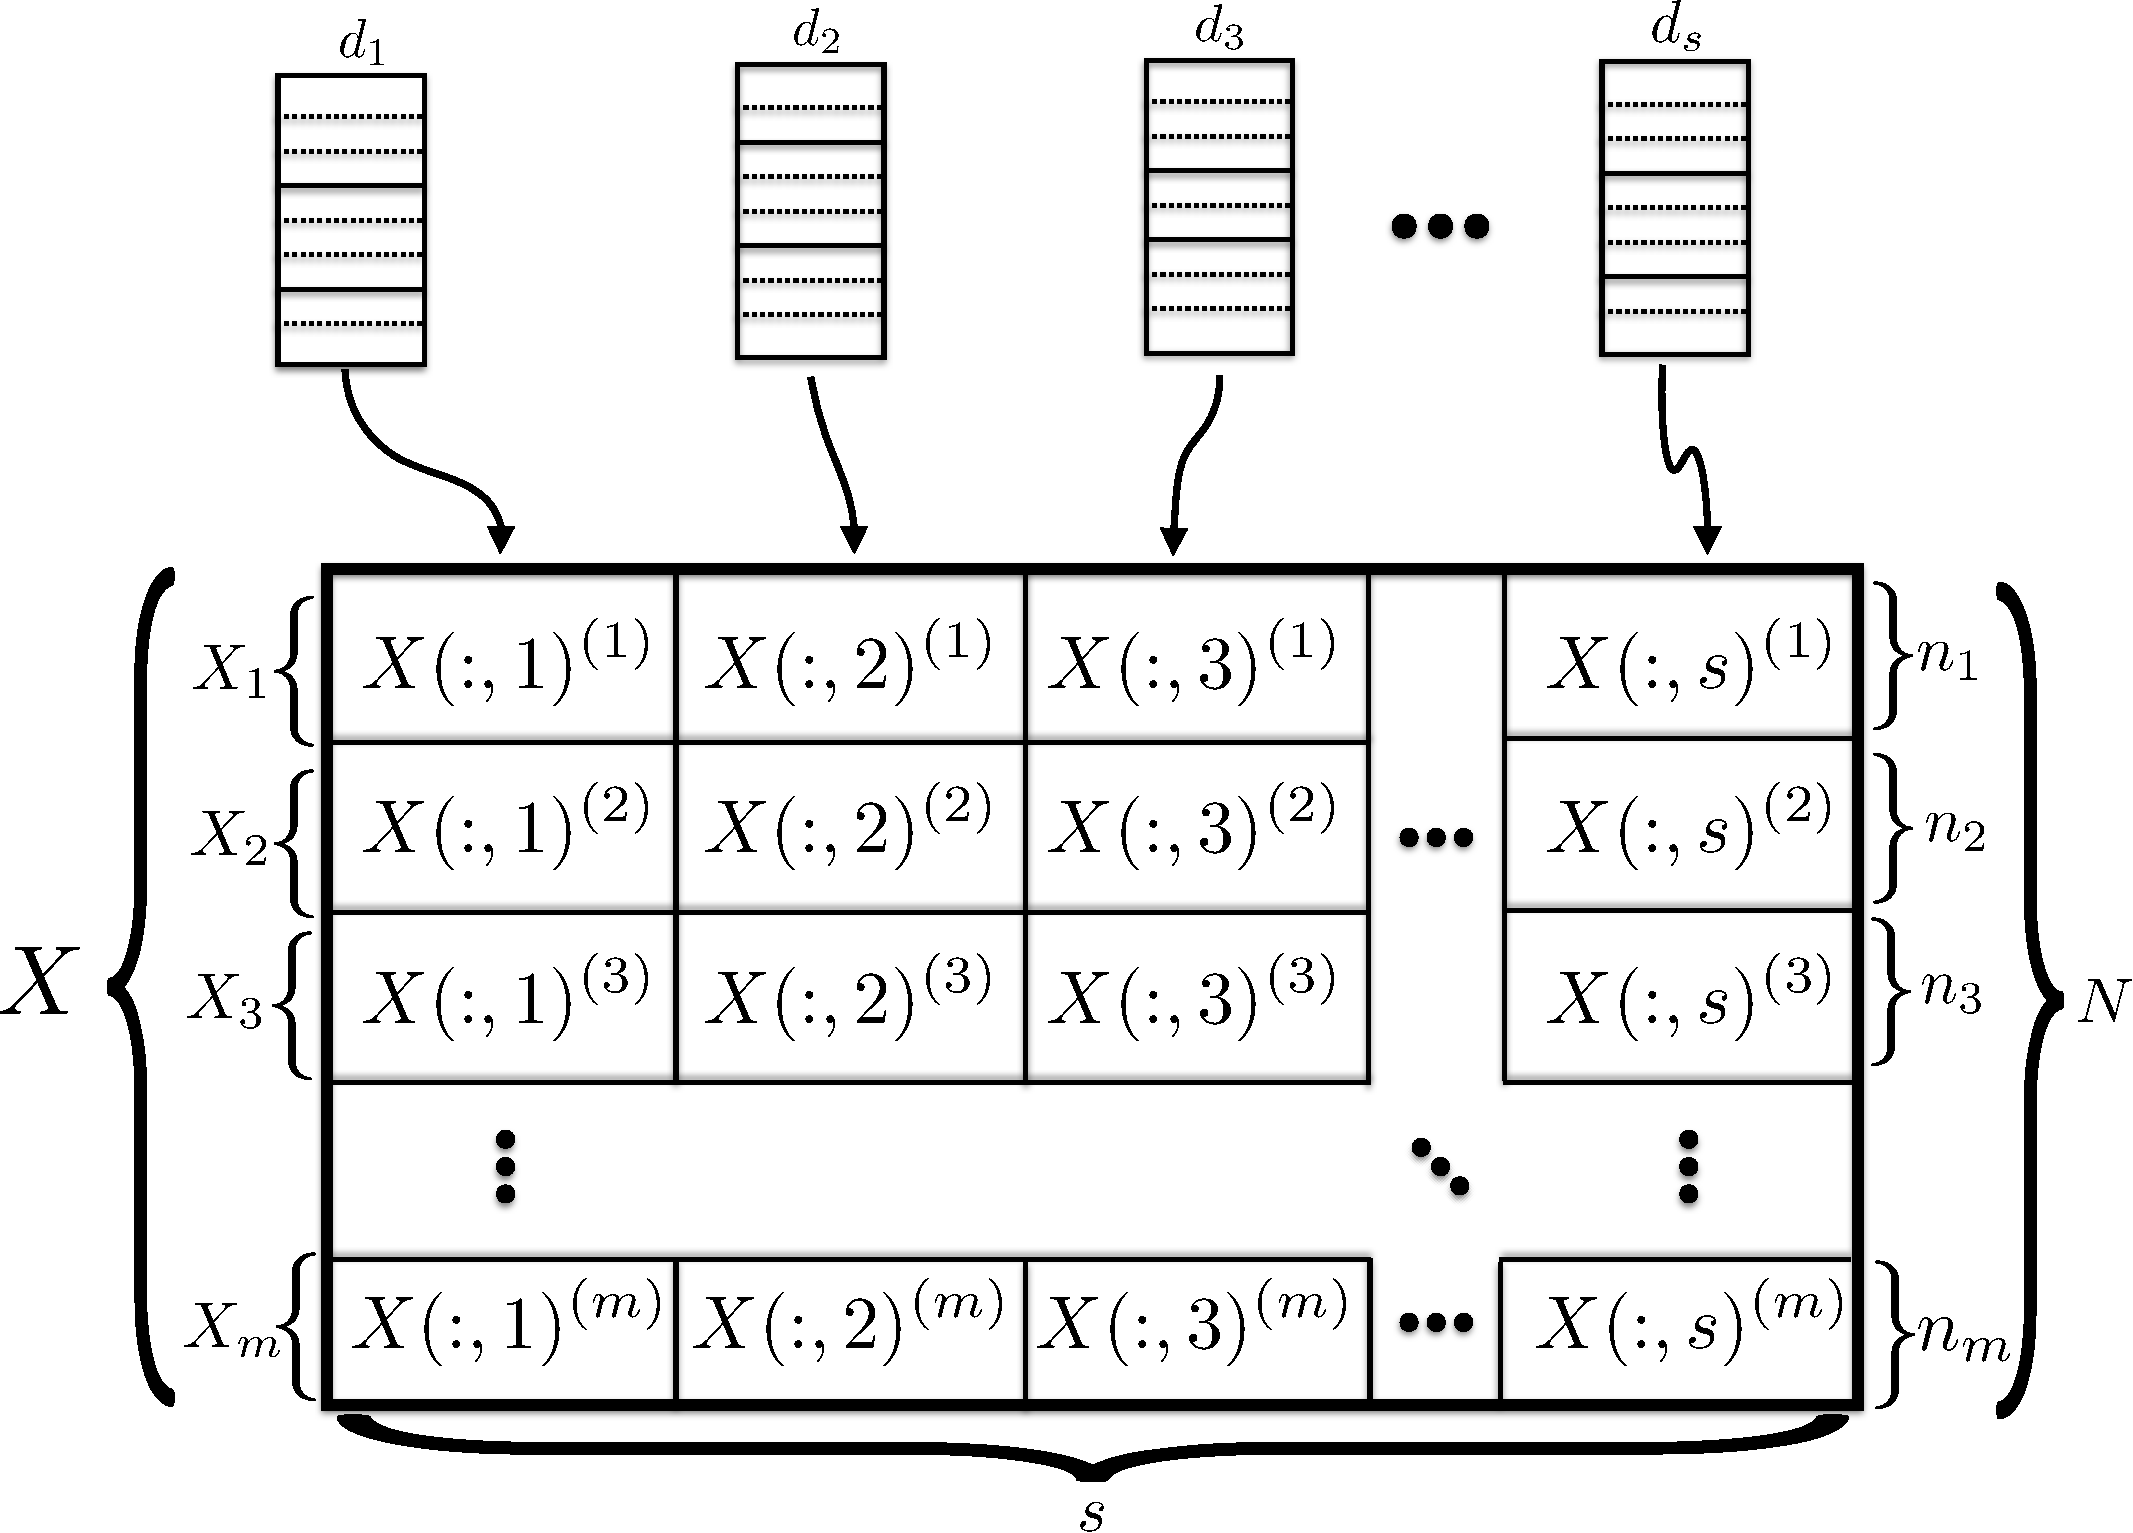
\includegraphics[width=9cm]{figures/stacked_matrices1-crop.pdf}
\caption[Multilingual corpus matrices]{Multilingual corpora and their matrix representations using the vector space model.}
\label{fig:stacked_matrices}
\end{figure}

We will now describe four models to cross-lingual similarity computation, where the first three are based on
methods introduced in Chapter~\ref{chap:background} and the fourth one represents an original contribution.
\section{$k$-means}\label{chap:crosslingual:kmeans}

We have introduced the $k$-means algorithm in Section~\ref{chap:background:kmeans} and we now discuss
how to apply it to build a cross-lingual similarity function. In a nutshell, we apply the standard
$k$-means procedure to the stacked multiview matrix and interpret the centroids as an aligned basis, which
is used to build the CL-similarity model; see Figure~\ref{fig:kmeans} for an illustration of the approach.

\begin{figure}[tbp]
\centering
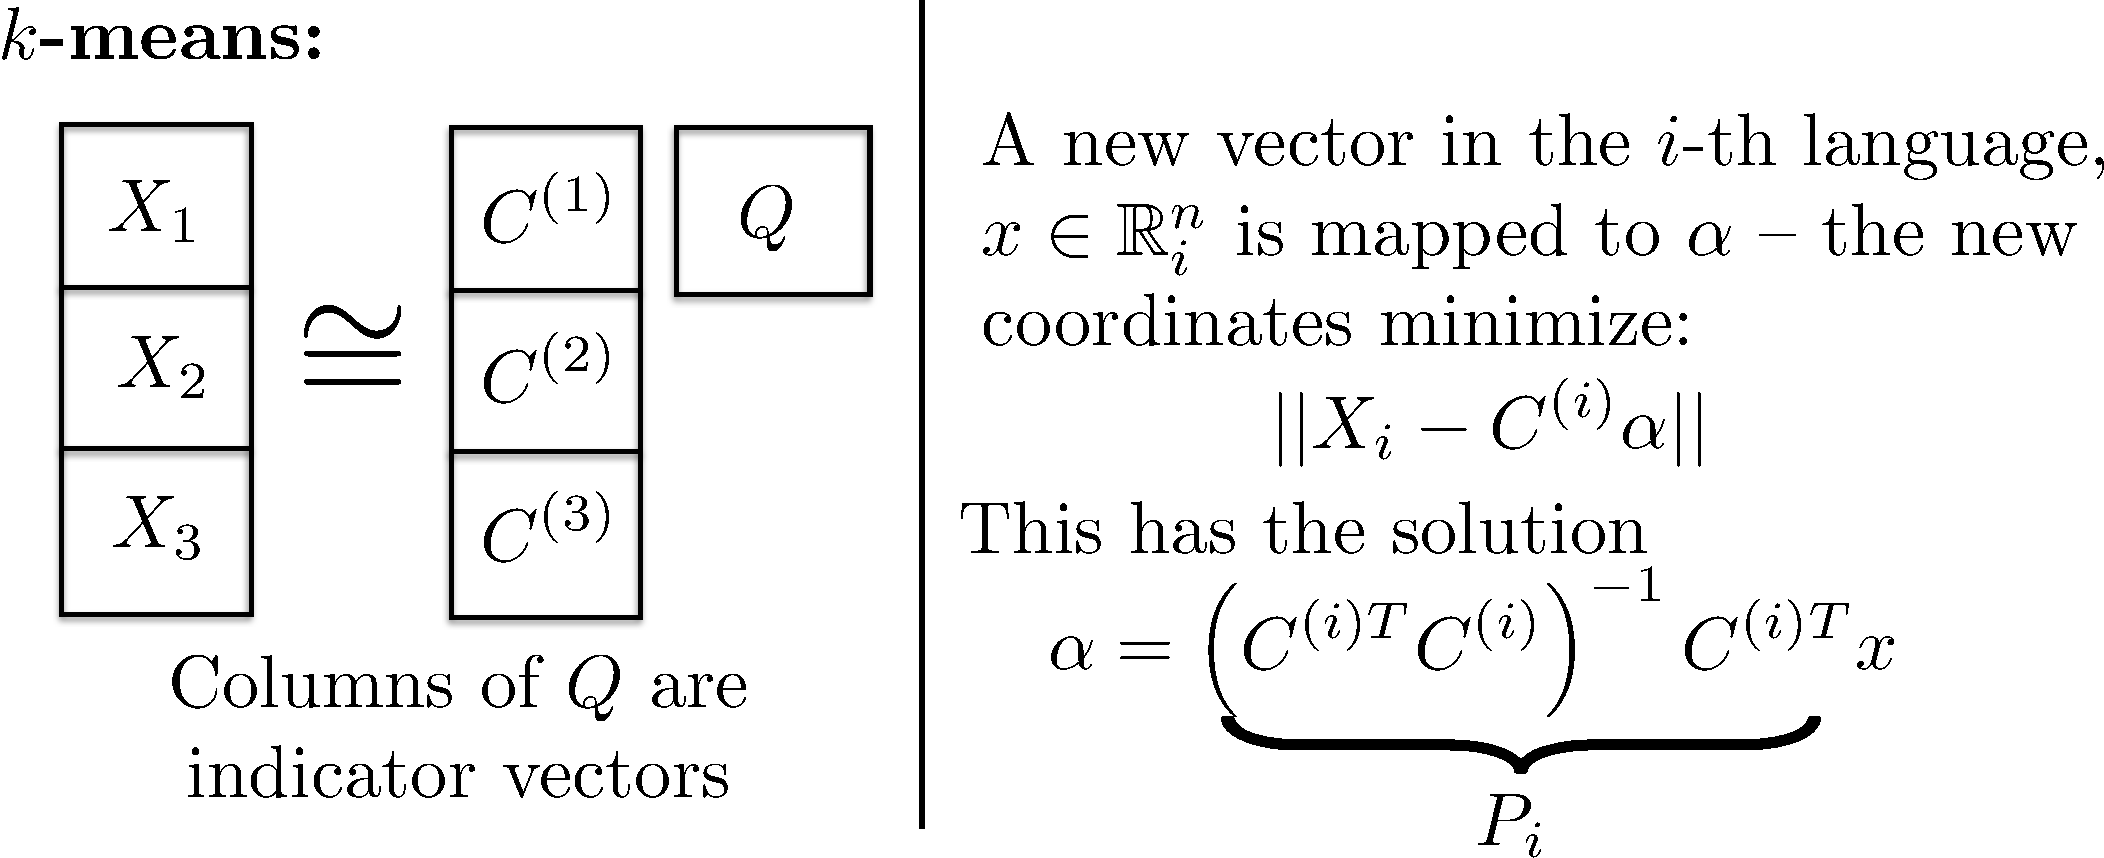
\includegraphics[width=10cm]{figures/kmeans.pdf}
\caption{$k$-means algorithm and coordinate change.}
\label{fig:kmeans}
\end{figure}

In order to apply the algorithm, we first merge all the term-document matrices into a single matrix
$X$ by stacking the individual term-document matrices (as seen in Figure~\ref{fig:stacked_matrices}):
$$X := \begin{bmatrix}X_1^T ,X_2^T, \cdots, X_m^T \end{bmatrix}^T,$$
such that the columns respect the alignment of the documents (here MATLAB notation for concatenating
matrices is used). Therefore, each document is represented by a long vector indexed by the terms in all languages.

We then run the $k$-means algorithm and obtain a centroid matrix $C \in \RR^{N \times k}$,
where the $k$ columns represent centroid vectors. The centroid matrix can be split vertically into $m$
blocks: $$C = [C^{(1)T} \cdots C^{(m^T)}]^T,$$ according to the number of dimensions of each language,
i.e., $C^{(i)} \in \RR^{n_i \times k}$.

To reiterate, the matrices $C^{(i)}$ are computed using a multilingual corpus
matrix $X$ (based on Wikipedia for example).

To compute  cross-lingual document similarities on new documents, we interpret each matrix $C^{(i)}$
as a vector space basis which can be used to map points in $\RR^{n_i}$ into a $k$-dimensional space. Given
a new vector $x \in \RR^{n_i}$ we can express its coordinates as:
$$(C^{(i)T} C^{(i)})^{-1} C^{(i)T} x_i.$$

The resulting matrix for similarity computation between language $i$ and language $j$
is defined up to a scaling factor as:
$$C^{(i)}(C^{(i)T} C^{(i)})^{-1} (C^{(j)T} C^{(j)})^{-1} C^{(j)T}.$$

The matrix is a result of mapping documents in a language independent space using
pseudo-inverses of the centroid matrices $P_i = (C^{(i)T} C^{(i)})^{-1} C^{(i)T}$ and then
comparing them using the standard inner product, which results in the matrix
$P_i^T P_j$. For the sake of presentation, we assumed that the centroid vectors
are linearly independent. (An independent subspace could be obtained using an
additional Gram-Schmidt step~\cite{golub} on the matrix $C$, if this was not the case.)

\section{Cross-Lingual Latent Semantic Indexing}\label{chap:crosslingual:LSI}

Section~\ref{chap:background:svd} introduced two closely related approaches
to pattern analysis based on spectral decompositions. This section summarizes
how these approaches apply to cross-lingual document analysis. Truncated Singular
value Decomposition (TSVD) applied to monolingual document analysis was introduced
in~\cite{lsi} where it is referred to as Latent Semantic Indexing (LSI). An extension
to cross-lingual document analysis was proposed in~\cite{cl_lsi} and is referred to as
Cross-Lingual Latent Semantic Indexing (CL-LSI). Now follows a description of a
variation of CL-LSI, relevant to the thesis.

The method is based on computing a truncated singular value decomposition of
multiview stacked matrix $X \approx U S V^T$. See Figure~\ref{fig:lsi} for the decomposition.
Representing documents in ``topic'' coordinates is done in the same way as in the $k$-means case
(see Figure~\ref{fig:kmeans}), we will describe how to compute the coordinate change functions.

\begin{figure}[tbp]
\centering
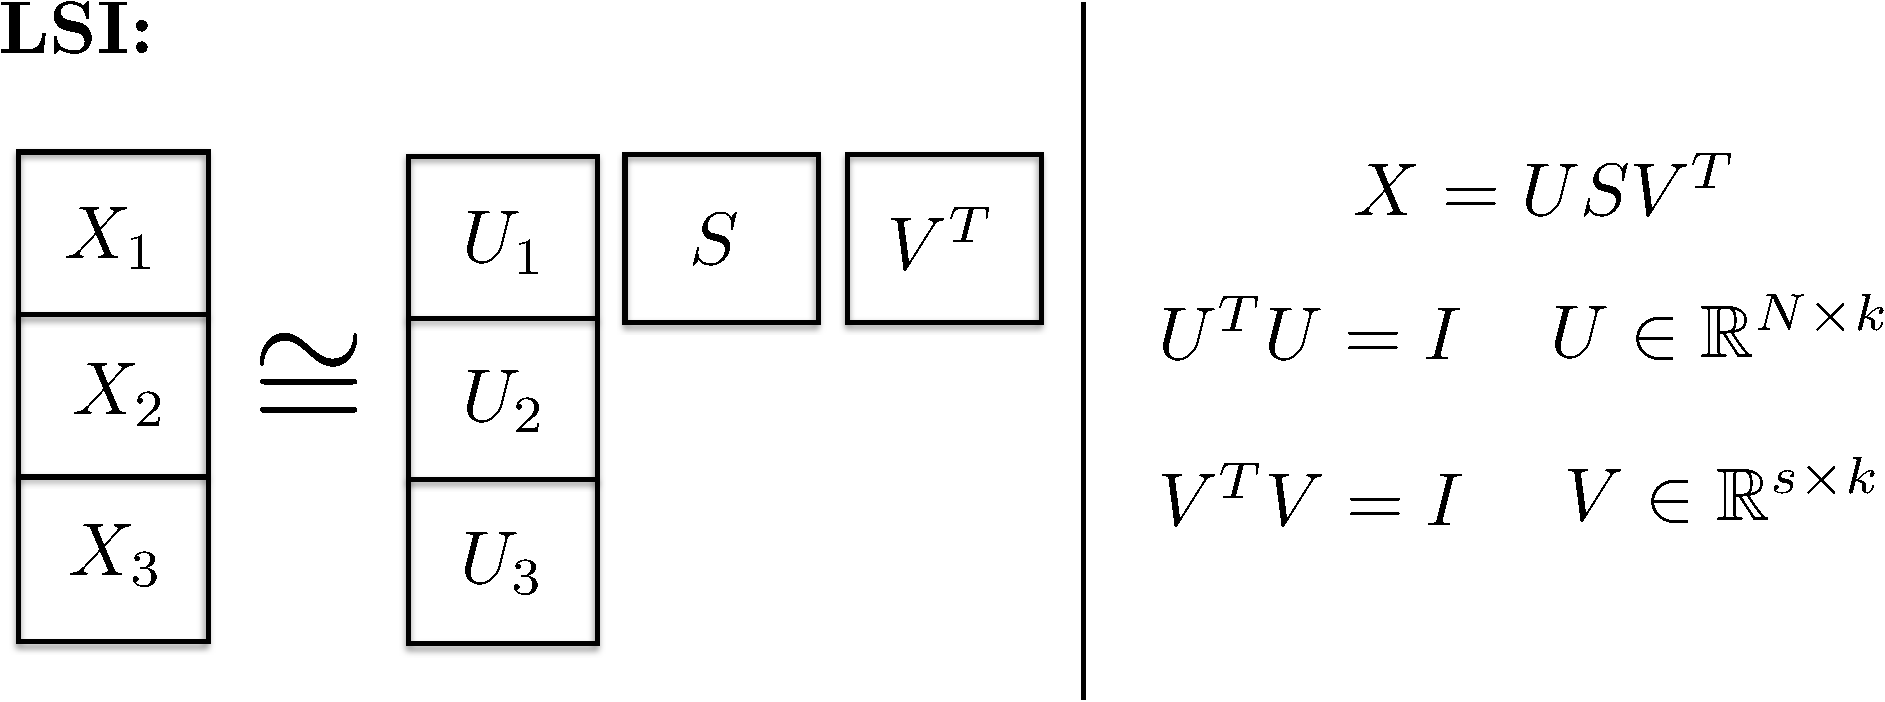
\includegraphics[width=10cm]{figures/lsi.pdf}
\caption{LSI multilingual corpus matrix decomposition.}
\label{fig:lsi}
\end{figure}

The cross-lingual similarity functions are based on a rank-$k$ truncated SVD:
$X \approx U \Sigma V^T,$ where $U \in \RR^{N \times k}$ are basis vectors of
interest and $\Sigma \in \RR^{k \times k}$ is a truncated diagonal matrix of singular
eigenvalues. An aligned basis is obtained by first splitting $U$ vertically according
to the number of dimensions of each language: $U = [U^{(i)T} \cdots U^{(m)T}]^T$.
The standard CL-LSI approach is to use matrices $U_i$ directly as maps to the common
coordinate space - the cross-lingual similarity function between two documents $x_i$ and
$x_j$ is given by $x_i^T U^{(i)} S^{-1} S^{-1} U^{(j)T} x_j$. We note that in general the blocks
are not orthogonal and the norms of their columns may vary. Our modification to the
standard approach is to treat $U^{(i)}$ as aligned bases, and use their pseudo-inverses
to construct projection maps (exactly $k$-means centroids were treated). Assuming
that the blocks $X^{(i)}$ have full rank (and thus so are $U^{(i)}$), 
the pseudo-inverses can be expressed as $P_i := (U^{(i)T} U^{(i)})^{-1} U^{(i)T}$.
The matrices $P_i$ are used to change the basis from the standard basis in $\RR^{n_i}$ to the
basis spanned by the columns of $U_i$.

\bolded{Implementation note.}
Since the matrix $X$ can be large we could use an iterative method like the Lanczos
algorithm with re-orthogonalization~\cite{golub} to find the left singular vectors
(columns of $U$) corresponding to the largest singular values. In our experiments
the Lanczos method converged slowly indicating problems with singular value separation. 
Moreover, the Lanczos method is hard to parallelize. Instead, we use a randomized version
of the SVD~\cite{tropp} that can be viewed as a block Lanczos method. That enables us
to use parallelization and speeds up the computation considerably.

To compute the matrices $P_i$ we used the QR algorithm~\cite{golub} to factorize
$U^{(i)}$ as $U^{(i)} = Q_i R_i$, where $Q_i^TQ_i = I$ and $R_i$ is a triangular matrix.
$P_i$ is then obtained by solving $R_i P_i = Q_i$.

\section{Bi-Lingual Document Analysis CCA}\label{chap:crosslingual:CCA}
CCA can be applied to bi-lingual document analysis given two languages. Let $X_1 \in \RR^{p \times \ell}$
and $X_2 \in ^{q \times \ell}$ denote the two multiview aligned matrices based on a bi-lingual aligned
document collection vectorized using two vector space models.
If $W^{(1)}\in \RR^{p\times k}$ and $W^{(2)} \in \RR^{q\times k}$ are solutions comprising of $k$ canonical
correlation vector pairs (corresponding to columns of $W^{(1)}$ and $W^{(2)}$)
of the generalized eigenvalue problem in Equation~\ref{eq:background:cca:eigen}, then
the bi-lingual similarity function that we use is expressed as a cosine similarity
after applying the canonical maps:
$$\textnormal{sim}(x_1, x_2) \propto \frac{x_1^T W^{(1)}W^{(2)^T}x_2}{\norm{W^{(1)T}x_1} \norm{W^{(2)T}x_2}} .$$
The intuition behind using the matrices as projectors (even though their columns are not an
orthonormal basis) is that the CCA is equivalent to minimizing the expected
distance between $W^{(1)T}\mathcal{X}^{(1)}$ and $W^{(2)T}\mathcal{X}^{(2)}$,
see Section 6.5 in~\cite{shawe-taylor04kernel}.


\section{Hub Language Based CCA Extension}\label{chap:crosslingual:hublang}
Building cross-lingual similarity models based on comparable corpora is challenging for
two main reasons. The first problem is related to missing alignment data: when a number
of languages is large, the dataset of documents that cover all languages is small (or may
even be empty). Even if only two languages are considered, the set of aligned documents
can be small (an extreme example is given by the Piedmontese and Hindi Wikipedias where
no inter-language links are available), in which case none of the methods presented so
far are applicable.

The second challenge is scale - the data is high-dimensional (many languages with
hundreds of thousands of features per language) and the number of multilingual documents may
be large (over one million in case of Wikipedia). The optimization problem posed by CCA is not trivial
to solve: the covariance matrices themselves are prohibitively
large to fit in memory (even storing a 100,000 by 100,000 element matrix requires
80GB of memory) and iterative matrix-multiplication based approaches to solving generalized
eigenvalue problems are required (the covariance matrices can be expressed as products
of sparse matrices, which means we have fast matrix-vector multiplication).

We now describe an extension of CCA to more than two languages, which can be trained on
large comparable corpora and can handle missing data. The extension we consider is based on
a generalization of CCA to more than two views, introduced in~\cite{Kettenring}, namely
the Sum of Squared Correlations SSCOR, introduced in Equation~\ref{eq:SSCOR} in
Section~\ref{chap:extensions:sumcor}, which we will re-state formally later in this section.
Our approach exploits a certain characteristic of the data, namely the \emph{hub language}
characteristic (see below) in two ways: to reduce the dimensionality of the data and to
simplify the optimization problem. We focus on the SSCOR formulation as opposed to the SCOR
formulation which we explored in the previous chapters, since the Lagrangian problem is easier
to solve (That is under the hub language assumption, which we present next).

\bolded{Hub language characteristic.}
In the case of Wikipedia, we observed that even though the training resources are scarce
for certain language pairs, there often exists indirect training data. By considering
a third language, which has training data with both languages in the pair,  we can use
the composition of learned maps as a proxy. We refer to this third language as a hub language.

A \emph{hub language} is a language with a high proportion of non-empty documents in
$D = \left\{d_1,..., d_{\ell}\right\}$. As we have mentioned, we only focus on multilingual
documents that include at least two languages. The prototypical example in the case of
Wikipedia is English. Our notion of the hub language could be interpreted in the following
way. If a non-English Wikipedia page contains one or more links to variants of the page in
other languages, English is very likely to be one of them. That makes English a hub language.

We use the following notation to define subsets of the multilingual comparable corpus:
let $a(i,j)$ denote the index set of all multilingual documents with non-missing data
for the $i$-th and $j$-th language:
$$a(i,j) = \left\{k~ |~ d_k = (u_1,...,u_m), u_i \neq \emptyset, u_j \neq \emptyset \right\},$$
and let $a(i)$ denote the index set of all multilingual documents with non missing data
for the $i$-th language.

We now describe a two step approach to building a cross-lingual similarity matrix.
The first part is related to LSI and reduces the dimensionality of the data. The second
step refines the linear mappings and optimizes the linear dependence between data.

\bolded{Step 1: Hub language based dimensionality reduction.}
The first step in our method is to project $X_1, \ldots, X_m$ to lower-dimensional spaces
without destroying the cross-lingual structure. Treating the nonzero columns of $X_i$ as
observation vectors sampled from an underlying distribution $\mathcal{X}^{(i)} \in \RR^{n_i}$,
we can analyze the empirical cross-covariance matrices:
$$C^{(i,j)} = \frac{1}{|a(i,j)|-1 }\sum_{\ell \in a(i,j)} (X_i(:,\ell) - c_i)\cdot (X_j(:,\ell) - c_j)^T,$$
where $c_i = \frac{1}{|a_i|} \sum_{\ell \in a(i)}X_i(:,\ell)$. By finding low-rank
approximations of $C^{(i,j)}$ we can identify the subspaces that are
relevant for extracting linear patterns between $\mathcal{X}^{(i)}$ and $\mathcal{X}^{(j)}$.
Let $X_1$ represent the hub language corpus matrix. The LSI approach to finding the subspaces
is to perform the singular value decomposition on the full $N \times N$ covariance matrix
composed of blocks $C^{(i,j)}$. If $|a(i,j)|$ is small for many language pairs (as it is in the
case of Wikipedia), then many empirical estimates $C^{(i,j)}$ are unreliable, which can result
in overfitting. For this reason, we perform the truncated singular value decomposition on the
matrix $C = [C^{(1,2)}  \cdots  C^{(1,m)}] \approx U S V^T$, where
$U \in \RR^{n_1 \times k}, S \in \RR^{k \times k}, V \in \RR^{(\sum_{i=2}^m n_i) \times k}$.
Define $T = [U^T V^T]^T \in \RR^{N \times k}$, which is compatible with the block structure $b = (n_1, \ldots, n_m)$.
Note that the columns of $T^{(1)}$ are orthonormal, but that is not true in general for the other blocks.
We proceed by reducing the dimensionality of each $X_i$ by
setting: $Y_i = T^{(i)T} \cdot X_i$, where $Y_i \in \RR^{k\times s}$. To summarize, the first step
reduces the dimensionality of the data and is based on CL-LSI, but optimizes only the hub language
related cross-covariance blocks.

\bolded{Step 2: Simplifying and solving SSCOR.}
The second step involves solving a generalized version of canonical correlation analysis on the
matrices $Y_i$ in order to find the mappings $P_i$. The approach is based on the sum of
squares of correlations formulation by Kettenring~\cite{Kettenring}, where we consider only
correlations between pairs $(Y_1, Y_i), i >1$ due to the hub language problem characteristic.
We will present the original unconstrained optimization problem, then a constrained formulation
based on the hub language problem characteristic. Then we will simplify the constraints and
reformulate the problem as an eigenvalue problem by using Lagrange multipliers.

The original sum of squared correlations is formulated as an unconstrained problem:
\begin{equation*}
  \begin{aligned}
    & \underset{w_i \in \RR^{k}}{\text{maximize}}
    & & \sum_{i < j}^m  \rho(w_i^T Y_i, w_j^T Y_j)^2.
\end{aligned}
\end{equation*}
We solve a similar problem by restricting $i=1$ and omitting the optimization over non-hub
language pairs. Let $D_{i,i} \in \RR^{k \times k}$ denote the empirical covariance of
$\mathcal{Y}_i$ and $D_{i,j}$ denote the empirical cross-covariance computed based on
$\mathcal{Y}_i$ and $\mathcal{Y}_j$. We solve the following constrained (unit variance
constraints) optimization problem:
\begin{equation}\label{squaredCorHubOriginal}
  \begin{aligned}
    & \underset{w_i \in \RR^{k}}{\text{maximize}}
    & & \sum_{i = 2}^m  \left(w_1^T D_{1,i} w_i \right)^2
    & \text{subject to}
    & & w_i^T D_{i,i} w_i = 1, \quad\forall i = 1,\ldots, m.
\end{aligned}
\end{equation}
The constraints $w_i^T D_{i,i} w_i$ can be simplified by using the Cholesky decomposition
$D_{i,i} = K_i^T \cdot K_i$ and substitution: $y_i := K_i w_i$. By inverting the $K_i$
matrices and defining  $G_i := K_1^{-T} D_{1,i} K_i^{-1}$, the problem can be reformulated:
\begin{equation}\label{squaredCorHub}
  \begin{aligned}
    & \underset{y_i \in \RR^{k}}{\text{maximize}}
    & & \sum_{i = 2}^m  \left(y_1^T G_{i} y_i \right)^2
    & \text{subject to}
    & & y_i^T y_i = 1, \quad\forall i = 1,\ldots, m.
\end{aligned}
\end{equation}
A necessary condition for optimality is that the derivatives of the Lagrangian vanish.
The Lagrangian of (\ref{squaredCorHub}) is expressed as:
$$  L(y_1, \ldots, y_m, \lambda_1, \ldots, \lambda_m) =
\sum_{i = 2}^m  \left(y_1^T G_{i} y_i \right)^2 + \sum_{i=1}^m \lambda_i \left(y_i^T y_i - 1\right).$$
Stationarity conditions give us:
\begin{eqnarray}
 \label{dLdx1}  \frac{\partial}{\partial y_1} L = 0 & \Rightarrow & \sum_{i = 2}^m  \left(y_1^T G_{i} y_i \right) G_i y_i + \lambda_1 y_1 = 0, \\
 \label{dLdxi} \frac{\partial}{\partial y_i} L = 0 & \Rightarrow & \left(y_1^T G_{i} y_i \right) G_{i}^T y_1 + \lambda_i y_i = 0,~i > 1.
\end{eqnarray} 
Multiplying each Equation (\ref{dLdxi}) with $y_i^T$ and applying the
constraints, we can eliminate $\lambda_i$ which gives us:
\begin{equation}\label{eqy1yi}
G_{i}^T y_1 = \left(y_1^T G_{i} y_i \right) y_i,~i > 1.
\end{equation}
Plugging this into Equation (\ref{dLdx1}), we obtain an eigenvalue problem:
$$\left( \sum_{i = 2}^m G_i G_{i}^T \right) y_1 + \lambda_1 y_1 = 0.$$
The eigenvectors of $\left( \sum_{i = 2}^m G_i G_{i}^T \right)$ solve
the problem for the first language. The solutions for $y_i$ are obtained
from (\ref{eqy1yi}): $y_i := \frac{G_{i}^T y_1}{\| G_{i}^T y_1 \|}$.
Note that the solution (\ref{squaredCorHubOriginal}) can be recovered
by: $w_i := K_i^{-1} y_i$. The original variables $w$
are then expressed as:
\begin{eqnarray} 
Y_1 & := & \text{eigenvectors of}~\sum_{i = 2}^m G_i G_{i}^T,\\
W_1 &  = & K_1^{-1} Y_1,\\
W_i &  = & K_i^{-1} G_{i}^T Y_1 N,
\end{eqnarray}
where $N$ is a diagonal matrix that normalizes $G_{i}^T Y_1$, with
$N(j,j) := \frac{1}{\|G(_{i} Y_1(:,j)\|}$.

\bolded{Remark.} The technique is related to  Generalization of Canonical
Correlation Analysis (GCCA)~\cite{Carroll}, where an unknown
group configuration variable is defined and the objective is to maximize the
sum of squared correlations between the group variable and the others. The
problem can be reformulated as an eigenvalue problem. The difference lies in
the fact that we set the unknown group configuration variable as the hub language,
which simplifies the solution. The complexity of our method is $O(k^3)$, where $k$
is the reduced dimension from the LSI preprocessing step, whereas solving the
GCCA method scales as $O(s^3)$, where $s$ is the number of samples (see~\cite{gifi}).
Another issue with GCCA is that it cannot be directly applied to the case of missing documents.

To summarize, we first reduced the dimensionality of our data to $k$-dimensional
features and then found a new representation (via linear transformation) that
maximizes directions of linear dependence between the languages. The final
projections that enable mappings to a common space are defined as:
$P_i(x) := W_i^T T^{(i)T} x.$

\bolded{Remark on SUMCOR.}
The original sum of correlations is formulated as an unconstrained problem:
\begin{equation*}
  \begin{aligned}
    & \underset{w_i \in \RR^{k}}{\text{maximize}}
    & & \sum_{i < j}^m  \rho(w_i^T Y_i, w_j^T Y_j).
\end{aligned}
\end{equation*}
Under the hub language assumption, this problem is equivalent to (analogous to how we derived the formulation in Equation \ref{squaredCorHub}):
\begin{equation}\label{sumCorHub}
  \begin{aligned}
    & \underset{y_i \in \RR^{k}}{\text{maximize}}
    & & \sum_{i = 2}^m  y_1^T G_{i} y_i \\
    & \text{subject to}
    & & y_i^T y_i = 1, \quad\forall i = 1,\ldots, m.
\end{aligned}
\end{equation}
The Lagrangian of (\ref{sumCorHub}) is expressed as:
$$  L(y_1, \ldots, y_m, \lambda_1, \ldots, \lambda_m) =
\sum_{i = 2}^m  y_1^T G_{i} y_i + \sum_{i=1}^m \lambda_i \left(y_i^T y_i - 1\right).$$
Stationarity conditions give us:
\begin{equation}
\begin{aligned} \label{SUMCORdLdx}
  \frac{\partial}{\partial y_1} L = 0 \quad \Rightarrow \quad  &~ \sum_{i = 2}^m  G_i y_i + \lambda_1 y_1 =  0,& \\
  \frac{\partial}{\partial y_i} L = 0 \quad \Rightarrow \quad &~ G_{i}^T y_1 + \lambda_i y_i = 0,&\quad i > 1. \\
\end{aligned}
\end{equation}
%Multiplying Equations (\ref{SUMCORdLdx}) by $y_i$ and using the constraints one can express $\lambda_i$ as:
%\begin{equation}
%\begin{aligned}
%& \lambda_1 & = & - \sum_{i = 2}^m  y_1^T G_i y_i, &\\
%& \lambda_i & = & - y_i^T G_{i}^T y_1, &\quad i > 1.\\
%\end{aligned}
%\end{equation}
It follows that:
$$
G_i y_i = -\frac{1}{\lambda_i} G_i G_i^T y_1,
$$
and thus:
$$
\sum_{i = 2}^m -\frac{1}{\lambda_i} G_i G_i^T y_1 + \lambda_1 y_1 = 0.
$$
Since the following equality can be derived: 
$$\lambda_1 = \sum_{i = 2}^m \lambda_i$$ 
the original problem reduces to
$$
\sum_{i = 2}^m -\frac{1}{\lambda_i} G_i G_i^T y_1 + \sum_{i=2}^m \lambda_i y_1 = 0,
$$
but the solution to that problem does not seem obvious. This is in contrast to the SSCOR problem, where all $\lambda_i$ as
well as $y_i$ could be eliminated simultaneously.

\vspace{5mm}
\bolded{Summary.}
This chapter presented the problem of computing cross-lingual document similarities and then presented four computational
approaches to solve the problem. The last one is an original contribution of the author and is based on combining an efficient
preprocessing step with a particular generalization of CCA (SSCOR), which under an additional assumption (hub language) can
be solved efficiently (both the preprocessing step as well as the simplifying assumption are crucial for the approach). The
next chapter will discuss how the cross-lingual similarity function can be used in a large scale cross-lingual news analysis system.
%--------------------------------------------------------------------------------------------------
%
\chapter{Applications to Cluster Linking}\label{chap:applications}
%--------------------------------------------------------------------------------------------------

In online media streams -- particularly news articles -- there is often duplication of reporting,
different viewpoints or opinions, all centering around a single event. Typically each event is covered by many articles
and the question we address is how to find all the articles in different languages that are reporting on the same event.
The current chapter describes an application of the cross-lingual similarity presented in Chapter~\ref{chap:crosslingual}
to cross-lingual cluster linking. The application is relevant for monitoring global news in multiple languages.
Presented in the current chapter is our original approach to cross-lingual cluster linking,
which was published in~\cite{rupnikJAIR}. The main idea in our approach is to combine
semantic information extraction with cross-lingual document analysis, which we proved to be
effective in~\cite{Belyaeva201564}. There we used a simpler set of features to
decide which clusters to link and put greater emphasis on the manual evaluation of the quality.

To prepare the ground for the discussion of the cross-lingual approach, we will first
describe how \emph{events} are defined for our purposes and
sketch a general approach to event tracking in a monolingual setting.

The term event is vague and ambiguous, but for the practical purposes, we define
it as ``any significant happening that is being reported about in the media''.
Examples of events would include shooting down of the Malaysia Airlines plane over
Ukraine on July 18th, 2014 (see Figure~\ref{fig:event2}) and HSBC's admittance of
aiding their clients in tax evasion on February 9th, 2015. Events such as these are
covered by many articles and the question is how to find all the articles in
different languages that are describing a single event. Generally, events are more
specific than general themes as the time component plays an important role --
for example, the two wars in Iraq would be considered as separate events.

\begin{figure}
\centering
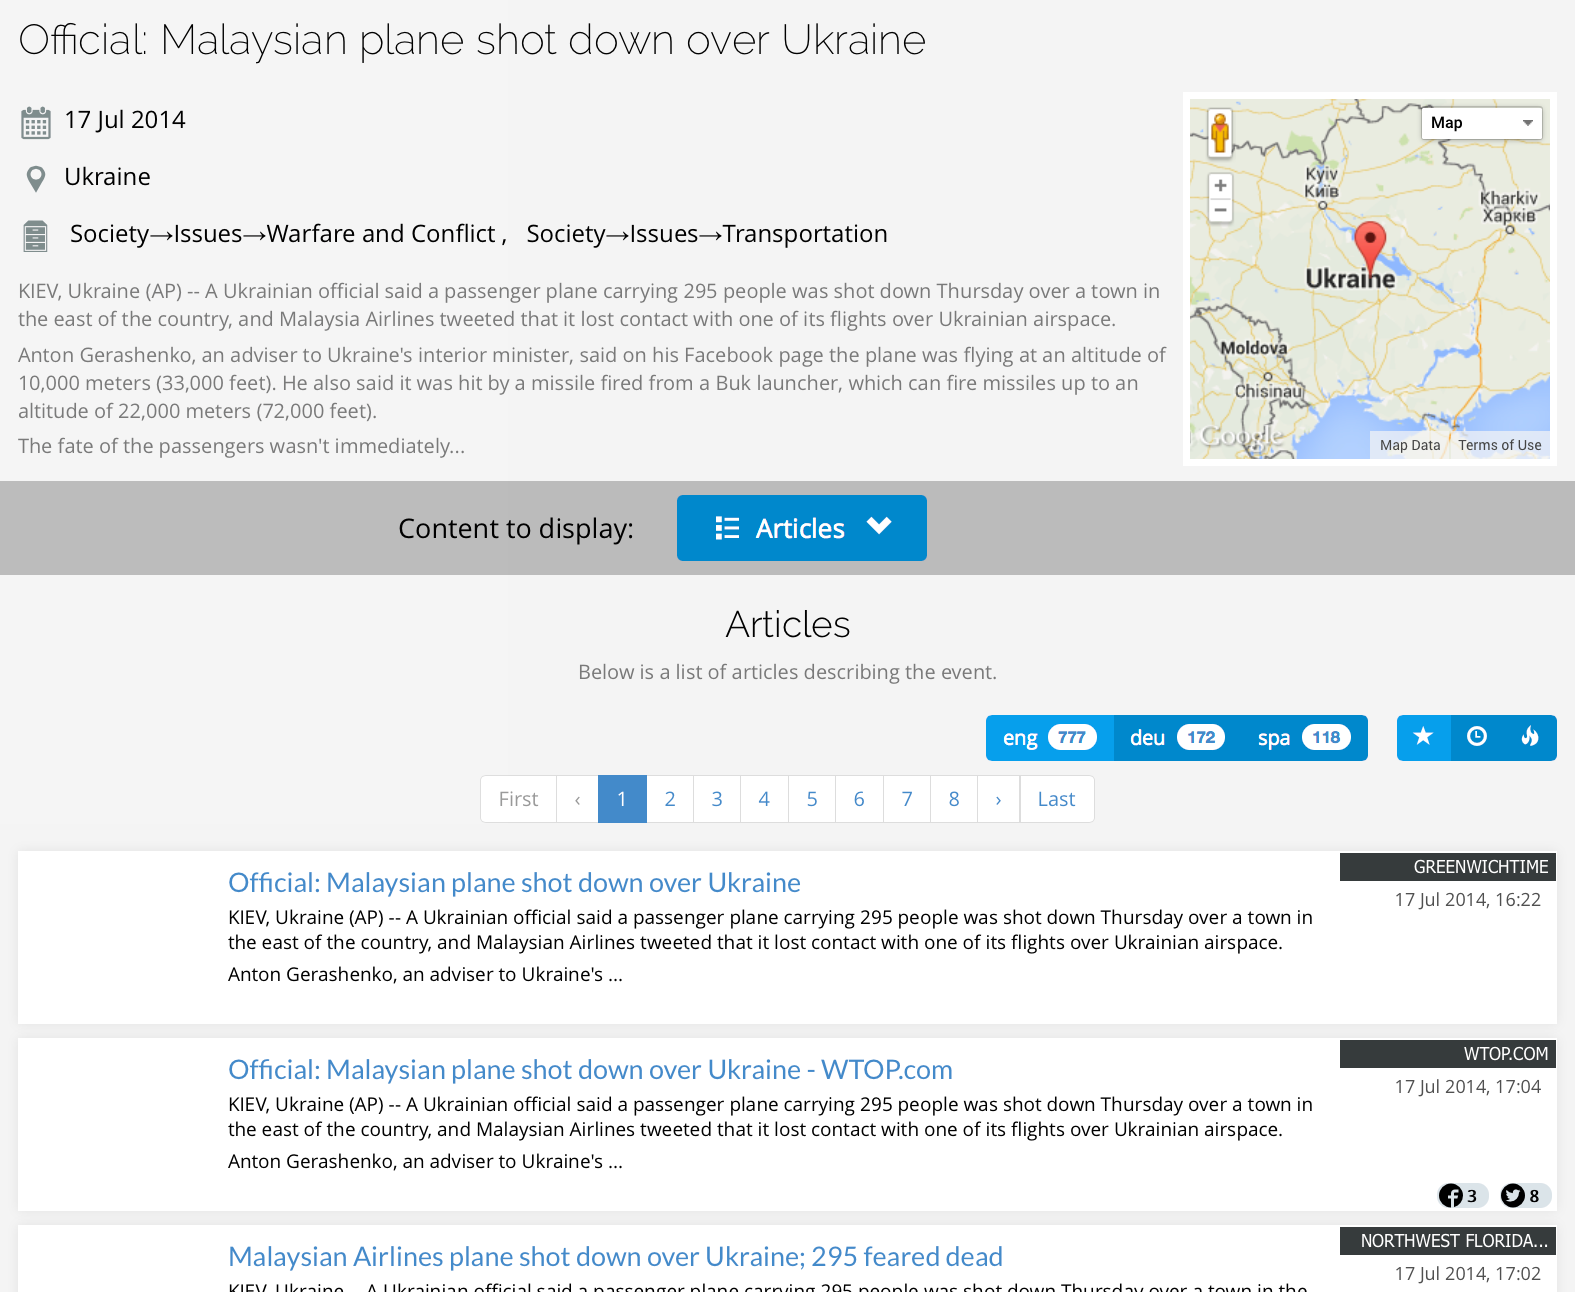
\includegraphics[width=1\textwidth]{figures/events2.png}
\caption{\label{fig:event2} Events are represented by collections of articles about an event, in
this case the Malaysian airliner which was shot down over Ukraine. The results shown in the figure can be obtained using the query \url{http://eventregistry.org/event/997350\#?lang=eng\&tab=articles}. The
content presented is part of the Event Registry system, developed by the authors.}
\end{figure}


We take a pragmatic approach where the events are \textbf{identified} as the clusters
discovered by stream clustering algorithm that is designed to cluster
news articles together if their content is similar and they are published
close in time.

The particular choice of a streaming clustering algorithm is not relevant
to the discussion of our approach and we assume that given a monolingual news stream, we have
at our disposal an online clustering component which assigns to each news
article a cluster ID. In this work we used the clustering
component of the Event Registry~\cite{Leban2014W}~and~\cite{Leban2014I} system.

We now consider the case where we are dealing with several document streams, where each
stream corresponds to a particular language. Running the monolingual streaming clustering
on each stream results in clusters within streams that need to be matched across streams,
which we will state formally.

\section{Problem Definition}

The problem of cross-lingual event linking is to match monolingual clusters of news articles
that are describing the same event across languages. For example, we want to match a cluster of
Spanish news articles and a cluster of English news articles that both describe the same earthquake.

Each article $a \in A$ is written in a language $\ell$, where $\ell \in L = \{\ell_1,\ell_2,...,\ell_m\}$.
For each language $\ell$, we obtain a set of monolingual clusters $C_{\ell}$. More precisely,
the articles corresponding to each cluster $c \in C_{\ell}$ are written in the language $\ell$.
Given a pair of languages $\ell_a \in L$, $\ell_b \in L$ and $\ell_a \not= \ell_b$, we would like
to identify all cluster pairs $(c_i, c_j) \in C_{\ell_a} \times C_{\ell_b}$ such that $c_i$ and $c_j$ describe the same event.

\begin{figure}[tb]
\centering
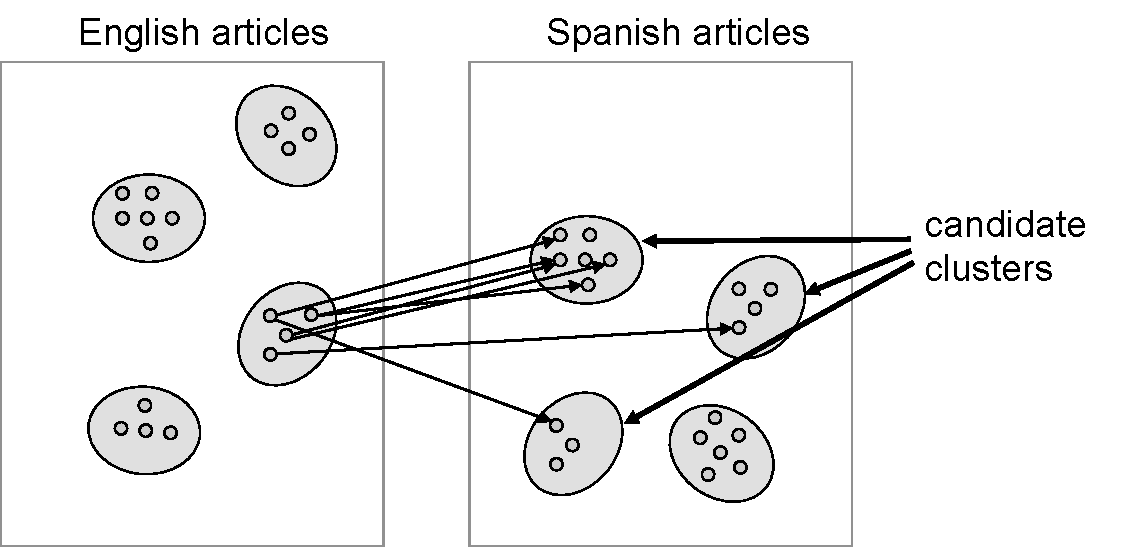
\includegraphics[width=0.7\textwidth]{figures/clusters.pdf}
\caption{\label{fig:clusters} Clusters composed of English and Spanish news articles. Arrows link English articles with their Spanish $k$-nearest neighbor matches according to the cross-lingual similarity.}
\end{figure}

Matching of clusters is a \emph{generalized matching} problem. We cannot assume that there is only
one cluster per language per event, nor can we assume complete coverage -- i.e., that there exists
at least one cluster per event in every language. This is partly due to news coverage which might
be more granular in some languages, partly due to noise and errors in the event detection process. This
implies that we cannot make assumptions on the matching (e.g., one-to-one or complete matching) and excludes
the use of standard weighted bipartite matching type of algorithms for this problem. An example is shown in
Figure~\ref{fig:clusters}, where a cluster may contain articles which are closely matched with many clusters in a different language.

We are also seeking for an algorithm which does not do exhaustive comparison of all clusters,
since that can become prohibitively expensive when working in a real-time setting. More specifically,
we wish to avoid testing cluster $c_i$ with all the clusters from all the other languages.
Performing exhaustive comparison would result in $O(|C|^2)$ tests, where $|C|$ is the number of all
clusters (over all languages), which is not feasible when the number of clusters is on the order of tens
of thousands. We address this by testing only clusters that are connected with at least one $k$-nearest
neighbor (marked as \emph{candidate clusters} in Figure~\ref{fig:clusters}).

\section{Algorithm}\label{algo:features}

In order to identify clusters that are equivalent to cluster $c_i$, we have developed
a novel two-stage approach. For a cluster $c_i$, we first efficiently identify a small set of
candidate clusters and then find those clusters among the candidates, which are
equivalent to $c_i$. An example is  shown in  Figure~\ref{fig:clusters}.

The details of the first step are described in Algorithm~\ref{cluster_merge_algo1}. The algorithm
begins by individually inspecting each news article $a_i$ in the cluster $c_i$. Using a chosen
method for computing cross-lingual document similarity (see Chapter~\ref{chap:crosslingual}), it identifies
the ten\footnote{This parameter was manually selected based on the storage and speed requirements of a real system.}
most similar news articles to $a_i$ in each language $\ell \in L$. For each similar
article $a_j$, we identify its corresponding  cluster $c_j$ and add it to the set of candidates.
The set of candidate clusters obtained in this way is several orders of magnitude smaller than the
number of all clusters, and at most linear with respect to the number of news articles in
cluster $c_i$. In practice, clusters contain highly related articles and as such similar
articles from other languages mostly fall in only a few candidate clusters.

Although computed document similarities are approximate, our  assumption is that articles
in different languages describing the same event will generally have a higher similarity
than articles about different events. While this assumption does not always hold, redundancy
in the data should mitigate these false positives.

\begin{algorithm}[t!]
\SetKwInput{KwInput}{input}\SetKwInput{KwOutput}{output}
\KwInput{test cluster $c_i$, a set of clusters $C_\ell$ for each language $\ell \in L$}
\KwOutput{a set of clusters $C$ that are potentially equivalent to $c_i$}
$C \leftarrow \{\}$\;
\For{article $a_i \in c_i$} {
    \For{language $\ell \in L$} {
        \tcc{use hub CCA to find 10 most similar articles to article $a_i$ in language $\ell$}
        $SimilarArticles = getCCASimilarArticles(a_i, \ell)$\;
        \For{article $a_j \in SimilarArticles$} {
            \tcc{find cluster $c_j$ to which article $a_j$ is assigned to}
            $c_j \leftarrow c$, such that $c \in C_\ell$ and $a_j \in c$\;
            \tcc{add cluster $c_j$ to the set of candidates $C$}
            $C \leftarrow C \cup \{ c_j \}$\;
        }
    }
}
\caption{Algorithm for identifying candidate clusters $C$ that are potentially equivalent to $c_i$}
\label{cluster_merge_algo1}
\end{algorithm}

The second stage of the algorithm determines which (if any) of the candidate clusters are equivalent to $c_i$.
We treat this task as a supervised learning problem. For each candidate cluster $c_j \in C$, we compute
a vector of learning features that should be indicative of whether $c_i$ and $c_j$ are equivalent or not
and apply a binary classification model that predicts if the clusters are equivalent or not. The classification
algorithm that we used to train a model was a linear Support Vector Machine (SVM) method~\cite{shawe-taylor04kernel}.

We use three groups of features to describe a cluster pair $(c_i, c_j)$. The first group is based
on {\bf cross-lingual article links}, which are derived using cross-lingual similarity:
each news article $a_i$ is linked with its $10$-nearest neighbors articles from all other
languages (ten per each language). The group contains the following features:

\begin{itemize}
\item \texttt{linkCount} is the number of times any of the news articles from $c_j$ is among $10$-nearest neighbors for articles from $c_i$. In other words, it is the number of times an article from $c_i$ has a very similar article (i.e., is among 10 most similar) in $c_j$.
\item \texttt{avgSimScore} is the average similarity score of the links, as identified for \texttt{linkCount}, between the two clusters.
\end{itemize}

The second group are {\bf concept-related features}. Articles that are imported into Event Registry
are annotated by disambiguating mentioned \emph{entities} and \emph{keywords} to the corresponding
Wikipedia pages~\cite{zhang2014}. Whenever ``David Bowie'' is, for example, mentioned in the article,
the article is annotated with a link to his Wikipedia page. In the same way, all mentions of
entities (people, locations, organizations) and ordinary keywords (e.g., ``bank'', ``tax'', ``ebola'', ``plane'', ``company'')
are annotated. Although the Spanish article about ``Bowie'' will be annotated with his Spanish
version of the Wikipedia page, in many cases we can link the Wikipedia pages to their English
versions. This can be done since Wikipedia itself provides information regarding which pages
in different languages represent the same concept/entity. Using this approach, the word ``avi\'on''
in a Spanish article will be annotated with the same concept as the word ``plane'' in an English article.
Although the articles are in different languages, the annotations can therefore provide a language-independent
vocabulary that can be used to compare articles/clusters. By analyzing all the articles in
clusters $c_i$ and $c_j$, we can identify the most relevant entities and keywords for each cluster.
Additionally, we can also assign weights to the concepts based on how frequently they occur in the
articles in the cluster. From the list of relevant concepts and corresponding weights, we consider
the following features:

\begin{itemize}
\item \texttt{entityCosSim} is the cosine similarity between vectors of entities from clusters $c_i$ and $c_j$.
\item \texttt{keywordCosSim} is the cosine similarity between vectors of keywords from clusters $c_i$ and $c_j$.
\item \texttt{entityJaccardSim} is  Jaccard similarity coefficient~\cite{levandowsky1971} between sets of entities from clusters $c_i$ and $c_j$.
\item \texttt{keywordJaccardSim} is  Jaccard similarity coefficient between sets of keywords from clusters $c_i$ and $c_j$.
\end{itemize}

The last group of features contains three {\bf miscellaneous features} that seem
discriminative but are unrelated to the previous two groups:
\begin{itemize}
\item \texttt{hasSameLocation} feature is a boolean variable that is true when the location of the event
in both clusters is the same. The location of events is estimated by considering the locations mentioned
in the articles that form a cluster and is provided by Event Registry.
\item \texttt{timeDiff} is the absolute difference in hours between the two events. The publication time
and date of the events is computed as the average publication time and date of all the articles and is
provided by Event Registry.
\item \texttt{sharedDates} is determined as the Jaccard similarity coefficient between sets of date
mentions extracted from articles. We use extracted mentions of dates provided by Event Registry, which
uses an extensive set of regular expressions to detect and normalize mentions of dates in different forms.
\end{itemize}


%--------------------------------------------------------------------------------------------------
%
\chapter{Experiments}
%--------------------------------------------------------------------------------------------------



\vspace{-0.1cm}
\section{Experiments}\label{sec:experiments}

We evaluated the local and global approaches on two scenarios: a performance
analysis on synthetic data and the performance on finding a common
representation of a cross-lingual collection of documents.
%, performance of the methods on the task of signal blind source separation and an exploratory analysis of sensor network data.

\subsection{Synthetic data}\label{subsec:syndata}
We generated several MCCA problem instances by varying the number
of views and number the of dimensions per view in order to
compare the performance of local search methods and the proposed
SDP relaxation. The goal of these experiments was to see
under which conditions and how often do the global bounds
provide useful information.

 Let $m$ denote the number of views
(sets of variables) and $n_i$ denote the dimensionality of $i$-th
view and $N := \sum_i n_i$. In all cases, we used the same number
of dimensions per view ($n_1 = n_2 = \cdots = n_m$). We used
three different methods to generate random correlation matrices.

The first method,  the \textbf{random Gram matrices} method (see
\cite{Holmes:1991:RCM:105724.105730}, \cite{Bendel_Mickey_78}) ,
generates the correlation matrices by sampling $N$ vectors $v_1,
\ldots, v_n$ for an $N$-dimensional multivariate Gaussian
distribution (centered at the origin, with an identity covariance
matrix), normalizing them and computing the correlation matrix $C
= \left[c_{i,j}\right]_{N \times N}$ as $c_{i,j} := v_i' \cdot v_j$.
%
The second method,  the \textbf{random spectrum} method,
samples the eigenvalues $\lambda_1,\ldots,\lambda_N$ uniformly
from a simplex ($\sum_{i=1}^{N} \lambda_i = N$) and generates a
random correlation matrix with the prescribed eigenvalues (see
\cite{Bendel_Mickey_78}).
%
The final method, the \textbf{random 1-dim structures} method,
generates a correlation matrix that has an approximately (due to
noise) single-dimensional correlation structure. We
generate a random $m$ dimensional Gram matrix $B$, and insert
it into an $N\times N$ identity matrix according to the block
structure to obtain a matrix $C_0$. That is, we set $C_0\left(i,j\right) = \delta\left(i,j\right)$,
where $\delta$ is the Kronecker delta. For $I,J = 1\ldots,m$, we
override the entries $$C_0\left(1+ \sum_{i=1}^{I-1}n_i, 1+
\sum_{i=1}^{J-1}n_i\right) = B\left(I,J\right),$$ where we used $1$-based
indexing. We then generate a random Gram matrix $D \in
\RR^{N\times N}$ and compute the final correlation matrix as $C
= \left(1- \epsilon\right)C_0 + \epsilon D$.
 In our experiments, we set
$\epsilon = 0.001$.

The purpose of using a random spectrum method
is that as the dimensionality increases, random vectors tend to
be orthogonal, hence the experiments based on random Gram
matrices might be less informative. As the experiments show, the
local method suffers  when all $n_i = 1$ (an
instance of a BQO problem). By using the approximately
1-dimensional correlation matrix sampling, we investigated how the
problem behaves when $n_i > 1$.
%
In all cases, we perform a final step that involves computing the
per-view Cholesky decompositions of variances and change of basis
%as we showed when we arrived to QCQP reformulation in equation
(as in \ref{eq:qcqp}).


The experiments are based on varying the number of sets of
variables, $m$ and the dimensionality $n_i$. For each sampling
scenario and each choice of $m$ and $n_i$, we generated $100$
experiments, and computed $1000$ solutions based on Algorithm
\ref{algorithm:horst},  the SDP solution (and respective
global bounds), and examined the frequencies of the following
events:
\begin{itemize}
\item a \textbf{duality gap} candidate detected (Tables
\ref{tb:rg}, \ref{tb:rs}, \ref{tb:r1d} (a))
\item \textbf{local convergence} detected (Tables \ref{tb:rg}, \ref{tb:rs},
\ref{tb:r1d} (b))
\item when a local solution is worse
than the SDP-based \textbf{lower bound} (Tables \ref{tb:rg},
\ref{tb:rs}, \ref{tb:r1d} (c)).
\end{itemize}
The possibility of a duality gap is
detected when the best local solution is lower than $1\%$ of the
SDP bound. In this case, the event indicates only the possibility
of duality gap -- it might be the case that further local
algorithm restarts would close the gap. Local convergence
is detected when the objective value of two local solutions
differs relatively by at least $10\%$ and absolutely at least by
$0.1$ (both criteria must be satisfied
simultaneously). Finally, the event of a local solution being
below the SDP lower bound means that it is below
$\frac{2}{\pi}$ of the optimal objective value of the SDP
relaxation.

We find that regardless of the generation technique, the lower
SDP bound is useful only when $n_i = 1$ (Table \ref{tb:rg},
\ref{tb:rs}, \ref{tb:r1d} (c)) and the results are similar for
different choices of $m$. There are, however rare instances (less
than $0.1\%$) where the lower bound is useful for $n_i = 2$ and
even rarer (less than $0.01\%$) for $n_i = 3$.

The chance of local convergence increases as the number of views
$m$ increases which can be consistently observed for all choices
of $n_i$ and sampling strategies. Generating a generic  problem where the
local algorithm  converges to a local solution is less
likely as the dimensionality increases
(Tables \ref{tb:rg}, \ref{tb:rs}).
%
%
%\textcolor{red}{Nasledni odstavek ne razumem}
%\textcolor{red}{Sem popravil. A je OK? Jan}
In the case of noisy embeddings of a 1-dimensional correlation structures, the dependence on $n_i$
behaves differently: the local convergence (see Table \ref{tb:r1d_lc}) for the case $\left(m=5, n_i=3\right)$ is more likely than for the case $\left(m=5, n_i =2\right)$. This is unexpected as in the general case, increasing $n_i$ reduces that chance of local convergence, see Table \ref{tb:rs_lc}, Table \ref{tb:rg_lc}.

The relationship between $m$ and $n_i$ and the possibility of a
duality gap behaves similarly as local convergence -
increasing $m$ increases it and increasing $n_i$ decreases it (Table \ref{tb:rg_dg}, Table \ref{tb:rs_dg}),
except in the case of noisy 1-dim correlation structures, where
we observe the same anomaly when $n_i = 2$ (Table \ref{tb:r1d_dg}).

Therefore we have demonstrated that there exist sets of problems with nonzero
measure where the SDP bounds give useful information.
%
%\begin{table}
%\begin{center}
%\caption{\label{tb:rg} Random Gram matrix sampling}
%\subtable[Possible duality gap]{\label{tb:rg_dg}
%\centering\begin{tabular}{|l|c|c|c|}
\hline
&\textbf{$n_i$ = 3}&\textbf{$n_i$ = 2}&\textbf{$n_i$ = 1}\\\hline
\textbf{$m$ = 5}&0\%&5\%&17\%\\\hline
\textbf{$m$ = 3}&0\%&0\%&9\%\\\hline
\end{tabular}

%}
%\subtable[Local convergence]{\label{tb:rg_lc}
%\centering\begin{tabular}{|l|c|c|c|}
\hline
&\textbf{$n_i$ = 3}&\textbf{$n_i$ = 2}&\textbf{$n_i$ = 1}\\\hline
\textbf{$m$ = 5}&1\%&5\%&48\%\\\hline
\textbf{$m$ = 3}&0\%&1\%&26\%\\\hline
\end{tabular}

%}
%\subtable[Local solution below lower SDP bound]{\label{tb:rg_lb}
%\centering\begin{tabular}{|l|c|c|c|}
\hline
&\textbf{$n_i$ = 3}&\textbf{$n_i$ = 2}&\textbf{$n_i$ = 1}\\\hline
\textbf{$m$ = 5}&0\%&0\%&14\%\\\hline
\textbf{$m$ = 3}&0\%&0\%&12\%\\\hline
\end{tabular}

%}%
%\end{center}
%\end{table}
%%
%\begin{table}
%\begin{center}
%\caption{\label{tb:rs}Random spectrum sampling}
%\subtable[Possible duality gap]{\label{tb:rs_dg}
%\centering\begin{tabular}{|l|c|c|c|}
\hline
&\textbf{$n_i$ = 3}&\textbf{$n_i$ = 2}&\textbf{$n_i$ = 1}\\\hline
\textbf{$m$ = 5}&0\%&5\%&36\%\\\hline
\textbf{$m$ = 3}&0\%&1\%&20\%\\\hline
\end{tabular}

%}
%\subtable[Local convergence]{\label{tb:rs_lc}
%\centering\begin{tabular}{|l|c|c|c|}
\hline
&\textbf{$n_i$ = 3}&\textbf{$n_i$ = 2}&\textbf{$n_i$ = 1}\\\hline
\textbf{$m$ = 5}&1\%&3\%&50\%\\\hline
\textbf{$m$ = 3}&0\%&0\%&31\%\\\hline
\end{tabular}

%}
%\subtable[Local solution below lower SDP bound]{\label{tb:rs_lb}
%\centering\begin{tabular}{|l|c|c|c|}
\hline
&\textbf{$n_i$ = 3}&\textbf{$n_i$ = 2}&\textbf{$n_i$ = 1}\\\hline
\textbf{$m$ = 5}&0\%&0\%&15\%\\\hline
\textbf{$m$ = 3}&0\%&0\%&16\%\\\hline
\end{tabular}

%}%
%\end{center}
%\end{table}
%%
%\begin{table}
%\begin{center}
%\caption{\label{tb:r1d}Random 1-dim structure sampling}
%\subtable[Possible duality gap]{\label{tb:r1d_dg}
%\centering\begin{tabular}{|l|c|c|c|}
\hline
&\textbf{$n_i$ = 3}&\textbf{$n_i$ = 2}&\textbf{$n_i$ = 1}\\\hline
\textbf{$m$ = 5}&24\%&16\%&23\%\\\hline
\textbf{$m$ = 3}&7\%&4\%&7\%\\\hline
\end{tabular}

%}
%\subtable[Local convergence]{\label{tb:r1d_lc}
%\centering\begin{tabular}{|l|c|c|c|}
\hline
&\textbf{$n_i$ = 3}&\textbf{$n_i$ = 2}&\textbf{$n_i$ = 1}\\\hline
\textbf{$m$ = 5}&9\%&6\%&51\%\\\hline
\textbf{$m$ = 3}&0\%&0\%&31\%\\\hline
\end{tabular}

%}
%\subtable[Local solution below lower SDP bound]{\label{tb:r1d_lb}
%\centering\begin{tabular}{|l|c|c|c|}
\hline
&\textbf{$n_i$ = 3}&\textbf{$n_i$ = 2}&\textbf{$n_i$ = 1}\\\hline
\textbf{$m$ = 5}&0\%&0\%&13\%\\\hline
\textbf{$m$ = 3}&0\%&0\%&15\%\\\hline
\end{tabular}

%}%
%\end{center}
%\end{table}


\subsection{Multilingual document collection}\label{subsec:documents}
%\textbf{Motivation}

Applications of canonical correlation analysis on collections of
documents include: dimensionality reduction, cross-lingual document retrieval and classification
\cite{ccatext} \cite{ccatextdva}, multilingual topic extraction
 \cite{mcca} and news bias detection \cite{ccanewsbias}. In this section, we explore the behavior of
Algorithm \ref{algorithm:horst} with respect to the global
bounds on real data. We start by describing the data and then describe a method to
reduce the dimensionality of the data in order to apply the SDP
bounds.


\noindent\textbf{Dataset and preprocessing}
The experiments were conducted on a subset of EuroParl, Release v3,
\cite{europarl}, a multilingual parallel corpus, where our subset
includes Danish, German, English, Spanish, Italian, Dutch,
Portuguese and Swedish. We first removed all documents
which had one translation or more missing. Documents (each
document is a day of sessions of the parliament) were then
arranged alphabetically and split into smaller documents, such that
each speaker instance represented a separate document.
Therefore, we ended up with $12,000$ documents per
language. These roughly correspond to all speeches between 2.25.1999
and 3.25.1999. We then computed the bag of words (vector space)
\cite{Salton88term-weightingapproaches} model for each language,
keeping unigrams, bigrams and trigrams that occurred
more than thirty times.
%For example: "Mr", "President" and
%"Mr\_President" all occurred more than thirty times in the
%English part of the corpus and they each represent a dimension in
%the vector space.
This resulted in feature spaces with
dimensionality ranging from $50,000$ (English) to $150,000$
(German). Finally, we computed the tf-idf weighting and normalized
every document for each language. Therefore, we obtained
corpus matrices $X^{(i)}$ for each language, where each
matrix has $12,000$ columns and the columns are aligned
($X^{(i)}\left(:,\ell\right)$ and $X^{(j)}\left(:,\ell\right)$ are a translation of
each other). %In section \ref{sec:sumcorextensions} we showed how to
%derive the QCQP problem, given a set of input matrices $X^{(i)}$.

\noindent\textbf{Random projections and multivariate regression}
%experiments: languagesSDP_main
Applying the global (SDP) techniques to these covariance matrices
presents a scalability problem,  both from the large number
of features (words in vocabulary) and the large number of documents. Typical SDP solvers can find solutions to relaxed forms of
QCQPs with up to a few thousand original variables, which is
insufficient in this case, since the primal representation results in hundreds of thousands of dimensions, and the dual representation results in $25,000$ dimensions (five languages, each containing $5000$ training documents).


 To address this issue,  we
reduce the dimensionality of the feature vectors, resulting in
tractable SDP problem dimensions.
%
One way to analyze a monolingual document collection is to
perform a singular value decomposition of the corpus matrix, a
technique referred to as Latent Semantic Indexing
(LSI)\cite{lsi}. A set of largest singular vectors can be used as
a new document basis for dimensionality reduction. Expressing the
documents with the basis of $k$ largest singular vectors is
optimal with respect to Frobenious norm reconstruction error. If
computing the basis is too expensive, one can generate a random
larger set of basis vectors that achieve similar reconstruction
errors. However, this random projection basis is not
informative in the same sense as the LSI basis is (topics extracted by LSI reflect which topics are
relevant for the corpus, as opposed to random topics).

A variant of LSI for multiple languages, Cross-Lingual LSI
(CL-LSI)\cite{cl_lsi}, first joins all feature spaces thus
obtaining a single multilingual corpus matrix (single language
corpus matrices are stacked together). CL-LSI then proceeds as
standard LSI by computing the singular value decomposition (SVD) of the
multilingual corpus matrix.
%
We experimentally observed that the number
of random projections needed to approximate the decomposition in CL-LSI and thus capture
multi-lingual topics is prohibitively large - while a relatively small number
of random projections is needed to capture the variance in each language, a large
number of random projections is needed to approximate all the cross-covariance matrices simultaneously.
Generating random subspaces with a fixed $k$ sequentially over each language becomes harder with each language.
The probability of generating a subspace for the $m$-th language that is well correlated to the preceding languages decreases
as $m$ increases.

Our approach is based on the following idea. Generate a set of random vectors for one language and use Canonical Correlation Analysis Regression (CCAR)\cite{ccar} (a method similar to ridge regression) to find their representatives in the other languages. Repeat the procedure for each of the remaining languages to prevent bias to a single language. We hypothesize that restricting our search in the spaces spanned by the constructed bases still leads to good solutions. The procedure is detailed in Algorithm \ref{algorithm:rpgen}.

Let $m$ be the number of vector spaces corresponding to different
languages and $n_i$ the dimensionality of the $i-th$ vector
space. Let $X^{(i)} \in \RR^{n_i \times N}$ represent the aligned
document matrix for the $i$-th language.



\begin{algorithm}
\caption{Random projections basis generation}
\label{algorithm:rpgen}
{\bf Input:} $X^{(1)},\ldots X^{(m)}$, $\gamma$ - the regularization coefficient, $k$ - \# of projections/block
\begin{algorithmic}
\FOR{$i = 1$ to $m$}
\STATE $P_{(i,i)} :=$ random $n_i \times k$ matrix with elements sampled $i.i.d.$ from standard normal distribution.
\STATE Re-scale each column of $P_{(i,i)}$ so that its norm is equal to $\sqrt{\frac{n_i}{k}}$.
\FOR{$j = 1$ to $m$}
\IF {$j = i$}
 \STATE continue
\ENDIF
\STATE  $\alpha_{(i,j)} :=  \left(\left(1-\gamma\right) X^{(j)} X^{(j)T} + \gamma  I_j \right)^{-1}$
\STATE  $P_{(i,j)} :=  \alpha_{(i,j)} X^{(j)} X^{(i)T}  P_{(i,i)},$ where $I_j$ is the $n_j \times n_j$ identity matrix.
%\STATE  $P_{(i,j)} :=   \left(\left(1-\gamma\right) X^{(j)} X^{(j)T} + \gamma  I_j \right)^{-1} X^{(j)} X^{(i)T}  P_{(i,i)},$ where $I_j$ is the $n_j \times n_j$ identity matrix.
\ENDFOR
\ENDFOR
\\
\end{algorithmic}
{\bf Output:} matrices $P_{(i,j)} \;\text{for}\; i,j = 1,\ldots,m$
\end{algorithm}

The matrices $P_{(i,1)}, \ldots, P_{(i,m)}$ form the bases of
vector spaces corresponding to $X^{(1)},\ldots, X^{(m)}$. Let
$P_i := \left[P_{(1,i)}, \ldots, P_{(m,i)}\right]$ denote the full basis for
the $i$-th language.
We now experimentally address two questions: does the restricted
space enable us to find \emph{stable patterns} and how informative the SDP
bounds are. Stable patterns are represented by highly correlated directions
in both the training and in independent test sets.

%languagesSDP
%languagesSDP_main
%languageSDP339256474618

%languagesSDP_main(5000, 5, 50, 1000);
%      regprimalS: [0.0100 0.1000 0.5000 0.9000 0.9900]
%     ranprojregS: [0.1000 0.5000 0.9000 0.9900]
%            nexp: 10
%    ntrainPrimal: 5000
%      ntrainDual: 30
%           nview: 5
%        nranproj: 50
%        testsize: 1000
%      resultName: 'languageSDP339256474618'


\noindent\textbf{Experiments}
 The experiments were conducted on the set of five EuroParl
 languages: English, Spanish, German, Italian and Dutch. We set
 $k = 10$ which corresponds to $n_i = 50$ dimensions per view, so
 the QCQP matrix will be of size $250 \times 250$. We randomly
 select $5000$ training documents and $1000$ test documents.  For
 a range of random projection regularization parameters $\gamma$,
 we compute the mappings $P_i$ (based on the train set) and
 reduce the dimensionality of the train and test sets. Then, for
 a range of QCQP regularization parameters $\kappa$, we set up the
 QCQP problem, compute $1000$ local solutions (by Horst
 algorithm) and solve the SDP relaxation. The whole procedure is
 repeated $10$ times.

For each $(\gamma, \kappa)$ pair, we measured the sum of
correlations on the test and train sets. Table
\ref{tb:textTrainTestSumcor} shows the sums of correlations
averaged over $10$ experimental trials. The maximal possible sum
of correlations for five datasets is $\binom{5}{2} = 10$.
We observe that regularizing the whole optimization problem is
not as vital as regularizing the construction of random
projection vectors. This is to be expected since finding the
random projection vectors involves a regression in a high
dimensional space as opposed to solving a lower dimensional
QCQP. Selecting $\gamma = 0.1$ leads to perfectly correlated
solutions on the training set for all $\kappa$. This turns out to
be over-fitted when we evaluate the sum of correlations on the
test set - perfect correlations on the training set turn out to be spurious patterns, since they are not present in the test set.
%The test set does not reflect them (sum of correlations ranges between $5.8$ and $7.4$).
Note that higher $\kappa$ values improve the
performance on the test set up to a certain level below
$7.5$. As we increase $\gamma$ to $0.5$, we see a reduction in
overfitting and with $\gamma = 0.9$ we observe stable patterns. Therefore, using
appropriate values, we can reduce the dimensionality of the
original QCQP problem  and still find stable
solutions.  The reduced dimensionality now enables us to investigate
the behavior of the SDP relaxation.
%
For the SDP bounds, we observed behavior that was similar to the high-dimensional synthetic (generic) case. That is
we found that the potential duality gap was very small and that the SDP and the Horst algorithm yielded the same
result. For this reason we omit the SDP results from Table \ref{tb:textTrainTestSumcor}.

%\begin{table}[tbp]
%\begin{center}
%\caption{\label{tb:textTrainTestSumcor} Train and test sum of correlation}
%\subtable[Train set sum of correlations]{\label{tb:trainText}
%\centering\begin{tabular}{|l|c|c|c|c|}
\hline
&\textbf{$\gamma =$0.1}&\textbf{$\gamma =$0.5}&\textbf{$\gamma =$0.9}&\textbf{$\gamma =$0.99}\\\hline
\textbf{$\kappa =$0.01}&10.0&9.8&9.8&9.8\\\hline
\textbf{$\kappa =$0.1}&10.0&9.8&9.8&9.8\\\hline
\textbf{$\kappa =$0.5}&10.0&9.8&9.8&9.8\\\hline
\textbf{$\kappa =$0.9}&10.0&9.8&9.8&9.8\\\hline
\textbf{$\kappa =$0.99}&10.0&9.8&9.7&9.8\\\hline
\end{tabular}

%}
%\subtable[Test set sum of correlations]{\label{tb:testText}
%\centering\begin{tabular}{|l|c|c|c|c|}
\hline
&\textbf{$\gamma =$0.1}&\textbf{$\gamma =$0.5}&\textbf{$\gamma =$0.9}&\textbf{$\gamma =$0.99}\\\hline
\textbf{$\kappa =$0.01}&5.8&8.6&9.6&9.8\\\hline
\textbf{$\kappa =$0.1}&6.2&8.6&9.6&9.8\\\hline
\textbf{$\kappa =$0.5}&7.0&8.6&9.6&9.8\\\hline
\textbf{$\kappa =$0.9}&7.4&8.8&9.6&9.8\\\hline
\textbf{$\kappa =$0.99}&7.4&8.8&9.6&9.8\\\hline
\end{tabular}

%}
%\end{center}
%\end{table}


\section{Evaluation}\label{sec:evaluation}

We will describe the main dataset for building cross-lingual models which is based on Wikipedia and then present two sets of experiments. The first set of experiments
establishes that the hub based approach can deal with language pairs where little or no training data is available. The second set of experiments compares the main approaches
that we presented on the task of mate retrieval and the task of event linking. Finally, we examine how different choices of features impact the event linking performance.

\subsection{Wikipedia Comparable Corpus}

To investigate the empirical performance of the low-rank approximations we will test the algorithms on a large-scale, real-world multilingual dataset that we extracted from Wikipedia by using inter-language links for alignment. This  results in a large number of weakly comparable documents in more than $200$ languages. Wikipedia is a large source of multilingual data that is especially important for the languages for which no translation tools, multilingual dictionaries as Eurovoc~\cite{eurovoc}, or strongly aligned multilingual corpora as Europarl~\cite{europarl} are available. Documents in different languages are related with so called 'inter-language' links that can be found on the left of the Wikipedia page. The Wikipedia is constantly growing. There are currently 12 Wikipedias with more than 1 million %$10^6$
 articles, $52$ with more than 100k %$10^5$
 articles, $129$ with more than 10k articles, and $236$ with more than $1,000$ articles.

Each Wikipedia page is embedded in the page tag. First, we check if the title of the page starts with a Wikipedia namespace (which includes categories and discussion pages) and do not process the page if it does. Then, we check if this is a redirection page and we store the redirect link because inter-language links can point to redirection links also. If none of the above applies, we extract the text and parse the Wikipedia markup. Currently, all the markup is removed.

We get inter-language link matrix using previously stored redirection links and inter-language links. If an inter-language link points to the redirection we replace it with the redirection target link. It turns out that we obtain the matrix $M$ that is not symmetric, consequently the underlying graph is not symmetric. That means that existence of the inter-language link in one way (i.e., English to German) does not guarantee that there is an inter-language link in the reverse direction (German to English). To correct this we transform this matrix to be symmetric by computing $M+M^T$ and obtaining an undirected graph. In the rare case that after symmetrization we have multiple links pointing from the document, we pick the first one that we encountered. This matrix enables us to build an alignment across all Wikipedia\footnote{https://www.wikipedia.org/ dumps available in 2013} languages.

\subsection{Experiments With Missing Alignment Data}\label{experiments:hubcca}

 In this subsection, we will investigate the empirical performance of hub CCA approach. We will demonstrate that this approach can be successfully applied even in the case of fully missing alignment information.
 To this purpose, we select a subset of Wikipedia languages containing three major languages, English (4,212k articles)--\emph{en} (hub language), Spanish (9,686k articles)--\emph{es}, Russian (9,662k articles)--\emph{ru}, and five minority (in terms of Wikipedia sizes) languages, Slovenian (136k articles)--\emph{sl}, Piedmontese (59k articles)--\emph{pms}, Waray-Waray (112k articles)--\emph{war} (all with about 2 million native speakers), Creole (54k articles)--\emph{ht} (8 million native speakers), and Hindi (97k articles)--\emph{hi} (180 million native speakers). For preprocessing, we remove the documents that contain less than 20 different words (referred to as stubs\footnote{Such documents are typically of low value as a linguistic resource. Examples include the titles of the columns in the table, remains of the parsing process, or Wikipedia articles with very little or no information contained in one or two sentences.}) and remove words occurring in less than 50 documents as well as the top 100 most frequent words (in each language separately). We represent the documents as normalized TFIDF~\cite{Salton88term-weightingapproaches} weighted vectors. The IDF scores are computed for each language based on its aligned documents with the English Wikipedia. The English language IDF scores are based on all English documents for which aligned Spanish documents exist.

The evaluation is based on splitting the data into training and test sets. %(which are described later).
We select the test set documents as all multilingual documents with at least one nonempty alignment from the list: (\emph{hi}, \emph{ht}), (\emph{hi}, \emph{pms}), (\emph{war}, \emph{ht}), (\emph{war}, \emph{pms}). This guarantees that we cover all the languages. Moreover this test set is suitable for testing the retrieval through the hub as the chosen pairs have empty alignments. The remaining documents are used for training. In Table \ref{table:train_test}, we display the corresponding sizes of training and test documents for each language pair.

On the training set, we perform the two step procedure to obtain the common document representation as a set of mappings $P_i$. A test set for each language pair, $test_{i,j} = \{(x_\ell,y_\ell) | \ell = 1:n(i,j)\} $, consists of comparable document pairs (linked Wikipedia pages), where $n(i,j)$ is the test set size. We evaluate the representation by measuring mate retrieval quality on the test sets: for each $\ell$, we rank the projected documents $P_j(y_1),\ldots, P_j(y_{n(i,j)})$ according to their similarity with $P_i(x_\ell)$ and compute the rank of the mate document $r(\ell) = rank(P_j(y_\ell))$. The final retrieval score (between -100 and 100) is computed as: $\frac{100}{n(i,j)} \cdot \sum_{\ell = 1}^{n(i,j)} \left( \frac{n(i,j) - r(\ell)}{n(i,j) -1} -0.5\right)$. A score that is less than 0 means that the method performs worse than random retrieval and a score of 100 indicates perfect mate retrieval. The mate retrieval results are included in Table \ref{table:retrieval}.

We observe that the method performs well on all pairs of languages, where at least 50,000 training documents are available(\emph{en}, \emph{es}, \emph{ru}, \emph{sl}). We note that taking $k = 500$ or $k = 1,000$ multilingual topics usually results in similar performance, with some notable exceptions: in the case of (\emph{ht}, \emph{war}) the additional topics result in an increase in performance, as opposed to (\emph{ht}, \emph{pms}) where performance drops, which suggests overfitting. The languages where the method performs poorly are \emph{ht} and \emph{war}, which can be explained by the quality of data (see Table \ref{table:rank} and explanation that follows). In case of \emph{pms}, we demonstrate that solid performance can be achieved for language pairs (\emph{pms}, \emph{sl}) and (\emph{pms}, \emph{hi}), where only 2,000 training documents are shared between \emph{pms} and \emph{sl} and no training documents are available between \emph{pms} and \emph{hi}. Also observe that in the case of (\emph{pms}, \emph{ht}) the method still obtains a score of 62, even though training set intersection is zero and \emph{ht} data is corrupted, which we will show in the next paragraph.
{
\renewcommand\tabcolsep{3pt}
\begin{table}[h!]
\centering
\caption{Training -- test sizes (in thousands).
The first row represents the size of the training sets used to construct the mappings in low-dimensional language independent space using \emph{en} as a hub. The diagonal elements represent the number of the unique training documents and test documents in each language.
}
\label{table:train_test}
{
\small
\begin{tabular}{c|c|c|c|c|c|c|c|c|}
&	en&	es&	ru&	sl&	hi&	war&	ht&	pms\\\cline{1-9}
en&	671~-~4.64&	463~-~4.29&	369~-~3.19&	50.3~-~2&	14.4~-~2.76&	8.58~-~2.41&	 17~-~2.32&	16.6~-~2.67\\
\cline{2-9}
es&	\multicolumn{1}{c|}{}	&	463~-~4.29&	187~-~2.94&	28.2~-~1.96&	8.72~-~2.48&	 6.88~-~2.4&	13.2~-~2&	 13.8~-~2.58\\
\cline{3-9}
ru&	\multicolumn{2}{c|}{}	&	369~-~3.19&	29.6~-~1.92&	9.16~-~2.68&	2.92~-~1.1&	 3.23~-~2.2&	10.2~-~1.29\\
\cline{4-9}
sl&	\multicolumn{3}{c|}{}	&	50.3~-~2&	3.83~-~1.65&	1.23~-~0.986&	0.949~-~1.23&	 1.85~-~0.988\\
\cline{5-9}
hi&	\multicolumn{4}{c|}{}	&	14.4~-~2.76&	0.579~-~0.76&	0.0~-~2.08&	0.0~-~0.796\\
\cline{6-9}
war&	\multicolumn{5}{c|}{}	&	8.58~-~2.41&	0.043~-~0.534&	0.0~-~1.97\\
\cline{7-9}
ht&	\multicolumn{6}{c|}{}	&	17~-~2.32&	0.0~-~0.355\\
\cline{8-9}
pms&	\multicolumn{7}{c|}{}	&	16.6~-~2.67\\
\cline{9-9}
\end{tabular}
}
\end{table}
}

{
\renewcommand\tabcolsep{3pt}
\begin{table}[h!]
\caption{Pairwise retrieval, 500 topics on the left -- 1,000 topics on the right}\label{table:retrieval}
\begin{center}
\begin{tabular}{|c|c|c|c|c|c|c|c|c|}
\cline{1-9}
&	en&	es&	ru&	sl&	hi&	war&	ht&	pms\\\cline{1-9}
en&	    &	98~-~98&	95~-~97&	97~-~98&	82~-~84&	76~-~74&	53~-~55&	 96~-~97\\
\cline{1-9}
es&	97~-~98&	&	94~-~96&	97~-~98&	85~-~84&	76~-~77&	56~-~57&	96~-~96\\
\cline{1-9}
ru&	96~-~97&	94~-~95&	&	97~-~97&	81~-~82&	73~-~74&	55~-~56&	96~-~96\\
\cline{1-9}
sl&	96~-~97&	95~-~95&	95~-~95&	&	91~-~91&	68~-~68&	59~-~69&	93~-~93\\
\cline{1-9}
hi&	81~-~82&	82~-~81&	80~-~80&	91~-~91&	&	68~-~67&	50~-~55&	87~-~86\\
\cline{1-9}
war&	68~-~63&	71~-~68&	72~-~71&	68~-~68&	66~-~62&	&	28~-~48&	 24~-~21\\
\cline{1-9}
ht&	52~-~58&	63~-~66&	66~-~62&	61~-~71&	44~-~55&	16~-~50&	&	62~-~49\\
\cline{1-9}
pms&	95~-~96&	96~-~96&	94~-~94&	93~-~93&	85~-~85&	23~-~26&	66~-~54&	 \\
\cline{1-9}
\end{tabular}
\end{center}
\end{table}
}

We further inspect the properties of the training sets by roughly estimating the fraction $\frac{rank(A)}{min\left(rows\left(A\right),~cols\left(A\right)\right)}$ for each English training matrix and its corresponding mate matrix, where $rows(A)$ and $cols(A)$ denote the number of rows and columns respectively. The denominator represents the theoretically highest possible rank the matrix $A$ could have. Ideally, these two fractions should be approximately the same - both aligned spaces should have reasonably similar dimensionality. We display these numbers as pairs in Table \ref{table:rank}.

\begin{table}[h]
\caption{Dimensionality drift. Each column corresponds to a pair of aligned corpus matrices between English and another language. The numbers represent the ratio between the numerical rank and the highest possible rank. For example, the column $en -- ht$ tells us that for the English-Creole pairwise-aligned corpus matrix pair, the English counterpart has full rank, but the Creole counterpart is far having full rank.}
\label{table:rank}
\begin{tabular}{|c|c|c|c|c|c|c|}
\cline{1-7}
en -- es     &   en -- ru     &   en -- sl       &     en -- hi &   en -- war      &      en -- ht &   en -- pms\\
\cline{1-7}
0.81 -- 0.89   &  0.8 -- 0.89  &   0.98 -- 0.96    &    1 -- 1  &  0.74 -- 0.56  &      1 -- 0.22  &   0.89 -- 0.38\\
\cline{1-7}
\end{tabular}
\end{table}

It is clear that in the case of the Creole language only at most $22\%$ documents are unique and suitable for the training. Though we removed the stub documents, many of the remaining documents are nearly the same, as the quality of some smaller Wikipedias is low. This was confirmed for the Creole, Waray-Waray, and Piedmontese languages by manual inspection. The low quality documents correspond to templates about the year, person, town, etc. and contain very few unique words.

There is also a problem with the quality of the test data. For example, if we look at the test pair (\emph{war}, \emph{ht}) only 386/534 Waray-Waray test documents are unique but on the other side almost all Creole test documents (523/534) are unique. This indicates a poor alignment which leads to poor performance.
%}

\subsection{Evaluation Of Cross-Lingual Event Linking}
In order to determine how accurately we can predict cluster equivalence, we performed two experiments in a multilingual setting using English, German and Spanish languages for which we had labelled data to evaluate the linking performance. In the first experiment, we tested how well  the individual approaches for cross-lingual article linking perform when used for linking the clusters about the same event. In the second experiment we tested how accurate the prediction model is when trained on different subsets of learning features. To evaluate the prediction accuracy for a given dataset we used 10-fold cross validation.

We created a manually labelled dataset in order to evaluate cross-lingual event linking using two human annotators. The annotators were provided with an interface listing the articles, their content from and top concepts for a pair of clusters and their task was to determine if the clusters were equivalent or not (i.e., discuss same event). To obtain a pair of clusters $(c_i, c_j)$ to annotate, we first randomly chose a cluster $c_i$, used Algorithm~\ref{cluster_merge_algo1} to compute a set of potentially equivalent clusters $C$ and randomly chose a cluster $c_j \in C$. The dataset provided by the annotators contains 808 examples, of which 402 are equivalent clusters pairs and 406 are not. Clusters in each learning example are either in English, Spanish or German. Although Event Registry imports articles in other languages as well, we restricted our experiments to these three languages. We chose only these three languages since they have very large number of articles and clusters per day which makes the cluster linking problem hard due to large number of possible links.

In Section~\ref{sec:models}, we  described three main algorithms for identifying similar articles in different languages. These algorithms were $k$-means, LSI and hub CCA. As a training set, we used common Wikipedia alignment for all three languages. To test which of these algorithms performed best, we made the following test. For each of the three algorithms, we analyzed all articles in Event Registry and for each article computed the most similar articles in other languages. To test how informative the identified similar articles are for cluster linking we then trained three classifiers as described in Section~\ref{algo:features} -- one for each algorithm. Each classifier was allowed to use as learning features \textbf{only} the cross-lingual article linking features for which values are determined based on the selected algorithm ($k$-means, LSI and hub CCA). The results of the trained models are shown in Table~\ref{table:linkingEvalAlgos}. We also show how the number of topics (the dimensions of the latent space) influences the quality, except in the case of the $k$-means algorithm, where only the performance on 500 topic vectors is reported, due to higher computational cost.

We observe that, for the task of cluster linking, LSI and hub CCA perform comparably and both outperform $k$-means.

% AMMR experiments
We also compared the proposed approaches on the task of Wikipedia mate retrieval (the same task as in Section~\ref{experiments:hubcca}). We computed the Average (over language pairs) Mean Reciprocal Rank (AMRR)~\cite{voorhees1999trec}  performance of the different approaches on the  Wikipedia data by holding out $15,000$ aligned test documents and using $300,000$ aligned documents as the training set. Figure~\ref{pic:AMRR} shows AMRR score as the function of the number of feature vectors. It is clear that hub CCA outperforms LSI approach and $k$-means lags far behind when testing on Wikipedia data. The hub CCA approach with $500$ topic vectors manages to perform comparably to the $LSI$-based approach with $1,000$ topic vectors, which shows that the $CCA$ method can improve both model memory footprint as well as similarity computation time.

% number of topics?
Furthermore, we inspected how the number of topics influences the accuracy of cluster linking. As we can see from Table~\ref{table:linkingEvalAlgos} choosing a number of features larger than $500$ barely affects linking performance, which is in contrast with the fact that additional topics helped to improve AMMR, see Figure~\ref{pic:AMRR}. Such differences may have arisen due to different domains of training and testing (Wikipedia pages versus news articles).

% cluster size?
We also analyzed how cluster size influences the accuracy of cluster linking. We would expect that if the tested pair of clusters has a larger number of articles then the classifier should be able to more accurately predict whether the clusters should be linked or not. The reasoning is that the large clusters would provide more document linking information (more articles mean more links to other similar articles) as well as more accurately aggregated semantic information. In the case of smaller clusters, the errors of the similarity models have greater impact which should decrease the performance of the classifier, too. To validate this hypothesis we have split the learning examples into two datasets -- one containing cluster pairs where the combined number of articles from both clusters is below 20 and one dataset where the combined number is 20 or more. The results of the experiment can be seen in Table~\ref{table:linkingEvalAlgosLargeSmall}. As it can be seen, the results confirm our expectations: for smaller clusters it is indeed harder to correctly predict if the cluster pair should be merged or not.

The hub CCA attains higher precision and classification accuracy on the task of linking small cluster pairs than the other methods, while LSI is slightly better on linking large cluster pairs. The gain in precision of LSI over hub CCA on linking large clusters is much smaller than the gain in precision of hub CCA over LSI on linking small clusters. For that reason we decided to use hub CCA as the similarity computation component in our system.

%AMPR as function of the number of feature vectors
%\begin{figure}
%\centering
%% This file was created by matlab2tikz.
% Minimal pgfplots version: 1.3
%
%The latest updates can be retrieved from
%  http://www.mathworks.com/matlabcentral/fileexchange/22022-matlab2tikz
%where you can also make suggestions and rate matlab2tikz.
%
\begin{tikzpicture}[scale=0.8]

\begin{axis}[%
width=4.520833in,
height=3.565625in,
at={(0.758333in,0.48125in)},
scale only axis,
every outer x axis line/.append style={black},
every x tick label/.append style={font=\color{black}},
xmin=100,
xmax=1000,
xlabel={Number of feature vectors},
every outer y axis line/.append style={black},
every y tick label/.append style={font=\color{black}},
ymin=0.2,
ymax=0.9,
ylabel={AMRR},
axis x line*=bottom,
axis y line*=left,
legend style={at={(0.692559,0.152778)},anchor=south west,legend cell align=left,align=left,draw=black}
]
\addplot [color=red,solid]
  table[row sep=crcr]{%
100	0.574094231082746\\
200	0.645978450670063\\
300	0.682226506762222\\
400	0.710722094692085\\
500	0.731517169423203\\
600	0.746223870375363\\
700	0.758312886611436\\
800	0.766279310559898\\
900	0.768159613081689\\
1000	0.76200517888255\\
};
\addlegendentry{Hub CCA};

\addplot [color=blue,dash pattern=on 1pt off 3pt on 3pt off 3pt]
  table[row sep=crcr]{%
100	0.388773162433835\\
200	0.49061571487968\\
300	0.550801867794634\\
400	0.592565604079171\\
500	0.625657099289601\\
600	0.65240747960386\\
700	0.675602522126668\\
800	0.694149727717174\\
900	0.711511053167843\\
1000	0.726455461653153\\
};
\addlegendentry{LSI};

\addplot [color=black,dash pattern=on 1pt off 3pt on 3pt off 3pt,mark=*,mark options={solid}]
  table[row sep=crcr]{%
100	0.203799120889507\\
200	0.275537657758881\\
300	0.334738107118325\\
400	0.378380649062479\\
500	0.409668545430712\\
600	0.427765004442194\\
700	0.454449272479224\\
800	0.477291178317808\\
900	0.490692600634559\\
1000	0.518392823243787\\
};
\addlegendentry{k-means};

\end{axis}
\end{tikzpicture}% 
%\caption{Average of mean reciprocal ranks}
%\label{pic:AMRR}
%\end{figure}

\begin{table}[h]
\caption{Accuracy of cluster linking with 500/800/1,000 topic vectors obtained from different cross-lingual similarity algorithms. The table shows for each of the algorithms the obtained classification accuracy, precision and recall.}
\label{table:linkingEvalAlgos}
\begin{center}
\begin{tabular}{|c|c|c|c|c|}
  \hline
  \cline{1-5}
  Models & Accuracy \% & Precision \% & Recall \% & $F_1$ \% \\ \cline{1-5}
  hub CCA  & 78.2/79.6/80.3 & 76.3/78.0/80.5  & 81.6/82.1/79.9 & 78.9/80.0/80.2
  \\ \cline{1-5}
  LSI      & 78.9/78.7/80.6  & 76.8/77.0/78.7 & 83.3/80.6/83.6 & 79.9/78.8/81.1  \\ \cline{1-5}
 $k$-means & 73.9/-/- & 69.5/-/- & 84.6/-/- &  76.3/-/- \\ \cline{1-5}
 %$k$-means & 73.9/-/-\phantom{/78.7/80.6 } & 69.5/-/-\phantom{/78.7/80.6 }  & 84.6/-/-\phantom{/78.7/80.6 } &  76.3\phantom{/78.7/80.6 }  \\ \cline{1-5}
\end{tabular}
\end{center}
\end{table}

\begin{table}[h]
\caption{Accuracy of cluster linking using $500$ topic vectors on two datasets containing large (left number) and small (right number) clusters. The dataset with small clusters contained the subset of learning examples in which the combined number of articles from both clusters of the cluster pair were below 20. The remaining learning examples were put into the dataset of large clusters.}
\label{table:linkingEvalAlgosLargeSmall}
\begin{center}
\begin{tabular}{|c|c|c|c|c|}
  \hline
  \cline{1-5}
  Models & Accuracy \% & Precision \% & Recall \% & $F_1$ \% \\ \cline{1-5}
  hub CCA  & 81.2 - 77.8 & 80.5 - 74.5 & 91.3 - 57.5 & 85.6 - 64.9 \\ \cline{1-5}
  LSI      & 82.8 - 76.4 & 81.3 - 70.9 & 93.1 - 57.5 & 86.8 - 63.5 \\ \cline{1-5}
 $k$-means & 75.5 - 71.2 & 72.8 - 70.8 & 95.3 - 36.2 & 82.5 - 47.9 \\ \cline{1-5}
\end{tabular}
\end{center}
\end{table}

In the second experiment, we evaluate how relevant individual groups of features are to correctly determine cluster equivalence. For this purpose, we computed accuracy using individual groups of features, as well as using different combination of groups. Since hub CCA had the best  performance of the three algorithms, we used it to compute the values of the cross-lingual article linking features. The results of the evaluation are shown in Table~\ref{table:linkingEval}. We can see that using a single group of features, the highest prediction accuracy can be achieved using  concept-related features. The classification accuracy in this case is 88.5\%. By additionally including also the cross-lingual article linking features, the classification accuracy rises slightly to 89.4\%. Using all three groups of features, the achieved accuracy is 89.2\%.

To test if the accuracy of the predictions is language dependent we have also performed the evaluations separately on individual language pairs. For this experiment we have split the annotated learning examples into three datasets, where each dataset contained only examples for one language pair. When training the classifier all three groups of features were available. The results are shown in Table~\ref{table:langPairEval}. We can see that the performance of cluster linking on the English-German dataset is the highest in terms of accuracy, precision, recall and $F_1$. The performance on the English-Spanish dataset is comparable to the performance on the English-German dataset, where the former achieves higher recall (and slightly higher $F_1$ score), while the latter achieves higher precision. A possible explanation of these results is that the higher quantity and quality of English-German language resources leads to a more accurate cross-lingual article similarity measure as well as to a more extensive semantic annotation of the articles.

Based on the performed experiments, we can make the following conclusions. The cross-lingual similarity algorithms provide valuable information that can be used to identify clusters that describe the same event in different languages. For the task of cluster linking, the cross-lingual article linking features are however significantly less informative compared to the concept-related features that are extracted from the semantic annotations. Nevertheless, the cross-lingual article similarity features are very important for two reasons. The first  is that they allow us to identify for a given cluster a limited set of candidate clusters that are potentially equivalent. This is a very important feature since it reduces the search space by several orders of magnitude. The second reason these features are important is that concept annotations are not available for all articles as the annotation of news articles is computationally intensive and can only be done for a subset of collected articles. The prediction accuracies for individual language pairs are comparable although it seems that the achievable accuracy correlates with the amount of available language resources.


\begin{table}[h]
\caption{The accuracy of the classifier for story linking using different sets of learning features.}
\label{table:linkingEval}
\begin{center}
\begin{tabular}{|c|c|c|c|c|}
  \hline
  \cline{1-5}
  Features & Accuracy \% & Precision \% & Recall \% & $F_1$ \%  \\ \cline{1-5}
  hub CCA            & $78.3 \pm 5.9$ & $78.2 \pm  7.0$ & $78.9 \pm  5.2$ & $78.4 \pm  5.5$ \\ \cline{1-5}
  Concepts           & $88.5 \pm 2.7$ & $88.6 \pm  4.8$ & $88.6 \pm  2.2$ & $88.5 \pm  2.4$ \\ \cline{1-5}
  Misc               & $54.8 \pm 6.7$ & $61.8 \pm 16.5$ & $58.2 \pm 30.2$ & $52.4 \pm 13.0$ \\ \cline{1-5}
  hub CCA + Concepts & $89.4 \pm 2.5$ & $89.4 \pm  4.6$ & $89.6 \pm  2.4$ & $89.4 \pm  2.3$ \\ \cline{1-5}
  hub CCA + Misc     & $78.8 \pm 5.0$ & $78.9 \pm  7.1$ & $79.4 \pm  4.6$ & $79.0 \pm  4.5$ \\ \cline{1-5}
  Concepts + Misc    & $88.7 \pm 2.6$ & $88.8 \pm  4.6$ & $88.8 \pm  2.2$ & $88.7 \pm  2.3$ \\ \cline{1-5}
  All                & $89.2 \pm 2.6$ & $88.8 \pm  4.9$ & $90.1 \pm  1.9$ & $89.3 \pm  2.3$ \\ \cline{1-5}
  \hline
\end{tabular}
\end{center}
\end{table}

\begin{table}[h]
\caption{The accuracy of the classifier for story linking on training data for each language pair separately using all learning features.}
\label{table:langPairEval}
\begin{center}
\begin{tabular}{|c|c|c|c|c|}
  \hline
  \cline{1-5}
  Language pair & Accuracy \% & Precision \% & Recall \% & $F_1$ \% \\ \cline{1-5}
  en, de & $91.8 \pm 5.5$ & $91.7 \pm  6.3$ & $93.7 \pm  6.3$ & $92.5 \pm  5.1$ \\ \cline{1-5}
  en, es & $87.7 \pm 5.4$ & $87.7 \pm  7.4$ & $88.5 \pm  9.8$ & $87.6 \pm  5.9$ \\ \cline{1-5}
  es, de & $88.6 \pm 4.3$ & $89.7 \pm  9.1$ & $84.3 \pm 11.9$ & $85.9 \pm  6.0$ \\ \cline{1-5}
  \hline
\end{tabular}
\end{center}
\end{table}

\subsection{Remarks on the scalability of the implementation}

One of the main advantages of our approach is that it is highly scalable. It is fast, very robust to quality of training data, easily extendable, simple to implement and has relatively small hardware requirements. The similarity pipeline is the most computationally intensive part and currently runs on a machine with two Intel Xeon E5-2667 v2, 3.30GHz processors with 256GB of RAM. This is sufficient to do similarity computation over a large number of languages if needed. It currently uses Wikipedia as a freely available knowledge base and experiments show that the similarity pipeline dramatically reduces the search space when linking clusters.

Currently, we compute similarities over $24$ languages with tags: \emph{eng}, \emph{spa}, \emph{deu}, \emph{zho}, \emph{ita}, \emph{fra}, \emph{rus}, \emph{swe}, \emph{nld}, \emph{tur}, \emph{jpn}, \emph{por}, \emph{ara}, \emph{fin}, \emph{ron}, \emph{kor}, \emph{hrv}, \emph{tam}, \emph{hun}, \emph{slv}, \emph{pol}, \emph{srp}, \emph{cat}, \emph{ukr} but we support any language from the top $100$ Wikipedia languages. Our data stream is Newsfeed (http://newsfeed.ijs.si/) which provides 430k unique articles per day. Our system currently computes 2 million similarities per second, that means that we compute $16 \cdot 10^{10}$ similarities per day. We
store one day buffer for each language which requires 1.5 GB of memory with documents   stored as 500-dimensional vectors. We  note that the time complexity of the similarity computations scales linearly with dimension of the feature space and does not  depend on number of languages. For each article, we compute the top $10$  most similar ones in every other language.

For all linear algebra matrix and vector operations, we use high performance numerical linear algebra libraries as BLAS, OPENBLAS and Intel MKL, which currently allows us to process more than one million articles per day.
In our current implementation, we use the variation of the hub approach. Our projector matrices are of size $500\times 300,000,$ so every projector takes about $1.1$ GB of RAM. Moreover, we need proxy matrices of size $500\times500$ for every language pair. That is 0.5 GB for $24$ languages and $9.2$ GB for $100$ languages. All together we need around 135 GB of RAM for the system with 100 languages.
 Usage of proxy matrices enables the projection of all input documents in the common space and handling language pairs with missing or low alignment. That enables us to do block-wise similarity computations further improving system efficiency. Our code can therefore be easily parallelized using matrix multiplication rather than performing more matrix - vector multiplications. This speeds up our code by a factor of around $4.$ In this way, we obtain some caching gains and ability to use vectorization.
Our system is also easily extendable. Adding a new language requires the  computation of  a projector matrix and proxy matrices with all other already available languages.




% Conclusions
%--------------------------------------------------------------------------------------------------
%
\chapter{Conclusions}\label{chap:conclusions}
%--------------------------------------------------------------------------------------------------

\section{Discussion}

In the thesis we study a generalization of CCA to more than two
sets of variables. We present a new result that proves that
the complexity of the SUMCOR problem 
is NP-hard and describe a novel approach to finding several sets
of nonlinear patterns, based on a locally convergent method.  
Experimentally, we observe that the
performance of the local method (with linear convergence) is
generally good, although we identify problem settings where the
local method can be far from globally optimal. We present a novel
SDP relaxation of the problem, which can be used to obtain new
local solutions and to provide several new computationally tractable bounds on
global optimality of the SUMCOR problem solutions. The
usefulness of the bounds is explored on synthetic problem
instances and a problems related to cross-lingual text
mining. We introduce a new preprocessing step based on random
projections to reduce the dimensionality of high dimensional problems
such as in document corpora, making memory requirements tractable.

We present an application of two generalizations of CCA, the
SUMCOR and SSCOR formulations to cross-lingual similarity function
learning. The cross-lingual similarity functions are applied to 
the task of cross-lingual cluster linking, where we present and evaluate a novel
approach that combines features based on semantic and language analysis.
The approach is shown to be scalable both in 
terms of number of articles and number of languages, while accurately linking events.

On the task of mate retrieval, we observe that refining the LSI-based 
projections with hub CCA leads to improved retrieval precision, but the 
methods perform comparably on the task of event linking. Further inspection 
showed that the CCA-based approach reached a higher precision on smaller 
clusters. The interpretation is that the linking features are highly 
aggregated for large clusters, which compensates the lower per-document 
precision of LSI. Another possible reason is that the advantage that we 
show on Wikipedia is lost on the news domain. This hypothesis could be 
validated by testing the approach on documents from a different domain.

The experiments show that the hub CCA-based features present a good baseline, 
which can greatly benefit from additional semantic-based features. Even though 
in our experiments the addition of CCA-based features to semantic features did not 
lead to great performance improvements, there are two important benefits in the 
approach. First, the linking process can be sped up by using a smaller set of
candidate clusters. Second, the approach is robust to languages where semantic 
extraction is not available, due to scarce linguistic resources.

\section{Future Work}

\bolded{SUMCOR Problem.}
The experiments indicate that the noisy 1-dimensional embeddings present difficulties for the Horst
algorithm, which is in contrast to the performance on random generic problem instances. A natural
question is, are there other problem structures that result in suboptimal behavior of the local approach? 

Our empirical results focus on text data, and an interesting direction is to extend the analysis to 
data from other modalities, such as images, sensor streams and graphs.

Also of interest is the complexity analysis of the other generalizations proposed in \cite{Kettenring}.

\bolded{Cluster Linking.}
The proposed cross-lingual analysis approaches represent an important building block in our
approach to cross-lingual cluster linking. The language component is 
built independently from the cluster linking component. 
It is possible that better embeddings can be obtained by methods that
jointly optimize a classification task and the embedding.

Another point of interest is to evaluate our approach to cluster-linking on languages with scarce 
linguistic resources, where semantic annotation might not be available. For this purpose, 
the labelled dataset of linked clusters should be extended first. The mate retrieval evaluation 
shows that even for language pairs with no training set overlap, the hub CCA recovers some signal.

In order to further improve the performance of the classifier for cluster linking, additional features should also
be extracted from articles and clusters and checked if they can increase the accuracy of the classification.
Since the amount of linguistic resources vary significantly from language to language it would also make sense
to build a separate classifier for each language pair. Intuitively, this should improve performance since weights
of individual learning features could be adapted to the tested pair of languages.

%--------------------------------------------------------------------------------------------------
%
% APPENDICES (optional)
%--------------------------------------------------------------------------------------------------
%
\appendix
\begin{appendices}
%
% For example, proofs of theorems could be an appendix
%--------------------------------------------------------------------------------------------------
% 
\chapter{Proofs of Theorems}
\label{app:proofs}
%--------------------------------------------------------------------------------------------------

\section{Proof of the Pythagorean Theorem}
\index{Pythagorean theorem!proof}

Let us prove the Pythagorean Theorem from page~\pageref{thm:pythagoras}.

\begin{proof}
This proof is based on the proportionality of the sides of two similar triangles, that is, upon the fact that the ratio of any two corresponding sides of similar triangles is the same regardless of the size of the triangles.

Let $ABC$ represent a right triangle, with the right angle located at $C$, as shown in Figure~\ref{fig:Pythagoras}. We draw the altitude from point $C$, and call $H$ its intersection with the hypotenuse $AB$. Point $H$ divides the length of the hypotenuse into two parts. 

\begin{figure}[htb]
	\centering
		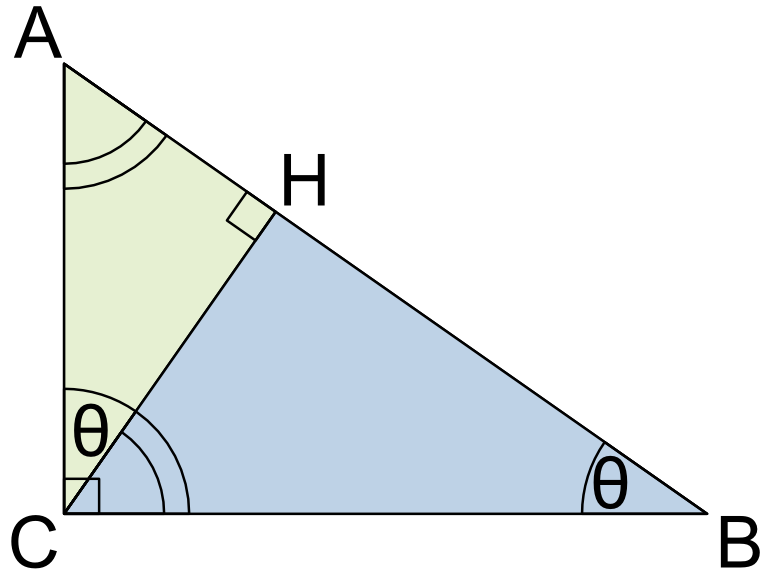
\includegraphics[width=0.3\textwidth]{figures/Pythagoras.png}
	\caption{Similar triangles used in the proof of the Pythagorean theorem.}
	\label{fig:Pythagoras}
\end{figure}

The new triangle $ACH$ is similar to triangle $ABC$, because they both have a right angle (by definition of the altitude), and they share the angle at $A$, meaning that the third angle will be the same in both triangles as well, marked as $\theta$ in Figure~\ref{fig:Pythagoras}. By a similar reasoning, the triangle $CBH$ is also similar to $ABC$. 

Similarity of the triangles leads to the equality of ratios of corresponding sides:
\begin{equation}
    \frac{BC}{AB}=\frac{BH}{BC} \text{ and } \frac{AC}{AB}=\frac{AH}{AC}.
\end{equation}
The first result equates $\cos \theta$ and the second result equates $\sin \theta$.

These ratios can be written as:
\begin{equation}
    {BC}^{2}={AB}\times {BH} \text{ and }{AC}^{2}={AB}\times {AH}.
\end{equation}
Summing these two equalities, we obtain:
\begin{equation}
    {BC}^{2}+{AC}^{2}={AB}\times {BH}+{AB}\times {AH}={AB}\times({AH}+{BH})={AB}^{2} ,
\end{equation}
which, tidying up, is the Pythagorean theorem:
\begin{equation}
    {BC}^{2}+{AC}^{2}={AB}^{2}.
\end{equation}
\end{proof}
%
\end{appendices}
%--------------------------------------------------------------------------------------------------
%
% BACK MATTER
%--------------------------------------------------------------------------------------------------
%
\backmatter
%
% References used in the thesis
\printreferences
%
% Author's bibliography
%--------------------------------------------------------------------------------------------------
% 
\chapter{Bibliography}
%--------------------------------------------------------------------------------------------------
% Enclose with refsection and use \nocite{*}, if you need to list publications not referenced in 
% the thesis:
\begin{refsection}
\nocite{*}

\section*{Publications Related to the Thesis}

All publications related to the thesis should be referenced in the text.

\defbibheading{subbibliography}{\subsection*{Journal Articles}}
\printbibliography[heading=subbibliography,env=nolabelbib,sorting=nty,keyword=myarticle]

\defbibheading{subbibliography}{\subsection*{Conference Paper}}
\printbibliography[heading=subbibliography,env=nolabelbib,sorting=nty,keyword=myconf]

\section*{Other Publications (optional)}

\dots

\end{refsection}
%
% Author's biography
%--------------------------------------------------------------------------------------------------
%
\chapter{Biography}
%--------------------------------------------------------------------------------------------------

Jan Rupnik was born in Ljubljana on 6.12.1982. 
 
Following graduation at the Faculty of Mathematics and Physics, University of Ljubljana, 
with a degree in applied mathematics (Diploma) in 2006, he was employed as a researcher 
at the Artificial Intelligence Laboratory, Jožef Stefan Institute. In 2007 he
enroled in the New Media and E-science doctoral study program at the Jožef Stefan 
International Postgraduate School in Ljubljana, Slovenia.

His research interests include Machine Learning, Data Mining, Data
Fusion, Cross-Lingual Text Mining, Predictive Analytics, Applications of Data Mining
in different domains. Most of his research work is connected to the development of
statistical methods that enable cross-modal data integration, with focus on
scalability. 

Jan Rupnik has been involved in a number of EU FP7 projects, including
SMART (Statistical Multilingual Analysis For Retrieval And Translation), XLIKE (Cross-
lingual Knowledge Extraction), EURIDICE (The Intelligent Cargo Concept in the
European Project) and SOPHOCLES (Self-Organised information PrOcessing,
CriticaLity and Emergence in multilevel Systems).
%
% Index (optional)
\printmyindex
%--------------------------------------------------------------------------------------------------
\end{document}
